\documentclass[JEP,XML,SOM,Unicode]{cedram}
\datereceived{2016-11-02}
\dateaccepted{2019-10-03}
\dateepreuves{2019-10-09}

\usepackage{mathrsfs}
\let\mathcal\mathscr

\newcommand{\Changel}{\mathcode`l="7160}
\newcommand{\Changelback}{\mathcode`l="716C}

\newcommand{\NoChangel}[1]{%
\expandafter\let\csname old\string#1\endcsname=#1
\let#1=\relax
\newcommand{#1}{\mathcode`l="716C\csname old\string#1\endcsname\mathcode`l="7160 }%
}

\NoChangel{\log}
\NoChangel{\ln}
\NoChangel{\lim}
\NoChangel{\limsup}
\NoChangel{\liminf}
\NoChangel{\varlimsup}
\NoChangel{\varliminf}
\NoChangel{\varinjlim}
\NoChangel{\varprojlim}

\AtBeginDocument{%
\renewcommand{\theenumi}{\roman{enumi}}%
}

\let\oldbigsqcup\bigsqcup
\renewcommand{\bigsqcup}{\mathop{\textstyle\oldbigsqcup}\displaylimits}
\def\mto{\mathchoice{\longmapsto}{\mapsto}{\mapsto}{\mapsto}}
\def\hto{\mathrel{\lhook\joinrel\to}}
\def\To#1{\mathchoice{\xrightarrow{\textstyle\kern4pt#1\kern3pt}}{\stackrel{#1}{\longrightarrow}}{}{}}
\def\From#1{\mathchoice{\xleftarrow{\textstyle~#1~}}{\stackrel{#1}{\longleftarrow}}{}{}}
\newenvironment{smallpmatrix}{\big(\begin{smallmatrix}}{\end{smallmatrix}\big)}

\newcommand{\Aff}{\mathit{Aff}}
\newcommand{\Ana}{\mathit{Ana}}
\newcommand{\Han}{\mathit{Han}}
\newcommand{\Man}{\mathit{Man}}
\newcommand{\adj}{\mathrm{adj}}
\newcommand{\sat}{\mathrm{sat}}
\newcommand{\so}{\mathrm{so}}
\newcommand{\GL}{\mathrm{GL}}
\newcommand{\PSL}{\mathrm{PSL}}
\newcommand{\SL}{\mathrm{SL}}
\DeclareMathOperator{\Aut}{Aut}
\DeclareMathOperator{\Diff}{Diff}
\DeclareMathOperator{\Hol}{Hol}\NoChangel{\Hol}
\DeclareMathOperator{\Hom}{Hom}
\DeclareMathOperator{\Id}{Id}
\DeclareMathOperator{\Imm}{Im}\let\Im\Imm
\DeclareMathOperator{\Ree}{Re}\let\Re\Ree
\DeclareMathOperator{\Tr}{Tr}

\usepackage{graphicx}
\usepackage{tikz-cd}
\tikzcdset{every label/.append style = {font = \normalsize}}

\theoremstyle{plain}
\newtheorem{theorem}{Theorem}[section]
\newtheorem{corollary}[theorem]{Corollary}
\newtheorem{proposition}[theorem]{Proposition}
\newtheorem{lemma}[theorem]{Lemma}

\theoremstyle{definition}
\newtheorem{definition}[theorem]{Definition}
\newtheorem{example}[theorem]{Example}
\theoremstyle{remark}
\newtheorem{remark}[theorem]{Remark}
\newtheorem{hypothesis}[theorem]{Hypothesis}
\newtheorem{remarks}[theorem]{Remarks}
\newtheorem{question}[theorem]{Question}
\newtheorem{problem}[theorem]{Problem}
\newtheorem{convention}[theorem]{Convention}

\numberwithin{equation}{section}

\newcommand{\CC}{{\mathbb{C}}}
\newcommand{\Azero}{\Aut^0(X_0)}
\newcommand{\Aun}{\Aut^1(X_0)}
\newcommand{\T}{\mathcal T(X)}
\newcommand{\D}{\Diff^0(X)}
\newcommand{\DlKz}{\Diff^0_l(X,\mathcal K_0)}
\newcommand{\DK}{\Diff^0(X,\bigsqcup_{\alpha\in A}\mathcal K_\alpha)}
\newcommand{\DKp}{\Diff^+(X,\bigsqcup_{\alpha\in A}\mathcal K_\alpha)}
\newcommand{\cI}{\mathcal{I}}

\let\uniondisjointe\bigsqcup

\begin{document}
\frontmatter

\title{The Teichmüller and Riemann moduli stacks}

\author[\initial{L.} \lastname{Meersseman}]{\firstname{Laurent} \lastname{Meersseman}}
\address{LAREMA, Université d'Angers\\
F-49045 Angers Cedex, France}
\email{laurent.meersseman@univ-angers.fr}
\urladdr{https://math.univ-angers.fr/membre/meersseman-laurent/}

\thanks{This is part of project Marie Curie 271141 DEFFOL}

\dedicatory{To Alberto Verjovsky on his 70th birthday.\vspace*{\baselineskip}}

\subjclass{32G05, 58H05, 14D23}

\keywords{Teichmüller space, deformations of complex structures, analytic groupoids, stacks and moduli problems}

\begin{abstract}
The aim of this paper is to study the structure of the Teichmüller and \hbox{Riemann} moduli spaces, viewed as stacks over the category of complex analytic spaces, for higher-dimensional manifolds. We show that both stacks are analytic in the sense that they are isomorphic to the stackification of a smooth analytic groupoid. We then show how to construct explicitly such an atlas as a sort of generalized holonomy groupoid. This is achieved under the sole condition that the dimension of the automorphism group of each structure is bounded by a fixed integer. All this can be seen as an answer to Question 1.8 of \cite{VerbitskySurvey}.
\end{abstract}

\alttitle{Les champs de modules de Teichmüller et de Riemann}

\altkeywords{Espace de Teichmüller, déformations de structures complexes, groupoïdes analytiques, champs et problèmes de modules}

\begin{altabstract}
Le but de cet article est d'étudier la structure des espaces de modules de Teichmüller et de Riemann de variétés de dimension plus grande que $1$, considérés comme des champs sur la catégorie des espaces analytiques complexes. Nous montrons que ces deux champs sont analytiques, c'est-à-dire isomorphes à la champification d'un groupoïde analytique lisse. Nous donnons ensuite une construction explicite d'atlas comme groupoïde d'holonomie généralisé. Ces résultats sont valables dès que la dimension du groupe d'automorphismes de chaque structure est bornée par un entier fixé. On peut voir ce travail comme une réponse à la question 1.8 de \cite{VerbitskySurvey}.
\end{altabstract}

\maketitle
\tableofcontents
\mainmatter

\section{Introduction}
\label{intro}
Let $X$ be a smooth oriented compact surface. The \emph{Riemann moduli space} $\mathcal M^s(X)$ is defined as the set of Riemann surfaces $C^\infty$-diffeomorphic to $X$ up to biholomorphism. Thus each point of $\mathcal M^s(X)$ encodes a complex structure on $X$ and two different points correspond to two non-biholomorphic complex structures.

In the same way, the \emph{Teichmüller space} $\mathcal T^s(X)$ is roughly defined as the set of \hbox{Riemann} surfaces diffeomorphic to $X$ up to biholomorphism $C^\infty$-isotopic to the identity (see Section \ref{TRspaces}).

The theory of Teichmüller spaces is a cornerstone in complex variables and Riemann surfaces. Originated by Riemann himself and followed by the fundamental works of Teichmüller, Ahlfors and Bers, it has moreover implications in many branches of mathematics as algebraic geometry, hyperbolic geometry, complex dynamics, discrete groups, ...

Perhaps the most basic property of $\mathcal T^s(X)$ is that
it has a natural structure of a complex manifold.

Moreover, the mapping class group of $X$ acts on $\mathcal T^s(X)$ and the resulting quotient is a complex orbifold. This refined quotient coincides with $\mathcal M^s(X)$, which thus acquires a natural structure of a complex orbifold.

Let now $X$ be a smooth oriented compact manifold of even dimension $2n$ strictly greater than $2$. The Teichmüller and Riemann moduli spaces can still be defined in the same way, replacing above ``Riemann surfaces'' with ``complex manifolds''.

Although the literature about these higher dimensional Teichmüller and Riemann moduli spaces is much less developed than that about surfaces, it has grown significantly in the last years and these spaces play an increasing role in complex geometry. Catanese's guide to deformations and moduli \cite{Catsurvey} as well as \cite{Catsurvey2} gives some general local properties of $\mathcal T^s(X)$ and contains many results on the Teichmüller space of minimal surfaces of general type. And in the special case of hyperkähler manifolds, the Teichmüller space is used by Verbitsky in a prominent way in his proof of a global Torelli theorem \cite{Verbitsky} and also to showing some important results on these manifolds \cite{VerbitskyErgodic}.

However, the main difference with the case of surfaces is that $\mathcal T^s(X)$ and $\mathcal M^s(X)$ are \emph{just topological spaces} and do not have any good geometric structure. Only for special classes such as the class of hyperkähler manifolds, an analytic structure is known on $\mathcal T^s(X)$, but even in this case, it is not Hausdorff at all points. Perhaps the most dramatic example is given by $X$ being $\mathbb S^2\times\mathbb S^2$. Then $\mathcal M^s(X)$, \emph{as a set}, can be identified with $\mathbb N$, a point $a\in\mathbb N$ corresponding to the Hirzebruch surface $\mathbb F_{2a}$ (and each connected component of $\mathcal T^s(X)$ can be identified with $\mathbb Z$, $a$ and $-a$ encoding the same surface, see Examples \ref{Hirzebruch} and \ref{Hirzebruchbis}). But, \emph{as a topological space}, it is endowed with a non-Hausdorff topology. No two points are separated, as a consequence of the fact that $\mathbb F_{2a}$ can be deformed onto any $\mathbb F_{2b}$ with $b<a$ by an arbitrary small deformation. Equivalently, this comes from the fact that the dimension of the automorphism group of Hirzebruch surfaces jumps.

Indeed, in presence of this jumping phenomenon, $\mathcal T^s(X)$ and $\mathcal M^s(X)$ are not even locally Hausdorff hence not locally isomorphic to an analytic space (\cf Example \ref{Hopfbis}). This explains why the classical approach developed in the fundamental works of Kodaira-Spencer and Kuranishi is based on the following principles.
\begin{enumerate}
\item
In higher dimension the global point of view must be abandoned for the local point of view;
\item
and the Teichmüller space replaced with the Kuranishi space which must be thought of as the best possible approximation in the analytic category for a local moduli space of complex structures.
\end{enumerate}

We emphasize that the Kuranishi space is in general not locally homeomorphic to the Teichmüller space (\cf Remark \ref{localmodeldifference}), hence Kodaira-Spencer's reduction is far from being simply a reduction to the local case.

Nevertheless, putting on $\mathcal T^s(X)$ and $\mathcal M^s(X)$ a global analytic structure in some sense is the only way to go beyond the classical local deformation theory. As we cannot expect a structure of analytic space, even a non-Hausdorff one, \emph{we have to view these quotient spaces as stacks}. The aim of this paper is to develop this point of view. We~turn the topological spaces $\mathcal T^s(X)$ and $\mathcal M^s(X)$ into stacks $\T$ and $\mathcal M(X)$ over the category of finite-dimensional analytic spaces. The question now becomes to showing that, \emph{as stacks, $\T$ and $\mathcal M(X)$ are analytic}. This can also be seen as an answer to Question 1.8 of \cite{VerbitskySurvey}. Since we work with arbitrary complex structures and not only with projective ones, we have to work with analytic stacks and not algebraic ones.

For surfaces of fixed genus $g>1$, the classical setting coincide with the stack setting. Both stacks $\T$ and $\mathcal M(X)$ are analytic and can be fully recovered from $\mathcal T^s(X)$ and $\mathcal M^s(X)$. In particular, the complex structure on $\mathcal T^s(X)$, respectively the complex orbifold structure on $\mathcal M^s(X)$ are equivalent to the analytic structures on the corresponding stack. The case of genus $1$ is somewhat more complicated because of the translations.\footnote{To avoid this problem, it is customary to use marked complex tori, that is, elliptic curves.} Here, the stack structure contains strictly more information than the classical spaces $\mathcal T^s(X)=\mathbb H$ and $\mathcal M^s(X)=\mathbb H/\PSL_2(\mathbb Z)$ since it also encodes the translation group of each complex torus, but once again both stacks are analytic and their analytic structure comes from the complex structure on the corresponding spaces.

The main results of this paper show that, in any dimension, both the Teichmüller and the Riemann moduli stacks are analytic stacks. The only condition needed for this result to hold is that the dimension of the automorphism group of all structures of $\mathcal T(X)$ (or $\mathcal M(X)$) is bounded by a fixed integer.\footnote{which is always the case for surfaces.} This is nevertheless a mild restriction since we may easily decompose them into strata where this dimension is bounded. We emphasize that $X$ can be any compact manifold and that we consider all complex structures and not only projective or Kähler ones.

It is also worth highlighting that, rather than considering all the complex structures on $X$, we may restrict ourselves to an open subset of it. Since Kählerianity is an open property by a famous theorem of Kodaira-Spencer \cite[Th.\,4.6]{MK}, our results also apply to the set of Kähler structures on $X$ modulo biholomorphism or modulo biholomorphism $C^\infty$-isotopic to the identity. Moreover, since the full set of complex structures is known for very few $X$, in many examples, it is interesting to restrict to an open subset.

We postpone the precise statements of the main theorems \ref{maintheorem} and \ref{mainR} as well as the strategy of proof to Section \ref{notations} after defining precisely the involved notions. Let us just say that we will follow the same strategy that can be used for Riemann surfaces. Firstly, we define $\mathcal T(X)$ and $\mathcal M(X)$ as stacks of families of complex manifolds diffeomorphic to $X$ in Section \ref{stacks}. This is the easy part. Secondly, we build an atlas with good analytic properties to show they are analytic in the sense of Section \ref{groupoidatlas}. This is the difficult part which takes the rest of the paper.

We hope that this paper will serve as a source of motivation for studying global moduli problems in complex analytic geometry and their interplay with analytic stacks. From the one hand, every abstract result on these stacks might apply to moduli problems and increase our knowledge of complex manifolds. From the other hand, examples of Teichmüller stacks are an unending source of examples of analytic stacks, showing all the complexity and richness of their structure, far from finite dimensional group actions and leaf spaces.

\subsubsection*{Acknowledgements}
I enjoyed the warm atmosphere of the CRM at Bellaterra during the preparation of this work. I would like to thank Ernesto Lupercio for explaining me the basics of groupoids and their interest in moduli theory; Alain Genestier for suggesting the construction of Section \ref{Teichmueller} and for stimulating discussions about stacks; Allen Hatcher and Daniel Ruberman for answering some questions about the mapping class group of $4$-manifolds; Fabrizio Catanese for discussions about the rigidified hypothesis of Section \ref{rigidified}; Serge Cantat for pointing out a result of Liebermann on automorphisms of Kähler manifolds; and Etienne Mann for clarifying some aspects of algebraic stacks. Finally many thanks to the referees whose accurate comments gave rise to a greatly improved version of the paper.

\section{Definitions of the Teichmüller and Riemann stacks and statement of the main results}
\label{notations}

\subsection{The Teichmüller and Riemann spaces}
\label{TRspaces}
Let us first review the precise definitions of Teichmüller and Riemann moduli spaces as well as of their topology. Let~$X$ be a smooth (\ie $C^\infty$) oriented compact connected manifold of even dimension. Assume that it admits complex structures. As done in the introduction, we can formally define its moduli space as the set of complex manifolds diffeomorphic to $X$ up to biholomorphisms. In short,
\begin{equation}
\label{M}
\mathcal M^s(X)=\{Y\text{ complex manifold}\mid Y\simeq_{\so} X\}/\sim,
\end{equation}
where $X\simeq_{\so}Y$ means that there exists a $C^\infty$-diffeomorphism from $Y$ to $X$ preserving the orientations and where $Y\sim Y'$ if they are biholomorphic.

Thanks to the Newlander-Nirenberg theorem \cite{NN}, a structure of a complex manifold on $X$ is equivalent to an integrable complex operator $J$ on $X$, that is, a $C^\infty$ bundle operator $J$ on the tangent bundle $TX$ such that
\begin{equation}
\label{ico}
J^2=- \Id\quad\text{ and }\quad [T^{0,1},T^{0,1}]\subset T^{0,1}
\end{equation}
for
\begin{equation}
\label{T01}
T^{0,1}=\{v+iJv\mid v\in TX\otimes\CC\}
\end{equation}
the subbundle of the complexified tangent bundle $TX\otimes\CC$ formed by the eigenvectors of $J$ with eigenvalue $-i$. Here of course, $J$ has been linearly extended to the complexified tangent bundle. We may thus rewrite \eqref{M} as
\begin{equation}
\label{M2}
\mathcal M^s(X)=\{J\text{ o.p. integrable complex operator on } X\}/\sim,
\end{equation}
where o.p. means orientation preserving, \ie the orientation induced on $X$ by $J$ coincides with that of $X$.

Now, it is easy to check that $(X,J)$ and $(X,J')$ are biholomorphic if and only if there exists a diffeomorphism $f$ of $X$ whose differential $df$ satisfies
\begin{equation}
\label{Jf}
J'=(df)^{-1}\circ J\circ df.
\end{equation}
In other words, setting
\begin{equation}
\label{I}
\cI=\{J\ :\ TX\longrightarrow TX\mid J^2\equiv -\Id,\ J\text{ o.p.},\ \ [T^{1,0}, T^{1,0}]\subset T^{1,0}\}
\end{equation}
and denoting $J\cdot f$ the right hand side of \eqref{Jf}, we see that \eqref{Jf} defines a right action of the diffeomorphism group $\Diff(X)$ onto $\cI$. Since our operators are o.p., this is even in fact an action of $\Diff^+(X)$, the group of diffeomorphisms of $X$ that preserve the orientation.

So we end with
\begin{equation}
\label{Riem}
\mathcal M^s(X):=\cI\big /\Diff^+(X)
\end{equation}
and we are in position to define the \emph{Teichmüller space} of $X$ as
\begin{equation}
\label{Teich}
\mathcal T^s(X):=\cI\big /\Diff^0(X),
\end{equation}
where $\Diff^0(X)$ is the group of diffeomorphisms $C^\infty$-isotopic to the identity, that is, the connected component of the identity in $\Diff^+(X)$.

Alternatively, if we define the mapping class group as the group
\begin{equation}
\label{mcgroup}
\mathcal M\mathcal C(X):=\Diff^+(X)\big /\Diff^0(X)
\end{equation}
we have
\begin{equation}
\label{TeichRiem}
\mathcal M^s(X)=\mathcal T^s(X)\big /\mathcal M\mathcal C(X).
\end{equation}
It is important to notice that \eqref{Riem} and \eqref{Teich} define \emph{topological spaces} and not only sets as \eqref{M}. Indeed, we endow $\cI$ and $\Diff(X)$ with the topology of $C^\infty$ convergence: a~sequence of operators/functions tends to zero if it converges to zero for every $C^k$\nobreakdash-norm with $k\geq 0$ on every compact set, \cf \cite{Hamilton}. And we endow \eqref{Riem}, \eqref{Teich} and \eqref{mcgroup} with the quotient topology. Observe that $\mathcal M\mathcal C(X)$ is a discrete topological group, since every diffeomorphism close enough to the identity is isotopic to the identity.\footnote{This classical fact can be proved using the Fréchet chart introduced in \eqref{Frechetchart}.}

Moreover, let $\mathcal E$ denote the set of $C^\infty$ o.p. almost complex operators, that is
\begin{equation}
\label{E}
\mathcal E=\{J\ :\ TX\longrightarrow TX\mid J^2\equiv -\Id,\ J\text{ o.p.}\}.
\end{equation}
It is easy to prove that the action of $\Diff^+(X)$ on $\mathcal E$ is continuous and preserves $\cI$. We will see in Section \ref{FrHilb} that each diffeomorphism acts as a complex analytic isomorphism of $\mathcal E$, once $\mathcal E$ and $\cI$ are endowed with suitable complex Hilbert structures.

Some notations to conclude this section. We denote by $\mathcal E_0$, respectively $\cI_0$, a connected component of $\mathcal E$, respectively $\cI$. Points of $\mathcal E$ will be denoted generically by $J$. For a topological space $T$, we denote by $\pi_0(T)$ the set of connected components of $T$. The previous topology being countable, $\pi_0(\mathcal E)$ is a countable set.
\begin{remark}
\label{oriented}
In the first version of this paper, we took for $X$ an unoriented smooth compact manifold and considered $\cI$ as the set of all integrable complex operators, regardless of orientation. Then $\mathcal T^s(X)$ was defined as in \eqref{Teich}, and in \eqref{Riem}, the full diffeomorphism group $\Diff(X)$ replaced the oriented diffeomorphism group. This does not change substantially these two sets, and our results apply to this setting. In fact, the main drawback of forgetting the orientation is that the notion of Teichmüller space does not coincide with the classical one for surfaces. Especially, the unoriented Teichmüller space of a compact surface has two connected components, corresponding to the two possible orientations.

More generally, if $X$ admits a diffeomorphism reversing orientation, then the unoriented Teichmüller space has twice more connected components as the classical one. However, the two Riemann spaces coincide. Finally, if $X$ does not admit any orientation reversing diffeomorphism, then the unoriented Teichmüller and Riemann spaces are the disjoint union of the classical ones for both orientations. Notice that, in this last case, changing the orientation may completely change the Teichmüller and \hbox{Riemann} spaces. It is even possible that they become empty. For example, let $X$ be the oriented $C^\infty$ manifold underlying $\mathbb P^2$ and let $\overline{X}$ be equal to $X$ with the orientation reversed (which is sometimes denoted by $\overline{\mathbb P^2}$, although it may be very confusing since it is not a complex manifold). We claim that $\overline{X}$ does not admit any almost complex structure compatible with its orientation. Assume the contrary and let $J$ be a compatible almost complex structure on $\overline{X}$. Then Wu's formula applies and yields
\begin{equation*}
\tau(\overline{X})=\dfrac{1}{3}(c_1^2(\overline{X},J)-2c_2(\overline{X},J)).
\end{equation*}
Now the Chern numbers $c_1^2$ and $c_2$ do not depend on the almost-complex structure. They are indeed (unoriented) topological invariants so are equal to those of $\mathbb P^2$. Hence $c_1^2=9$ and $c_2=3$. Then, $X$ has signature $1$, so $\overline{X}$ has signature $-1$. These numbers do not satisfy the above formula and the claim is proved. As a consequence, the Teichmüller and Riemann spaces of $\overline{X}$ are empty. Note that the Riemann space of~$X$ is reduced to a point by Yau's theorem; and since every automorphism of $\mathbb P^2$ is isotopic to the identity, so is the Teichmüller space of $\mathbb P^2$.
\end{remark}

\subsection{Stacks}
\label{stacksgroupoids}
Before getting into the definition of the Teichmüller and Riemann moduli stacks, let us define precisely the notion of stacks we will use.

First, a warning. We insist on the fact that we work exclusively in the $\CC$-analytic context, since we deal with arbitrary compact complex
manifolds. This forces us to adapt and sometimes to transform the definitions of stacks coming from algebraic geometry. Also, since the literature on stacks over the category of analytic spaces is very scarce, we shall keep the required facts from stack theory to a minimum and give complete proofs even of some routine facts (for example in Proposition \ref{Theyarestacks}).

Moreover, our construction of atlas (see Section \ref{groupoidatlas}) is inspired from the construction of the étale holonomy groupoid of a foliation. So for the atlas point of view, we stick to the literature in foliation theory and Lie groupoids, especially \cite{Moerdijk}. The conventions are somewhat different from those of algebraic geometry and we have to adapt ourselves to these differences. Especially, we will not make use of the notion of representability of the diagonal, see Section \ref{groupoidatlas}.

We will only consider stacks over the analytic site defined as follows. Let $(\Ana)$ \hbox{denote} the category of finite-dimensional $\CC$-analytic spaces. We include analytic spaces that are everywhere non-reduced in $(\Ana)$. We consider it as a site for the \hbox{Euclidean} topology: our families of coverings are just standard topological open coverings. We~emphasize that we will not use other coverings as étale or analytic ones.

In this paper, a \emph{stack} $p:\mathcal S\to (\Ana)$ is a stack in groupoids over the site $(\Ana)$ in the sense of \cite[Def.\,8.5.1]{Stacksproject}.
In brief, a functor $p:\mathcal S\to (\Ana)$ is a stack if
\begin{enumerate}
\item
$p:\mathcal S\to(\Ana)$ is a category fibered in groupoids, \ie the fibers of $p$ are groupoids, pull-backs exist and are unique up to unique isomorphisms,
\item
isomorphisms form a sheaf, \ie one can glue a compatible collection of isomorphisms defined over an open covering of an analytic space $S$ into a single isomorphism over $S\to S$,
\item
every descent data is effective, \ie one can glue objects defined on an open covering of an analytic space $S$ into a single object over $S$ by means of a cocycle of morphisms.
\end{enumerate}

\subsection{The Teichmüller and Riemann moduli stacks}
\label{stacks}
We are now in position to define the Teichmüller and Riemann moduli \emph{stacks}, which are the main protagonists of this paper. In fact, we will define such stacks over any open set of $\cI$.

Let $V$ be an open set of $\cI$. Define the following category $\mathcal M(X,V)$ over $(\Ana)$. \emph{Objects} are $(X, V)$-families
\begin{equation}
\label{XVfamily}
\pi\ :\ \mathcal X\longrightarrow B,
\end{equation}
that is:
\begin{enumerate}
\item
$B\in (\Ana)$ and $\mathcal X\in(\Ana)$,

\item
$\pi$ is a smooth and proper morphism with fibers all diffeomorphic to $X$,

\item
each fiber $X_b:=\pi^{-1}(b)$ can be encoded as $(X, J)$ with $J\in V$.
\end{enumerate}
Recall that smooth means flat with smooth fibers. Hence, the fibers are complex manifolds, say of dimension $n$, and for any $x\in\mathcal X$, there exist a neighborhood $U$, a neighborhood $W$ of $0$ in $\CC^n$ and an isomorphism $\phi$ of $U$ onto the product $\pi(U)\times W$ such that the following diagram commutes
\begin{equation}
\label{flatness}
\begin{tikzcd}[column sep=tiny, row sep=normal]
U \arrow[rrr,"\phi"] \arrow[rrd, end anchor = north west,"\pi"'] &&&\pi(U)\times W\arrow[dl, start anchor = south, end anchor = north east,"\text{1st proj.}"]\\
&&\pi (U)&
\end{tikzcd}
\end{equation}
In other words, a $(X, V)$-family is nothing else than an analytic deformation of complex structures of $X$ such that the structure of each fiber is isomorphic to a point of $V\subset \cI$. Of course, if $V^{\sat}$ denotes the image of $V$ through the action of $\Diff^+(X)$, then $\mathcal M(X,V)$ and $\mathcal M(X,V^{\sat})$ are equal. However, it is interesting to have this flexibility, for example we will often take for $V$ a connected component of $\cI$, even if it is not saturated.

\emph{Morphisms} are Cartesian diagrams
\begin{equation}
\label{XVmorphisms}
\begin{tikzcd}
\mathcal X\arrow[r,"F"]\arrow[d,swap,"\pi"]&\mathcal X'\arrow[d,"\pi'"]\\
B\arrow[r,"f"]&B'
\end{tikzcd}
\end{equation}
between $(X,V)$-families. Observe that the pull-back of a $(X,V)$-family is a $(X,V)$-family.

We equip $\mathcal M(X,V)$ with a morphism $p:\mathcal M(X,V)\to (\Ana)$ which sends a $(X,V)$-family $\mathcal X\to B$ onto its base $B$, and a morphism \eqref{XVmorphisms} onto the base morphism $B\to B'$.

We now pass to the construction of $\mathcal T(X, V)$, which is more delicate. Consider $\mathcal X$ and $B$ as real analytic spaces, and $\pi$ as a real analytic flat morphism, hence consider real analytic trivializations \eqref{flatness}. Then, using the fact that the first cohomology group of every fiber with values in the sheaf of germs of real analytic vector fields is zero, we may apply the proof by power series methods of \cite[Th.\,3.2]{MK} to conclude that the restriction $\mathcal X_{\vert B_\alpha}$ of $\mathcal X$ over some sufficiently small open set $B_\alpha\subset B$ is locally isomorphic to a product, that is, that we have bundle real analytic trivializations\footnote{In the diagram \eqref{flatnessbis}, we endow the compact $C^\infty$-manifold $X$ with its real analytic structure.}
\begin{equation}
\label{flatnessbis}
\begin{tikzcd}[column sep=tiny, row sep=normal]
\mathcal X_{\vert B_\alpha}\arrow[rrr,"\simeq"] \arrow[rrd, end anchor = north west,"\pi"'] &&&B_\alpha\times X\arrow[dl, start anchor = south, end anchor = north east,"\text{1st proj.}"]\\
&&B_\alpha&
\end{tikzcd}
\end{equation}
In particular, such a trivialization induces real analytic isomorphisms between the complex manifold $\pi^{-1}(b)$ and the real analytic $X\times\{b\}$ for every $b\in B_\alpha$ and we may thus transfer the complex structure along the fibers of $\pi$ to a real analytic family $\mathcal J_\alpha=(J_b)_{b\in B_\alpha}$ of complex operators of $X$. Thus, the real analytic fiber preserving isomorphism
\begin{equation}
\label{trivialization}
\mathcal X_{\vert B_\alpha}\simeq (X\times B_\alpha, \mathcal J_\alpha)
\end{equation}
becomes holomorphic on the fibers, see \cite[Th.\,4.5]{Cat}, \cite[\S 2.3]{circle} and \cite[Prop.\,1]{DouadyBourbaki}. Over an intersection $B_\alpha\cap B_\beta$, two trivializations \eqref{trivialization} are glued using a family $(\phi_t)_{t\in B_\alpha\cap B_\beta}$ of diffeomorphisms of $X$ whose differential commute with $\mathcal J_\alpha$ and $\mathcal J_\beta$. As a consequence, $\mathcal X$ is diffeomorphically a bundle over $B$ with fiber $X$ and structural group $\Diff^+(X)$. In particular, once such an identification with a bundle is fixed, it makes sense to speak of the structural group of $\mathcal X$, and to make a reduction of the structural group to some subgroup $H$ of $\Diff^+(X)$. And it makes also sense to speak of $H$-isomorphism of the family $\mathcal X$, that is, isomorphism of $\mathcal X$ such that, in each fiber, the induced diffeomorphism of $X$ is in $H$.

We define $\mathcal T(X,V)$ as the category whose objects are $(X,V)$-families with a marking\vspace*{-3pt}
\begin{equation}
\label{XVfamilymarked}
\begin{tikzcd}[column sep=tiny, row sep=normal]
\mathcal X\arrow[rrr,"\simeq"] \arrow[rrd, end anchor = north west,"\pi"'] &&&E\arrow[dl, end anchor = north east]\\
&&B&
\end{tikzcd}
\end{equation}
with $E\to B$ a bundle with fiber $X$ and structural group reduced to $\Diff^0(X)$ and whose morphisms are Cartesian diagrams \eqref{XVmorphisms} such that the canonical isomorphism between $\mathcal X$ and $f^*\mathcal X'$ induces a $\Diff^0(X)$-isomorphism of the markings.

Alternatively, one may use $\D$-framings, that is, $C^\infty$-isotopy classes of maps%
\begin{equation}
\begin{tikzcd}
X \arrow[r,"\simeq", "i"']&\pi^{-1}(b)\ \arrow[d,swap,"\pi"]\arrow[r,hook]&\mathcal X\arrow[d,"\pi"]\\
&b\arrow[r,hook] &B
\end{tikzcd}
\end{equation}
Here, $b$ is any point of $B$ and isotopies are $C^\infty$-maps $I$ from $X\times [0,1]$ to $\mathcal X$ such that $\pi\circ I(X\times\{t\})$ is a point for all $t\in [0,1]$. In particular, we may replace $b$ by any other point using an isotopy. Set $I_t:=I(-,t)$. Since $\mathcal X\to B$ is diffeomorphic to a $\D$-bundle, then, given an isotopy $I$ with $\pi\circ I(X\times\{0\})=\pi\circ I(X\times\{1\})$, the diffeomorphism $I_1^{-1}\circ I_0$ of $X$ belongs to $\D$. In other words, the framing induces in that case a coherent identification of the fibers with $X$ up to an element of $\D$.

This forms a category over $(\Ana)$ and a subcategory of $\mathcal M(X,V)$. In general, it contains strictly less objects, since some $(X,V)$-families do not admit $C^\infty$-markings. It comes equipped with the same morphism $p : \mathcal T(X,V)\to (\Ana)$.

\begin{proposition}
\label{Theyarestacks}
Let $V$ be an open subset of $\cI$. Then both $p: \mathcal M(X,V)\to (\Ana)$ and $p: \mathcal T(X,V)\to (\Ana)$ are stacks.
\end{proposition}

\begin{proof}
It is straightforward but we sketch it for sake of completeness. First, the natural morphism $p:\mathcal M(X,V)\to(\Ana)$ is obviously a category fibered in groupoids. The fiber over $S\in(\Ana)$ is the groupoid formed by $(X,V)$-families over $S$ as \hbox{objects} and isomorphisms of families as morphisms. Then, given two $(X,V)$-families \hbox{$\pi : \mathcal X\to S$} and $\pi' : \mathcal X'\to S$ and an open covering $(S_\alpha)$ of $S$, any collection of isomorphisms $f_\alpha$ from the restriction of $\mathcal X$ to $\pi^{-1}(S_\alpha)$ onto the restriction of $\mathcal X'$ to $(\pi')^{-1}(S_\alpha)$ such that $f_\alpha$ and $f_\beta$ are equal on the intersections $\pi^{-1}(S_\alpha\cap S_\beta)$ obviously glue to give an isomorphism of families between $\mathcal X$ and $\mathcal X'$. So isomorphisms form a sheaf. Finally, starting from a collection $\pi_\alpha :\mathcal X_\alpha\to S_\alpha$ of $(X,V)$-families and from a cocycle $f_{\alpha\beta}$ of isomorphisms of families between $\pi^{-1}_\alpha (S_\alpha\cap S_\beta)$ and $\pi^{-1}_\beta (S_\alpha\cap S_\beta)$, then
\[
\mathcal X:=\uniondisjointe \mathcal X_\alpha/\equiv,
\]
where $\equiv$ is the equivalence relation given by the cocycle $(f_{\alpha\beta})$, is a $(X,V)$-family over~$S$. Every descent data is effective. The proof for $p:\mathcal T(X,V)\to (\Ana)$ is similar.
\end{proof}
\begin{convention}
Since we exclusively work over the site $(\Ana)$, we will simply denote by $\mathcal M(X,V)$, \resp $\mathcal T(X,V)$ the stack $p:\mathcal M(X,V)\to(\Ana)$, resp.\ \hbox{$p:\mathcal T(X,V)\to (\Ana)$}.
\end{convention}
Given $J\in\cI$, recall that $(X,J)$ is a complex manifold diffeomorphic to $X$ by use of the Newlander-Nirenberg theorem. Observe the following result.

\begin{lemma}
\label{stackspoints}
The points of $\mathcal M(X,V)$ are classes of biholomorphisms of complex manifolds $(X,J)$ with $J\in V$.

And the points of $\mathcal T(X,V)$ are classes of biholomorphisms $C^\infty$ isotopic to the identity of complex manifolds $(X,J)$ with $J\in V$.
\end{lemma}

\begin{proof}
This just means that, given $J\in V$, the fiber of $\mathcal M(X,V)\to(\Ana)$ over the point $J$ is the groupoid with $(X,J)$ as single object and with biholomorphisms of $(X,J)$ as isomorphisms; and the fiber of $\mathcal T(X,V)\to(\Ana)$ over the point $J$ is the groupoid with $(X,J)$ as single object and with biholomorphisms of $(X,J)$ smoothly isotopic to the identity as isomorphisms. And this is immediate from the definitions of these two stacks.
\end{proof}
We may thus define the following stacks.
\begin{definition}
\label{RMS}
We call \emph{Riemann moduli stack} the stack $\mathcal M(X,\cI)$. The stack $\mathcal M(X, V)$ is the Riemann moduli stack for complex structures belonging to $V$.
\end{definition}

By abuse of notation, we simply denote by $\mathcal M(X)$ the Riemann moduli stack. Because of Lemma \ref{stackspoints}, this must be thought of as the stack version of \eqref{M} and \eqref{Riem}, whereas $\mathcal M(X, V)$ is the stack version of $V/\Diff^+(X)$. In the same way,

\begin{definition}
\label{TMS}
We call \emph{Teichmüller stack} the stack $\mathcal T(X,\cI)$. The stack $\mathcal T(X, V)$ is the Teichmüller stack for complex structures belonging to $V$.
\end{definition}

By abuse of notation, we simply denote by $\mathcal T(X)$ the Teichmüller stack. Because of Lemma \ref{stackspoints}, this must be thought of as the stack version of \eqref{Teich}, whereas $\mathcal T(X, V)$ is the stack version of $V/\Diff^0(X)$.

\subsection{Groupoids and atlases}
\label{groupoidatlas}
We want to prove that $\T$ and $\mathcal M(X)$ are \emph{analytic stacks} and not only stacks over the analytic site. We observe that there is no standard definition of analytic stacks, so we have to forge this notion. Of course, it should be closely related to that of algebraic stacks.

So, let us make a detour to algebraic geometry to see how things happen there and how we can adapt them to our analytic world. Assume that we are given a stack $\mathcal S$ in groupoids as before but over an algebraic site, for example the site $(\Aff)$ of affine schemes over $\CC$ with étale coverings, and say we want to
prove that $\mathcal S\to (\Aff)$ is an \emph{algebraic stack}. Lemma \ref{stackspoints} shows that the isotropy group of a point of either $\T$ or $\mathcal M(X)$ is a complex Lie group and may thus be far from being finite, so wee need to look at Artin stacks and not at Deligne-Mumford stacks.

Standard definitions of algebraic stacks (Artin stacks), see for example \cite[Def.\,86.12.1]{Stacksproject} or \cite[Def.\,15.9]{BCEFFGK}, ask for representability of the diagonal by algebraic spaces and existence of a surjective, smooth morphism $U\to\mathcal S$ from a scheme $U$ onto the stack,\footnote{Some additional technical properties of the diagonal as separability or quasi-compactness may be required, but this is not important in this discussion.} called atlas of the stack. From the atlas, one constructs the groupoid $U\times_{\mathcal S}U\rightrightarrows U$ with source and target maps $s$ and $t$ fitting in the following Cartesian diagram
\begin{equation}
\label{symgroup}
\begin{tikzcd}
U\times_{\mathcal S}U \arrow[d,"t"']\arrow[r,"s"]&U\arrow[d]\\
U \arrow[r]&\mathcal X
\end{tikzcd}
\end{equation}
Then, the condition on the diagonal ensures that $U\to\mathcal S$ is itself representable and so that the set of morphisms $U\times_{\mathcal S}U$ has also a structure of algebraic space; since it is smooth, the morphisms $s$ and $t$ are smooth.

So in short, an algebraic stack admits a presentation by a groupoid with set of \hbox{objects} and set of morphisms being schemes (or at least algebraic spaces) and source and target maps being smooth morphisms. Such a groupoid is called a smooth algebraic groupoid.\footnote{Here again, there may be additional technical requirements on the structure maps.}

Now, starting from such a groupoid, there exists a process called stackification that associates to it a stack. If we stackify $U\times_{\mathcal S}U\rightrightarrows U$, we recover the stack $\mathcal S\to (\Aff)$ up to isomorphism \cite[Prop.\,15.19]{BCEFFGK}.\footnote{The process of going from groupoids to stacks is also described in \cite[\S 3.4.3]{LMB}.} Hence the stack is completely encoded in this groupoid and one can develop a dictionary between properties of the stack and properties of an atlas.

Especially, if we go in the other direction, the stackification of a smooth algebraic groupoid is an algebraic stack, \cite[Prop.\,15.18]{BCEFFGK}. Moreover, any atlas of this stack is Morita equivalent to the initial smooth algebraic groupoid.

It is of course possible to adapt the definition of algebraic stack to the analytic context, but as mentioned in the warning given in Section \ref{stacksgroupoids}, we do not follow this way. Indeed, we do not know if the diagonal of $\T$ and $\mathcal M(X)$ is always representable (see however Section \ref{secfinalcomments}). We rather exploit the other way round, that is, \emph{defining analyticity of the stack on the atlas and not directly on the stack}. The drawback of this approach is that it gives limitations for using classical results of the general theory of stacks over a site, but, as recalled above, we do not take these results as granted.

We first need a notion of analytic groupoid. Under mild assumptions, an algebraic space admits an analytification \cite[Ch.\,I, 5.17ff]{Kn}, so the following definition is natural.
\begin{definition}
\label{defanalyticgroupoid}
A groupoid $G_1\rightrightarrows G_0$ is \emph{analytic} if
\begin{enumerate}
\item
the set of objects $G_0$ and the set of morphisms $G_1$ belong to $(\Ana)$, that is, are finite-dimensional complex analytic spaces,
\item
and all the structure maps are analytic morphisms.
\end{enumerate}
\end{definition}
Then, we define smoothness.
\begin{definition}
An analytic groupoid is \emph{smooth}, if both source and target maps are smooth morphisms.
\end{definition}
Here smoothness refers to smoothness of morphisms in analytic/algebraic geometry, not to differentiability. The notion of smooth analytic groupoid is close to that of a complex Lie groupoid. Recall that the set of objects and the set of morphisms of a complex Lie groupoid are complex manifolds and the source and target maps are holomorphic surjective submersions. So both notions are not equal, but a smooth analytic groupoid is the exact singular counterpart of a complex Lie groupoid, \cf \hbox{\cite[\S 5]{Moerdijk}}.

\begin{remark}
\label{etale}
In the same way, we define an \emph{étale} analytic groupoid as an analytic groupoid whose source and target maps are étale.
\end{remark}

\begin{remark}
\label{nonHausdorff}
In the setting of Lie groupoids and foliation theory, the space of morphisms is possibly non-Hausdorff, since such phenomena occur when constructing holonomy groupoids of finite-dimensional $C^\infty$ foliations. For example, the holonomy groupoid of the Reeb foliation of the sphere $\mathbb S^3$ is non-Hausdorff. In classical foliation theory, this is linked to the existence of so-called vanishing cycles. We refer to \cite[\S 5.2]{Moerdijk} for more details.

Even if our construction is inspired in that of holonomy groupoids of foliations, all the groupoids we construct will be proved to be Hausdorff. We note that in previous versions of this work, we authorized non-Hausdorff groupoids since at that time we did not succeed in proving our groupoids are Hausdorff.
\end{remark}

Now, we have to understand what means to admit an atlas. As stated in the warning, we shall keep the required facts to a minimum. So we use the stackification process and we say that a stack over $(\Ana)$ admits an analytic groupoid as atlas (or presentation) if the stackification of this groupoid by torsors, as explained in \cite[Chs.\,3\,\&\,4]{BCEFFGK}, is isomorphic to the initial stack. In that case, the stack can be fully recovered from the atlas through this long process of stackification.

\begin{definition}
\label{Artinstacks}
We call a stack \emph{étale analytic} (respectively \emph{Artin analytic} or simply \emph{analytic}) if it admits a presentation by an étale (respectively smooth) analytic groupoid; \emph{Deligne-Mumford analytic} if it is étale with finite stabilizers.
\end{definition}

To finish with this section, let us give some additional definitions we will use in the paper.

We take as definition of Morita equivalence of analytic groupoids that given in \cite[\S 5.4]{Moerdijk}, with the obvious adaptations to the groupoids we use (\eg replace $C^\infty$ map with $\CC$-analytic map, submersion with smooth morphism, ...). It follows from carefully adapting \cite{BCEFFGK} to the analytic context that two smooth atlases of the same analytic stack are Morita equivalent.

Analytic groupoids are in particular topological (\ie with sets of objects/morphisms being topological maps and structure maps being continuous) so that it makes sense to localize them on an open covering of the set of objects. Starting with $G_1\rightrightarrows G_0$ localization on an open cover $(U_\alpha)$ of $G_0$ just means that we replace $G_0$ with $\bigsqcup U_\alpha$; so an object is now labeled $(\alpha,x)$ with $x\in U_\alpha$; and a morphism is labeled $(\alpha,\beta,m)$ with $m\in G_1$ a morphism whose source is taken in $U_\alpha$ and target in $U_\beta$, \cf \cite{Ha}. An analytic groupoid and its localization on any open covering are Morita equivalent.

The geometric quotient associated to an analytic groupoid is the topological space obtained by taking the quotient of the set of objects by the equivalence relation \hbox{defined} by the set of morphisms. Two Morita equivalent groupoids have homeomorphic geometric quotients. Connected components of the groupoid refer to connected components of the geometric quotient.

\subsection{Statement of the main results}
\label{statements}
Let $J\in \cI$ and set
\begin{equation}
\label{XJ}
X_J:=(X,J).
\end{equation}
\begin{remark}
\label{notation}
To avoid cumbersome notations, we write $X_0$ for $X_{J_0}$, and $X_\alpha$ for $X_{J_\alpha}$, ...
\end{remark}
Let $\Theta_J$ be the sheaf of germs of holomorphic vector fields on $X_J$. For $i\geq 0$, we consider the function
\begin{equation}
\label{h(J)}
J\in\cI\mto h^i(J):=\dim H^i(X_J,\Theta_J).
\end{equation}
Since $X_J$ is compact, these cohomology groups are finite-dimensional. Set
\begin{equation}
\label{I(k)}
\cI(k)=\{J\in \cI\mid h^0(J)\leq k\}\quad\text{ and }\quad\cI_0(k)=\cI_0\cap \cI(k).
\end{equation}
The sets $\cI(k)$ and $\cI_0(k)$ are open sets of $\mathcal{I}$, see \eqref{Ic}.
\begin{theorem}
\label{maintheorem}
Let $V$ be an open set of $\cI$ (for example, $V$ is a connected component of $\cI$). For all $k$, define $\cI(k)$ as in \eqref{I(k)}. Then,
\begin{enumerate}
\item
for all $k$, the stack $\mathcal T(X,V\cap \cI(k))$ is Artin analytic;
\item
assume that the function $h^0$ is bounded on $V$, \resp on $\cI$; then the stack $\mathcal T(X,V)$, \resp $\T$, is Artin analytic.
\end{enumerate}
\end{theorem}

\begin{theorem}
\label{mainR}
Let $V$ be an open set of $\cI$ (for example, $V$ is a connected component of $\cI$). For all $k$, define $\cI(k)$ as in \eqref{I(k)}. Then,
\begin{enumerate}
\item
for all $k$, the stack $\mathcal M(X,V\cap \cI(k))$ is Artin analytic;
\item
assume that the function $h^0$ is bounded on $V$, \resp on $\cI$; then the stack $\mathcal M(X,V)$, \resp $\mathcal M(X)$, is Artin analytic.
\end{enumerate}
\end{theorem}
Both theorems will be proved in Section \ref{main} as easy consequences of the more precise theorems \ref{maintheorembis} and \ref{mainRbis}.

\subsection{Strategy of proof and organization of the paper}
\label{strategy}
Given $V\subset \cI$, we want to construct smooth analytic groupoids whose stackification over the analytic site $(\Ana)$ is $\mathcal T(X,V)$, \resp $\mathcal M(X,V)$.

To do this, we first \emph{leave the world of stacks} and get back to the definition of $\mathcal T^s(X)$, \resp $\mathcal M^s(X)$ as quotient space of $\cI$ by the action of the diffeomorphism group $\Diff^+(X)$, \resp $\Diff^0(X)$. We look for smooth analytic groupoids that encode these quotient spaces. Sections \ref{Istructure} to \ref{Teichmueller} are needed to complete this quest. Such groupoids must share two properties. From the one hand, their geometric quotient must be homeomorphic to the corresponding topological quotient space. From the other hand, their analytic structure must reflect the fact that the corresponding quotient space, though a topological space, comes from an analytic construction.

In the literature, there are two classical situations where a quotient space $Q$ is naturally encoded by a smooth analytic groupoid. Firstly, if $Q$ is the quotient of a finite-dimensional complex manifold/analytic space $Z$ by the action of a complex Lie group $G$. In this case, one considers the translation groupoid $G\times Z\rightrightarrows Z$ with source map given by the projection and target map given by the action. Secondly, if $Q$ is the leaf space of a holomorphic foliation of a finite-dimensional complex manifold. In~this second case, one considers the étale holonomy groupoid which is an étale analytic groupoid in the sense of Remark \ref{etale}, so is in particular a smooth analytic groupoid. The construction of such a groupoid is not canonical, since it depends on the choice of a set of local transverses to the foliation, but any two étale holonomy groupoids are Morita equivalent, \cite[\S 5]{Moerdijk}.

At first sight, we are closer to the first situation. Of course, as presented in Section~\ref{TRspaces}, we just have continuous actions. But, following the classical work of Douady~\cite{Douady}, one can turn these actions into analytic actions in an infinite-dimensional setting. For sake of clarity, we give a complete treatment of this in Section \ref{FrHilb}. However, infinite-dimensionality of the spaces is problematic. To overcome this, we make use of Kodaira-Spencer and Kuranishi theory.\footnote{Since we deal with arbitrary complex structures, one has to use as a starting point the classical deformation theory of Kodaira-Spencer and cannot use period mappings and Hodge Theory.} We review Kuranishi's theorem in Douady's version in Section \ref{Kuranishi}. It shows that, for $V\subset \cI$ small enough, all complex structures belonging to $V$ are encoded in a family over a finite-dimensional analytic space, so that $\mathcal T(X,V)$, \resp $\mathcal M(X,V)$, must be thought of as being locally of finite dimension.\footnote{\label{noteinfdim}Hence the only ``infinite-dimensional'' problem that may occur---and really occurs indeed, see example \ref{Hirzebruchbis}---is that this dimension may be unbounded. This explains the mild condition that we put in Theorems \ref{maintheorem} and \ref{mainR}.} Unfortunately, if this explains why infinite-dimensionality here is ``fake'', this forces us to make use of local models and to forget about $\mathcal T^s(X)$, \resp $\mathcal M^s(X)$ as being global quotients. In particular, there is no way to get a translation groupoid as atlas.

The main idea of the paper is that, very roughly speaking, the action of $\Diff^+(X)$, \resp $\Diff^0(X)$ foliates $\cI$ so that $\mathcal T^s(X)$, \resp $\mathcal M^s(X)$ are leaf spaces. The leaves of the foliation are infinite-dimensional, but the local transverse sections---and so the leaf spaces---are finite-dimensional. Using Section \ref{Istructure}, this foliation is holomorphic. Indeed, we interpret Kuranishi's theorem \ref{KuranishiTheorem} as giving foliated charts of $\cI$ with local transverse section identified with the Kuranishi space. So we can adapt to our situation the construction of the étale holonomy groupoid.

Nevertheless, this picture is too much simplistic. A local transverse section to a foliation meets transversally the leaves, so the intersection of a leaf with it is at most a discrete subset. However, there are Kuranishi spaces which contains a positive-dimensional subspace encoding a single complex structure, this is the jumping phenomenon induced by automorphisms recalled in Section \ref{intro}. In a more geometric formulation, this means that Kuranishi spaces are not local transverse sections, since they not always meet a leaf (\ie an orbit of the diffeomorphism group in $\cI$) transversally but sometimes in a positive-dimensional subspace.

In Section \ref{Kuranishisection}, we investigate this problem. In short, at a point of $\cI$ with no non-zero holomorphic vector fields, the Kuranishi space is really a local transversal to the action of the diffeomorphism group. Otherwise, each automorphism obtained as time $1$ flow of a holomorphic vector field defines naturally a local automorphism of the Kuranishi space, which identifies points encoding the same complex structure. So~a local transversal is not given by the Kuranishi space but by its quotient by this ``action'' of the automorphism group of the base point. This is neither a manifold nor an analytic space but we show in Proposition \ref{analyticKurstack} that it may be encoded as a smooth analytic groupoid. We call its stackification over $(\Ana)$ the Kuranishi stack. A more realistic picture is thus to saying that the Kuranishi \emph{stack} is a local transverse to the action of the diffeomorphism group.

The next step is to take care of the global geometry of the action of the diffeomorphism groups onto $\cI$. We begin with giving some general properties of $\cI$ in Section~\ref{f-homotopy}, putting emphasis on connectedness properties, and introducing a graph, called the \emph{graph of $f$-homotopy}. This section has its own interest and can be read independently of the rest of the paper. Then we turn to the main problem left, that is, understanding the foliated structure of $\cI$ as well as the geometry of the orbits, and the precise intersection of an orbit and a Kuranishi space. In other words, we look for additional identifications to be done in the Kuranishi space, which are not yet encoded in the Kuranishi stack and have to be encoded in a holonomy groupoid. Recall that we are guided by the following fact: the geometric quotient of the holonomy groupoid must be $\mathcal T^s(X)$. The foliated structure of $\cI$ is introduced in Section \ref{TGfoliationsection}. The technical core of the paper is constituted by Sections \ref{multifoliate} and \ref{Teichmueller}, where we perform the construction of the analogue for the holonomy groupoid. We call it \emph{the Teichmüller groupoid}. To smooth the difficulties of the construction, a sketch of it is given in Section \ref{TGfoliationsection} and a very simple case is treated in Section \ref{rigidified}.\enlargethispage{.5\baselineskip}%

We emphasize that the Teichmüller stack has no reason to be locally isomorphic to the Kuranishi stack, in the same way as the leaf space of a foliation is in general not locally isomorphic to a local transversal. The difference sits in the additional holonomy morphisms that come from the global geometry of the foliated structure of~$\cI$, see Remark \ref{localmodeldifference}.

The main problem behind this atlas construction is to understand how to glue analytically the bunch of Kuranishi spaces, in other words how to keep track of all identifications to be done not only on a single Kuranishi space but also between different ones and finish with a groupoid which is analytic and at the same time whose geometric quotient is $\mathcal T^s(X)$.

At the end of the journey, we show Theorem \ref{maintheorembis}, stating that the Teichmüller groupoid is an analytic smooth presentation of the Teichmüller stack. Analogous construction and statement for the Riemann moduli stack are done in Sections \ref{Riemann} and~\ref{main}. Complete examples are given in Section \ref{examples} and final comments in Section \ref{secfinalcomments}.

To sum up, the relationships between the Teichmüller space $\mathcal T^s(X)$, the Teichmüller stack $\mathcal T(X)\to (\Ana)$ and the Teichmüller groupoid $T_{\mathcal U}$ for $\mathcal U$ a regular atlas of $\cI$ go as follows:\vspace*{-3pt}
\begin{itemize}
\item The geometric quotient of $T_\mathcal U$ is homeomorphic to $\mathcal T^s(X)$, see Corollary \ref{geoquotient}.
\item The stackification of $T_\mathcal U$ over the site $(\Ana)$ is isomorphic to $\mathcal T(X)\to (\Ana)$, see Theorem \ref{maintheorembis}.
\end{itemize}
Especially, both properties are independent of the choice of the regular atlas. \hbox{Changing}~$\mathcal U$ gives Morita equivalent Teichmüller groupoid, see Corollary \ref{TeichMoritaind}. Similar statements hold for the Riemann case, see Corollary \ref{geoquotientR}, Theorem \ref{mainRbis}, and Corollary \ref{RiemMoritaind}.

Afterward, we can reformulate what is done in this paper with an algebraic geometer's eye. Having defined our stacks over the analytic site in Section \ref{stacks}, we show in Section \ref{TGfoliationsection} that there exists a morphism from a disjoint union of analytic spaces (to be more precise of Kuranishi spaces) onto the stacks $\mathcal T(X,V)$ and $\mathcal{M}(X,V)$. Under a mild condition on $V$, the dimension of these analytic spaces is bounded so this disjoint union is itself an analytic space, say $A(V)$. The morphism $A(V)\to \mathcal T(X,V)$, \resp $A(V)\to \mathcal M(X,V)$ are the atlas candidates. As explained in Section \ref{groupoidatlas}, we do not prove representability of the diagonal, but work on the groupoid
\[
A(V)\times_{\mathcal T(X,V)}A(V),\quad \resp A(V)\times_{\mathcal M(X,V)}A(V).
\]
All the geometric considerations of Sections \ref{Istructure} to \ref{Teichmueller} are employed to compute this fiber product. We then finish with an analytic groupoid $A(V)\times_{\mathcal T(X,V)}A(V)\rightrightarrows A(V)$, \resp $A(V)\times_{\mathcal M(X,V)}A(V)\rightrightarrows A(V)$.\footnote{Once again, we have to make use of the condition stated in Theorem \ref{maintheorembis}, \resp \ref{mainRbis} to ensure that the fiber product has bounded dimension.} We prove them to be smooth and check that their stackification are $\mathcal T(X,V)$, \resp $\mathcal M(X,V)$.

\section{The structure of \texorpdfstring{$\cI$}{I} and Kuranishi's theorem}
\label{Istructure}

In this section, we review the analytic structure of $\cI$ and Kuranishi's theorem in Douady's setting. Standard references are \cite{Douady}, \cite{DouadyBourbaki} for infinite-dimensional analytic spaces and Douady's formulation of Kuranishi's theorem; \cite{Kur1}, \cite{Ku3} for the original approach; \cite[\S I.4]{Hamilton} for Fréchet manifolds, \cite{Lang} for Hilbert manifolds.

\subsection{Fréchet and Hilbert structures}
\label{FrHilb}

Recall the definitions \eqref{E}, \resp \eqref{I} of the space $\mathcal E$ of almost complex operators on $X$, \resp the space $\cI$ of complex operators on $X$ which are compatible with the orientation. We saw in Section \ref{TRspaces} that they are topological spaces. We want to turn them into complex analytic objects.

Almost complex structures $J$ on $X$ are in $(1,1)$-correspondence with $C^\infty$ subbundle~$T$ of $TX\otimes \CC$ such that
\begin{equation*}
T\oplus\overline{T}=TX\otimes \CC.
\end{equation*}
Given $J\in\mathcal E$, define $T$ as the subbundle \eqref{T01} formed by the eigenvectors of $J$ with eigenvalue $-i$. Given $T$, define $J$ as the multiplication by $-i$ on $T$.

If $J'$ is sufficiently close to $J$ in the $C^\infty$ topology, then the corresponding $T'$ is close to $T$ and can be considered as the graph of a linear mapping $\omega$ from $T$ to $\overline{T}$, that is, we have
\begin{equation*}
T'=\{v+\omega (v)\mid v\in T\}
\end{equation*}
and we obtain in this way a homeomorphism from a neighborhood of $J$ in $\mathcal E$ onto a neighborhood of $0$ in the Fréchet space of $C^\infty$ sections of the bundle $\Hom_{\CC}(T,\overline{T})$.
We use this homeomorphism as a chart of $\mathcal E$. Changes of charts are smooth Fréchet mappings and we obtain in this way an atlas of Fréchet manifold on $\mathcal E$. This is indeed the restriction to $\mathcal E$ of the structure of Fréchet manifold of the grassmannian bundle of $n$-complex vector subspaces of $TX\otimes\CC$.

In the same way, the diffeomorphism group $\Diff^+(X)$ and its connected component $\Diff^0(X)$ are Fréchet Lie groups \cite{Les1}, that is, Fréchet manifolds such that group inversion and multiplication are smooth mappings. At a point $f$, a Fréchet chart is given by
\begin{equation}
\label{Frechetchart}
\xi\in W\subset \Gamma(f^*TX)\mto f\circ\exp (\xi)\in \Diff^0 (X),
\end{equation}
where $W$ is a neighborhood of the zero section and where $\exp$ denote the exponential associated to a Riemannian metric on $X$; that is, $\exp(\xi)$ is the $C^\infty$ map from $X$ to~$X$ which sends $x\in X$ onto the time $1$ point of the unique geodesic starting at time $0$ from $x$ with tangent vector $\xi(x)$. If $\xi$ is small enough, then $\exp(\xi)$ is a diffeomorphism.

\Changel

Fréchet manifolds is not an easy setting for doing differential calculus.
Fortunately, more can be said. Replacing $C^\infty$ operators, \resp $C^\infty$ functions with Sobolev $L^2_l$ operators, \resp $L^2_{l+1}$ functions (for $l$ big\footnote{We assume $l$ big enough so that $L^2_l$ complex operator are regular enough to apply the Newlander-Nirenberg theorem.}), then the previous charts extend to give a structure of Hilbert manifold on $\mathcal E_l$ and on $\Diff^+_{l+1}(X)$ and $\Diff^{0}_{l+1}(X)$. However, note that they are not Hilbert Lie group, \cf \cite{MNR}.

We have more. In Banach and Hilbert spaces, we can do complex analysis, \cf \cite{Douady}. The charts of $\mathcal E_l$ are modeled onto a complex Hilbert space and the changes of charts are analytic so $\mathcal E_l$ is a complex Hilbert manifold. The situation is more subtle for the diffeomorphism groups but we can endow them with a structure of complex Hilbert manifolds. In fact, given $Z$ a complex manifold, the space $L^2_{l+1}(X,Z)$ of $L^2_{l+1}$ maps from the $C^\infty$ manifold $X$ to $Z$ is a complex Hilbert manifold, with tangent space at $f$ being the complex Hilbert space $\Gamma_{l+1}(f^*TZ)$ of $L^2_{l+1}$ sections of the bundle $f^*TZ\to X$. In particular, pick $J\in\cI$. Then $L^2_{l+1}(X,X_J)$ is a complex Hilbert manifold, and so are the open subsets $\Diff^+_{l+1}(X)$ and $\Diff^{0}_{l+1}(X)$. More precisely,
for any $J\in\cI$, a complex chart for $\Diff_{l+1}^0(X)$ at $f$ is given by the map
\begin{equation}
\label{chart}
e_J\ :\ \xi\in W\subset A^0_{l+1}\mto f\circ\exp (\xi+\bar \xi)\in \Diff_{l+1}^0 (X),
\end{equation}
where $A^0_{l+1}$ is the $\CC$-vector space of $(1,0)$-vector fields of $X_J$ of class $L^2_{l+1}$ and $W$ a neighborhood of $0$.

The subtle point to be noticed here is that the above complex chart \eqref{chart} \emph{depends on the choice of a complex structure on} $X$. Indeed, the changes of charts depend on~$A^0_{l+1}$ and thus on $J$. The subscript $J$ in $e_J$ recalls this dependence. Nevertheless, in the sequel, we feel free to drop this subscript to avoid cumbersome notations.

\begin{remark}
\label{rkFrechetHilbertchart}
If we restrict \eqref{chart} to $A^0$ and to $\Diff^0(X)$, that is, to $C^\infty$ vector fields and operators, then we obtained a Fréchet chart for $\Diff^0(X)$ at $f$, compare with~\eqref{Frechetchart}.
\end{remark}
In \cite{Douady}, the theory of Banach analytic spaces is developed and applied to our situation. It is enough to say here that a ringed space locally isomorphic to the zero set $Z$ of some finite collection of analytic functions on a Banach or Hilbert space $E$ equipped with the quotient of the sheaf of analytic functions on $E$ by the ideal of functions vanishing on $Z$ as structure sheaf is a Banach/Hilbert analytic space.

Fix $J\in\cI$ and consider a chart $\Gamma_l(\Hom_{\CC}(T,\overline{T}))$ of $\mathcal E_l$ based at $J$. The subset $\cI_l$ of $\mathcal E_l$ is locally defined in charts as
\begin{equation}
\label{Iequation}
\{\omega\in \Gamma_l(\Hom_{\CC}(T,\overline{T}))\mid \bar\partial\omega+[\omega,\omega]=0\}
\end{equation}
for the $\bar\partial$ operator sending an element of $\Gamma_l(\Hom_{\CC}(T,\overline{T}))$, that is, a $(0,1)$-form on~$X_J$ with values in $\overline{T}$, onto a $(0,2)$-form on $X_J$ with values in $\overline{T}$, and $[-,-]$ being the Frölicher-Niejenhuis bracket, see \cite{Kur1} or \cite[Ch.\,4.1]{MK}.\footnote{Sometimes an additional normalization constant appears in front of the bracket in \eqref{Iequation}.} From \eqref{Iequation}, we infer that $I_l$ is a Hilbert analytic space.

Let us focus now on the action of $\Diff^+_{l+1}(X)$ and $\Diff^{0}_{l+1}(X)$ onto $\mathcal E_l$. Both preserve~$\cI_l$. We would like to say that this action is analytic but here we have to keep in mind that the complex structure on these groups depends on the choice of the complex structure on $X$. The correct statement uses smooth morphisms. Let $\mathcal X\to B$ be a smooth morphism (that is flat with smooth schematic fibers at closed points, \eg a family with fiber diffeomorphic to $X$). The space $L^2_{l+1}(X,\mathcal X)$ of $L^2_{l+1}$ maps from $X$ to a fiber of $\mathcal X$ (and thus the space $\Diff^0_{l+1} (X,\mathcal X)$ as open subset of $L^2_{l+1}(X,\mathcal X)$) can be endowed with a structure of a complex Hilbert analytic space such that the natural projection onto $B$ is smooth\footnote{simple in the language of \cite{DouadyBourbaki}.} with fiber over $J$ equal to $L^2_{l+1}(X,X_J)$, \ie every point has a neighborhood which is isomorphic to an open set in the product $B\times L^2_{l+1}(X,X_J)$ and a trivialization as \eqref{flatness}, see \cite{DouadyBourbaki}. Moreover, the map
\begin{equation}
\label{analyticaction}
(f,J):=(f\ :\ X\to X_J)\in\Diff^0_{l+1} (X,\mathcal X)\mto J\cdot f\in \cI_l
\end{equation}
is analytic.

One can go a step further and define the tautological family $\mathcal X\to\cI_l$ where $\mathcal X$ is defined as the product $\cI\times X$ endowed with the tautological complex operator $\mathcal J$ along the fibers, that is,
\begin{equation}
\label{J rond}
\text{for }(J,x)\in \cI\times X\text{ and } v\in T_xX,\quad \mathcal J_{(J,x)}(v):=J_xv.
\end{equation}
Then $\mathcal X\to\cI_l$ is a smooth morphism as well as $L^2_{l+1}(X,\mathcal X)$ and $\Diff^0_{l+1} (X,\mathcal X)$. Moreover, the map \eqref{analyticaction} is still analytic but with $\mathcal X$ being the tautological family this time.

\begin{convention}
\label{ConvFrH}
Notice that $\mathcal E_l$ \resp $\Diff^+_{l+1} (X)$ or $\Gamma_{l+1}(TX_J)$ are $L^2_l$ \resp $L^2_{l+1}$ completions of $\mathcal E$ \resp $\Diff^+ (X)$ or $\Gamma(TX_J)$, which form an open and dense subset of their completions. Moreover, the Fréchet charts of $\mathcal E$ \resp $\Diff^+ (X)$, extend to Hilbert charts of $\mathcal E_l$ \resp $\Diff^+_{l+1} (X)$, \cf Remark \ref{rkFrechetHilbertchart}.

We shall say that a map between two such Fréchet manifolds is analytic if it extends as an analytic map of their completions for every $l$ big enough. A smooth bijection is an isomorphism if it extends as an analytic isomorphism of the completions.

We shall also say that a subset of a Fréchet manifold is an analytic space if it is the restriction of an Hilbert analytic space defined in the completions. For example, $\cI$ is an analytic space with this definition, since it is the restriction to the Fréchet manifold $\mathcal E$ of the Hilbert analytic subspace $\cI_l$ of $\mathcal E_l$.
\end{convention}

\subsection{The Kuranishi space and theorem}
\label{Kuranishi}

We denote by $\Aut(X_J)$ the group of automorphisms of $X_J$. The connected component of the identity $\Aut^0(X_J)$ in $\Aut(X_J)$ is tangent to $H^0(X_J,\Theta_J)$. We define
\begin{equation}
\label{Aut1}
\Aut^1(X_J):=\Aut(X_J)\cap\Diff^0(X).
\end{equation}
\begin{remark}
\label{Autattention}
Be careful that \eqref{Aut1} \emph{is not} equal to $\Aut^0(X_J)$, \cf Section \ref{rigidified} and \cite{Aut1paper}.
\end{remark}

Let $J_0\in \cI$. Recall \eqref{chart}. Kuranishi's theorem \cite{Ku1}, \cite{Kur1}, \cite{Ku3} gives a finite dimensional local model for $\cI$ and the action of $\Diff^0(X)$, namely

\begin{theorem}[Kuranishi, 1962]
\label{KuranishiTheorem}
For any choice of a closed complex vector space~$L_0$ such that
\begin{equation}
\label{A0}
A^0=L_0\oplus H^0(X_0,\Theta_{0})
\end{equation}
there exists a connected open neighborhood $U_0$ of $J_0$ in $\cI$, a finite-dimensional analytic subspace $K_0$ of $U_0$ containing $J_0$ and an analytic isomorphism (onto its image)
\begin{equation}
\label{Phi0}
\Phi_0\ :\ U_0\longrightarrow K_0\times L_0
\end{equation}
such that
\begin{enumerate}
\item
the inverse map is given by
\begin{equation}
\label{Kuranishiaction}
(J,v)\in \Phi_0(U_0)\mto J\cdot e_{J_0}(v),
\end{equation}
\item
the composition of the maps
\begin{equation}
\label{id}
K_0\hto U_0\To{\Phi_0} K_0\times L_0 \To{\textup{1st projection}}K_0
\end{equation}
is the identity.
\end{enumerate}
\end{theorem}

\begin{remark}
Indeed, Kuranishi always uses the $L^2$-orthogonal complement of the space $H^0(X_0,\Theta_{0})$ as $L_0$. However, it is easy to see that everything works with any other closed complement, \cf \cite{circle}.
\end{remark}

\begin{remark}
\label{Sobolev}
We emphasize that we make use of Convention \ref{ConvFrH}. Saying that \eqref{Phi0} is an analytic isomorphism means that its natural extension to Sobolev structures in~$\cI_l$ is an analytic isomorphism of Hilbert analytic spaces.
Theorem \ref{KuranishiTheorem} is proved using the inverse function theorem. To do that, one extends $\mathcal E$ to operators of Sobolev class $L^2_l$ (with $l$ big), so that $\mathcal E$ becomes a Hilbert manifold. Then one may use the classical inverse function theorem for Banach spaces to obtain the isomorphism \eqref{Phi0}. Finally, because $K_0$ is tangent to the kernel of a strongly elliptic differential operator, then it only consists of $C^\infty$ operators and the isomorphism \eqref{Phi0} is still valid when restricting to $C^\infty$ operators, see \cite{Douady}, \cite{Kur1} and \cite{Ku3} for more details.
\end{remark}

Following \cite{circle}, we call such a pair $(U_0,L_0)$ a \emph{Kuranishi domain} based at $J_0$. Recall that $U_0$ is an open neighborhood of $J_0$ in $\cI$ on which the isomorphism $\Phi_0$ is defined. We make the following assumption
\begin{hypothesis}
\label{squarehyp}
The image of $\Phi_0$ is contained in a product $K_0\times W_0$ with $W_0\subset W\cap L_0$ an open and connected neighborhood of $0$ in $L_0$.
\end{hypothesis}
Moreover, we call $\Xi_0$ the natural retraction map
\begin{equation}
\label{Xi0}
\Xi_0\ :\ U_0\To{\Phi_0} K_0\times W_0 \To{\textup{1st projection}}K_0
\end{equation}
and $\Upsilon_0$ the other projection
\begin{equation}
\label{Up0}
\Upsilon_0\ :\ U_0\To{\Phi_0} K_0\times W_0 \To{\textup{2nd projection}}W_0.
\end{equation}
Given $J\in\cI$, we denote by $K_J$ the Kuranishi space of $X_J$. We use the same convention for $K$ as that stated for $X$ in Remark \ref{notation}.

\begin{remark}
\label{Kuniqueness}
It is a classical fact that the \emph{germ} of $K_J$ at $J$ is unique up to isomorphism. However, in this paper, we consider $K_J$ as an analytic subspace of $\cI$, not as a germ. By abuse of terminology, we nevertheless speak of \emph{the} Kuranishi space.
\end{remark}

\section{The Kuranishi stack}
\label{Kuranishisection}
In this Section, we show that each $1$-parameter subgroup of the automorphism group $\Azero$ of $X_0$ acts on the Kuranishi space $K_0$ of $X_0$. The orbits are points of~$K_0$ that all encode the same complex structure. We shall construct a Kuranishi stack which is roughly speaking the quotient of $K_0$ by all these actions.

\subsection{Automorphisms and the Kuranishi stack}
\label{localaction}
Let $J_0\in\cI$ and let $(U_0,L_0)$ be a Kuranishi domain based at $J_0$ with associated Kuranishi space $K_0$. The complex Lie group $\Aut^1(X_0)$ (respectively $\Aut(X_0)$) is the isotropy group at $J_0$ for the action of $\Diff^0(X)$ (respectively $\Diff^+(X)$) on $\cI$. We focus on the connected component of the identity $\Aut^0(X_0)$ in this isotropy group. It acts on $\cI$, and so locally on $U_0$. This action induces a local action of each $1$-parameter subgroup on $K_0$. In other words, let now $f$ be an element of $\Azero$. There exists some maximal open set $U_f\subset K_0$ such that
\begin{equation}
\label{Aut0action}
\Hol_f\ :\ J\in U_f\subset K_0\mto Jf:=\Xi_0(J\cdot f)\in K_0
\end{equation}
is a well defined analytic map. Observe that $\Hol_f$ fixes $J_0$. We want to encode all these maps \eqref{Aut0action} in an analytic groupoid
\begin{equation}
\label{tgdef}
\mathcal A_0\rightrightarrows K_0.
\end{equation}
\begin{remark}
\label{notanaction}
Although it is the case in many examples, the groupoid \eqref{tgdef} will not in general describe a local $G$-action, \cf \cite{An}. This comes from the fact that there is no reason for $J(g\circ h)$ to equal $(Jg)h$. In particular, there is no reason for the isotropy groups of the groupoid to be subgroups of $ \Aut^0(X_0)$. They are just submanifolds. Hence we will need some work to define it precisely.
\end{remark}
We start with the following lemma. We recall that $W_0$ is the neighborhood of $0$ in~$L_0$ appearing in Hypothesis \ref{squarehyp}.

\skpt
\begin{lemma}
\label{Gdecompolemma}
\begin{enumerate}
\item\label{Gdecompolemmai}
If $W_0$ is small enough, then there exist an open and connected neighborhood~$T_0$ of the identity in $\Aut^0(X_0)$ and an open and connected neighborhood $D_0$ of the identity in $\Diff^0(X)$ such that
\begin{equation}
\label{Gdecompo}
(\xi,g)\in W_0\times T_0\mto g\circ e(\xi)\in D_0
\end{equation}
is an isomorphism.
\item\label{Gdecompolemmaii}
Set $\mathcal D_0=\bigcup_{g\in \Aut^0(X_0)}gD_0$. Then \eqref{Gdecompo} extends as an isomorphism
\begin{equation}
\label{Gdecompoglobal}
(\xi,g)\in W_0\times \Aut^0(X_0)\mto g\circ e(\xi)\in \mathcal D_0.
\end{equation}
\end{enumerate}
\end{lemma}

\begin{proof}
Pass to vector fields and diffeomorphisms of Sobolev class $L^2_l$ for some big~$l$ and extend the map. Since $T$ consists of holomorphic elements, this map is of class $C^\infty$ and a simple computation shows that its differential at $(0, \Id)$ is an isomorphism. Hence we may apply the local inverse theorem and get the result for this Sobolev class. To finish with point \eqref{Gdecompolemmai}, it is enough to remark that, since $g$ is holomorphic, $g\circ e(\xi)$ is of class $C^\infty$ if and only $\xi$ is.

This also proves that \eqref{Gdecompoglobal} is a local isomorphism at each point. Indeed, for $g_0\in \Azero$, the map $(\xi, g)\in W_0\times g_0T_0\mto g_0g\circ e(\xi)\in g_0D_0$ is an isomorphism by point \eqref{Gdecompolemmai}. Since it is clearly surjective, we just have to check injectivity. Assume that
\[
g\circ e(\xi)=g'\circ e(\xi')\quad\text{ with }\xi\in W_0,\ \xi'\in W_0, g\in \Aut^0(X_0), g'\in \Aut^0(X_0).
\]
Making this diffeomorphism act on $J_0$, we obtain
\begin{equation}
\label{Gdecompuni}
J_0\cdot e(\xi)=J_0\cdot (g\circ e(\xi))=J_0\cdot (g\circ e(\xi'))=J_0\cdot e(\xi')
\end{equation}
hence applying $\Upsilon_0$ to \eqref{Gdecompuni} yields $\xi=\xi'$ and thus $g=g'$.
\end{proof}
\begin{remark}
\label{noncommutatif}
Note the order in \eqref{Gdecompo}. If we consider the map $(\xi,g)\mto e(\xi)\circ g$, the above proof does not apply. Indeed, this last map is not $C^1$ for vector fields and diffeomorphisms of Sobolev class $L^2_l$, \cf \cite[Ex.\,I.4.4.5]{Hamilton}.
\end{remark}

Recall that we fix a Kuranishi domain $(U_0,L_0)$ based at $J_0$ at the beginning of the section. We say that $(J,F)$ is \emph{$(U_0,\mathcal D_0)$-admissible} if $J$ belongs to $K_0$ and $F$ is a finite composition of diffeomorphisms $F_1,\hdots, F_k$ of $\mathcal D_0$ such that $J_{i+1}:=J_i\cdot F_i$ belongs to~$U_0$ for $i$ between $1$ and $k$ and with the convention $J_1:=J$.

In particular, we have $J\cdot F\in U_0$, so replacing $F$ with $F\circ e(\Upsilon_0(J\cdot F))$ if necessary, we obtain a new $(U_0,\mathcal D_0)$-admissible pair such that $J\cdot F$ belongs to $K_0$. In the same way, replacing $F_1$ with $F_1\circ e(\Upsilon_0(J\cdot F_1))$, then $F_2$ with $(e(\Upsilon_0(J\cdot F_1)))^{-1}\circ F_2\circ e(\Upsilon_0(J\cdot F_2))$ and so on, we may assume that every $J_i$ belongs to $K_0$. In the sequel, we always assume that an $(U_0,\mathcal D_0)$-admissible pair has this property.

Now define
\begin{equation}
\label{Azero}
\mathcal A_0=\{(J,F)\in \Diff^0 (X,\mathcal K_0)\mid (J,F)\text{ is }(U_0,\mathcal D_0)\text{-admissible}\},
\end{equation}
where $\Diff^0 (X,\mathcal K_0)$ denotes the set of $C^\infty$ diffeomorphisms from $X$ to a fiber of the Kuranishi family $\mathcal K_0\to K_0$. Here by $(J,F)\in \Diff^0 (X,\mathcal K_0)$, we mean that we consider~$F$ as a diffeomorphism from $X$ to the complex manifold $X_J$. We also consider the two maps from $\mathcal U_0$ to $K_0$
\begin{equation}
\label{st}
\alpha (J,F)=J\quad\text{ and }\quad \beta (J,F)=J\cdot F.
\end{equation}
\begin{remark}
\label{important}
We will realize $\mathcal A_0$ as an analytic subspace of $\Diff^0 (X,\mathcal K_0)$. We emphasize that the complex structure on $\Diff^0(X,\mathcal K_0)\simeq \D\times K_0$ is not a product structure, \cf Section \ref{FrHilb}. As a consequence, we will show in the proof of Lemma \ref{analyticKurstack} that $\mathcal A_0$ is locally modeled onto $K_0\times\Azero$ but is not realized in general as an open submanifold of it (\cf Remark \ref{notanaction}).
For example, if $X_0$ is an elliptic curve $\mathbb E_\tau$ and $K_0$ is a neighborhood of $\tau$ in the upper half-plane $\mathbb H$, then $\mathcal A_0$ is \emph{diffeomorphic} to $\Azero\times K_0$ that is to $\mathbb E_\tau\times K_0$ but, as a complex manifold, $\mathcal A_0$ is in fact the universal family over $K_0$, that is, the family whose fiber over $\tau'\in\mathbb H$ is $\mathbb E_{\tau'}$ (\cf \cite{Namba}).
\end{remark}
From remark \ref{important} and the proof of Lemma \ref{Gdecompolemma}, we have indeed:
\begin{lemma}
\label{Gdecompolemmaanalytic}
If $W_0$ is small enough, the map \eqref{Gdecompo}, \resp \eqref{Gdecompoglobal}, extends as an analytic isomorphism from $W_0\times T_0$, \resp $W_0\times \Azero$, to $\Diff^0 (X,X_0)$.
\end{lemma}

Then we set
\begin{equation}
\label{multgroupoid}
m((J,F),(J\cdot F, F'))=(J,F\circ F'),\quad i(J,F)=(J\cdot F, F^{-1})
\end{equation}
and $n(J)=(J,\Id)$.
We have
\begin{proposition}
\label{analyticKurstack}
The groupoid $\mathcal A_0\rightrightarrows K_0$ endowed with structure maps described in \eqref{st} and \eqref{multgroupoid} is a smooth analytic groupoid.
\end{proposition}
\begin{proof}
Pass to Sobolev structures. The space $\mathcal A_0$ is an analytic subspace of $\DlKz$ as an open subset of the set of $(J,F)$ in $\DlKz$ such that $J\cdot F$ satisfies the analytic equations defining $K_0$ as an analytic subspace of $\cI_{l-1}$ and thus of $\mathcal E_{l-1}$. Also, $\alpha$ is just the restriction to this analytic subspace of the projection of $L^2_l(X,\mathcal K_0)$ onto $K_0$, hence is analytic. And $\beta$ is given by the action $(J,F)\mto J\cdot F$ hence is also analytic by \eqref{analyticaction}.

Let now $(J,F)$ belong to $\mathcal A_0$. Let $A$ be a neighborhood of $(J,F)$ in $\mathcal A_0$ such that $F^{-1}\circ F'$ belongs to $D_0$ for all points $(J',F')$ of $A$. Consider the following composition of analytic maps
\begin{equation}
\label{KuranishiStackChart}
\begin{split}
(J',F')\in A\mto (J',\chi)\in &K_0\times W^l\\\mto &(J',f',\xi')\in K_0\times \Azero\times W_0^l\\&\mto (J',f')\in K_0\times\Azero.
\end{split}
\end{equation}
The first one is the restriction of the inverse of the chart $F\circ e$ to $A$, hence satisfies $F'=F\circ e(\chi)$; the second one is given by Lemmas \ref{Gdecompolemma} and \ref{Gdecompolemmaanalytic}, hence $e(\chi)=f'\circ e(\xi')$; and the third one is just the projection. The first two maps are obviously analytic isomorphisms onto their image. For the third one, its inverse is given by the formula
\begin{equation}
\label{inverseKuranishiStackChart}
(J',f')\mto (J',f',\Upsilon_0(J'\cdot (F\circ f'))).
\end{equation}
We note that the composition in \eqref{KuranishiStackChart} is independent of $l$ and that $\mathcal A_0$ is locally modeled on the product of a neighborhood of a point in $K_0$ with some open neighborhood of the identity in $\Azero$.

Moreover, it shows that $\alpha$ is a smooth morphism, since it is given by the projection map
\begin{equation}
\label{alphasmooth}
(J',f')\in C\subset K_0\times\Azero\mto J'\in K_0
\end{equation}
in the chart given by \eqref{KuranishiStackChart} ($C$ is the image of this chart). This also shows that the anchor map $n$ is analytic as it is locally given by the section $J\mto (J,\Id)$ to \eqref{alphasmooth} for $F=\Id$.

Now, observe that $L^2_l(X,X_J)$ and $L^2_l(X,X_{J\cdot F})$ are isomorphic Banach manifolds. Moreover, composition in $L^2_l(X,X_J)$ is not analytic (\cf Remark \ref{noncommutatif}) but it is when restricted to finite-dimensional complex submanifolds/subspaces containing only $C^\infty$ structures. These two observations show that the multiplication is analytic. In the same way the inverse map of the groupoid is analytic. Finally, since the source map is smooth and the inverse map is analytic, this implies that the target map is also smooth.
\end{proof}
\begin{definition}
The \emph{Kuranishi stack} associated to $K_0$ is the stackification of \eqref{tgdef}.
\end{definition}

\begin{proposition}
\label{geometricquotient}
The geometric quotient of the Kuranishi stack is homeomorphic to the topological space $U_0/\sim$, for $U_0$ defined as in \eqref{Phi0} and $J\sim J'$ is the equivalence relation generated by $J'=J\cdot F$ for $F$ in the neighborhood $\mathcal D_0$ of $\Azero$ in $\D$ of Lemma \ref{Gdecompolemma}.
\end{proposition}

This is a direct consequence of \eqref{Azero} (compare with \cite{KuranishiNote}).

\begin{remark}
\label{localmodeldifference}
However, the geometric quotient of the Kuranishi stack \emph{has no reason to be homeomorphic to} the topological space $U_0/\sim$ for $J\sim J'$ the equivalence relation generated by $J'=J\cdot f$ for $f\in\D$, because there may exist $f$ with~$J$ and $J\cdot f$ in~$U_0$ but such that $(J,f)$ is not $(U_0,\mathcal D_0)$-admissible. Rephrasing this important remark, the Teichmüller stack is not locally isomorphic to the Kuranishi stack, \cf Remark \ref{Catanese}.
\end{remark}

\begin{remark}
\label{localactionbefore}
In many cases, the groupoid \eqref{tgdef} is a translation groupoid, although its structure is much more complicated in general. For that reason, in previous versions of this paper, we denote it abusively by $\Azero\times K_0\rightrightarrows K_0$.
\end{remark}

We now want to link the structure of \eqref{tgdef} with the foliated structure of $K_0$ \hbox{described} in \cite{ENS}. Recall that the leaf through a point $J_1$ is the maximal connected subset of $K_0$ all of whose points encode $J_1$ up to isotopy. We have
\begin{proposition}
\label{autfol}
The space of connected components of the classes of $\sim$ in $U_0$ is homeomorphic to the leaf space of $K_0$ by its foliated structure.
\end{proposition}
\begin{proof}
Let $J_2$ be in the leaf through $J_1$. Then there exists an isotopy $(f_t)$ such that
\begin{equation*}
\text{for all } 0\leq t\leq 1\quad J_1\cdot f_t\in K_0,\quad f_0\equiv \Id,\quad J_1\cdot f_1=J_2.
\end{equation*}
So $(J_1,f_t)$ is $(U_0,\mathcal D_0)$-admissible for all $t$ and $J_2$ belongs to the connected component containing $J_1$ of the equivalence class of $J_1$. The converse is obvious.
\end{proof}

\section{Connectedness properties of \texorpdfstring{$\cI$}{I} and the graph of \texorpdfstring{$f$}{f}-homotopy}
\label{f-homotopy}

Observe that Kuranishi's theorem \ref{KuranishiTheorem} implies that $\cI$ is locally $C^\infty$-pathwise connected in $\mathcal E$. Therefore, the following results hold.

\skpt
\begin{proposition}
\label{countable1}
\begin{enumerate}
\item
There are at most a countable number of connected components of $\cI$ in each~$\mathcal E_0$.
\item
Every connected component of $\cI$ is $C^\infty$-pathwise connected.
\end{enumerate}
\end{proposition}

\begin{corollary}
\label{countableTeich}
The Teichmüller and Riemann spaces have at most a countable number of connected components. Moreover,
\begin{enumerate}
\item
the natural projection map from $\cI$ onto $\mathcal T^s(X)$ induces a bijection
\begin{equation}
\label{ccbij}
\pi_0(\cI)\To{1:1}\pi_0(\mathcal T^s(X)),
\end{equation}
\item
the mapping class group $\mathcal M\mathcal C(X)$ acts on both $\pi_0(\cI)$ and $\pi_0(\mathcal T^s(X))$,
\item
passing to the quotient by the mapping class group $\mathcal M\mathcal C(X)$, the bijection \eqref{ccbij} descends as a bijection
\begin{equation}
\label{ccbij2}
\pi_0(\cI)/\mathcal M\mathcal C(X)\To{1:1}\pi_0(\mathcal T^s(X))/\mathcal M\mathcal C(X)\To{1:1}\pi_0(\mathcal M^s(X)).
\end{equation}
\end{enumerate}
\end{corollary}

\begin{proof}
Just use Proposition \ref{countable1} and the fact that $\Diff^0(X)$ leaves the components of $\cI$ invariant.
\end{proof}

For further use, we let
\begin{equation}
\label{mccc}
[\phi]\in\mathcal M\mathcal C(X)\mto [\cI_0\cdot \phi]\in\pi_0(\cI)
\end{equation}
denote the map given by the action of the mapping class group onto a fixed component~$\cI_0$.

\begin{remark}
\label{countableexamples}
For surfaces, the number of connected components of $\mathcal M^s(X)$, that is, the number of connected components of $\cI$ up to the action of the mapping class group, is finite as soon as it contains a projective manifold \cite{FM}. However, it may be more than one, see \cite{Cat2}.
In dimension $3$, there are examples of manifolds with $\mathcal M^s(X)$, henceforth $\cI$ having infinitely many connected components, as $\mathbb S^1\times\mathbb S^{4n-1}$ for $n>1$, see \cite{Morita}, or the product of a K3 surface with $\mathbb S^2$, see \cite{LeBrun}.

In the above examples, we note that $\mathcal E$ also has infinitely many connected components. Indeed each connected component of $\mathcal E$ contains exactly one connected component of $\cI$. This leads to the following problem:
\begin{problem}
\label{ccpb}
Find a $C^\infty$ compact manifold $X$ with $\mathcal E$ connected and $\cI$ having an infinite number of connected components.
\end{problem}

Probably, $\mathbb S^1\times\mathbb S^{4n-3}$ for $n>1$ give such an example. In particular, it is proved in \cite{Morita} that $\mathcal E$ has a single connected component. And the structures of \cite{BVdV} should give the countably many connected components of $\cI$. Since they have pairwise not biholomorphic universal covers, this should give the countably many connected components of $\cI$ and even of $\mathcal M^s(X)$. But proving this is the case seems to be out of reach for the moment. Observe that the first step in showing this result would be to establish that any deformation \emph{in the large} of a Hopf manifold is a Hopf manifold, which is still an open problem as far as we know.

The case of surfaces is somewhat different, see Remark \ref{CC2}.
\end{remark}

Recall that Kodaira and Spencer defined in \cite{K-S1} the notion of \emph{$c$-homotopy}. Taking into account Kuranishi's theorem, it turns out that we may equivalently define it by saying that $J_1\in\cI$ and $J_2\in\cI$ are $c$-homotopic if there exists a smooth path in~$\cI$ joining them. That is if they belong to the same connected component $\cI_0$. Recall \eqref{h(J)}. Similarly, we define $f$-homotopy.

\begin{definition}
Let $J_1$ and $J_2$ be two points of the same $\cI_0$. Then we say that they are \emph{$f$-homotopic} if there exists a smooth path in $\cI_0$ joining them such that the function $h^0$ is constant along it.
\end{definition}

Recall also that, if $K$ denotes the Kuranishi space of some $J_0$, then for any $c\in\mathbb N$, the sets
\begin{equation}
\label{Kc}
K^c=\{J\in K\mid h^0(J)\geq c\}
\end{equation}
are analytic subspaces of $K$, \cf \cite{Gr}. Using Kuranishi's theorem, we immediately obtain that the sets
\begin{equation}
\label{Ic}
\cI^c=\{J\in \cI\mid h^0(J)\geq c\}
\end{equation}
are analytic subspaces\footnote{Recall Convention \ref{ConvFrH}.} of $\cI$. Observe that $\cI^c$ is the union of all $f$-homotopy classes whose $h^0$ is greater than or equal to $c$.

The analyticity of \eqref{Kc} comes indeed from the fact that the function $h^0$ is upper semi-continuous for the Zariski topology, see \cite{Gr}. But this also implies
\begin{proposition}
\label{countable2}
There are at most a countable number of $f$-homotopy classes in each $\cI_0$.
\end{proposition}

Define a weighted and directed graph as follows. Each $f$-homotopy class $\mathcal F$ of $\cI$ corresponds to a vertex with weight equal to $h^0(J)$ for $J\in\mathcal F$. Two vertices $\mathcal F_1$ and~$\mathcal F_2$ are related by an oriented edge if there exists a smooth path $c$ in $\cI$ such that
\begin{enumerate}
\item
the structure $c(0)$ belongs to $\mathcal F_1$,
\item
for $t>0$, the structure $c(t)$ belongs to the class $\mathcal F_2$.
\end{enumerate}
Observe that the edge is directed from the highest weight to the lowest weight.

\begin{definition}
\label{graph}
The previous graph is called \emph{the graph of $f$-homotopy of $\cI$}.
\end{definition}

\begin{proposition}
\label{graphproperties}
The graph of $f$-homotopy has the following properties:
\begin{enumerate}
\item\label{graphproperties1}
It has at most a countable number of connected components. Moreover, there is a $1:1$ correspondence between these connected components and the connected components of $\cI$.
\item\label{graphproperties2}
It has at most a countable number of vertices.
\item\label{graphproperties3}
Each vertex is attached to at most a countable number of edges.
\item\label{graphproperties4}
There is no directed loop.
\item\label{graphproperties5}
Every directed path is finite.
\end{enumerate}
\end{proposition}

\begin{proof}
Items \eqref{graphproperties1}, \eqref{graphproperties2} and \eqref{graphproperties3} come
from Proposition \ref{countable1}, Proposition \ref{countable2} and the definitions; items \eqref{graphproperties4} and \eqref{graphproperties5} come from the fact that the weights are strictly decreasing along an edge.
\end{proof}

The group $\mathcal M\mathcal C(X)$ acts on the graph of $f$-homotopy. We detail in the following proposition some trivial properties of this action.

\begin{proposition}
\label{graphaction}
The action of $\mathcal M\mathcal C(X)$ onto the graph of $f$-homotopy
\begin{enumerate}
\item
sends a connected component onto a connected component,
\item
sends a vertex to a vertex of same weight,
\item
respects the number and the orientation of the edges attached to a vertex.
\end{enumerate}
\end{proposition}

Hence, the existence of diffeomorphisms acting non trivially on the graph implies strong symmetry properties of the graph. Indeed, if some $f$ sends a connected component of $\cI$ onto a different one, then these two connected components of $\cI$ must be completely isomorphic.

\begin{example}[Hopf surfaces]
\label{Hopf}
Let $X=\mathbb S^3\times\mathbb S^1$. By classical results of Kodaira \cite{Ko}, \cite{BHPV}, every complex surface diffeomorphic to $X$ is a (primary) Hopf surface. There is only one connected component of complex structures up to action of the mapping class group, since any Hopf surface is $c$-homotopic to any other one, see \cite{We}. The mapping class group of $X$ is a non trivial group.\footnote{\label{Hatcher} It was pointed out to me by A. Hatcher that no mapping class group of a closed $4$-manifold seems to be known.} Indeed, observe that it contains at least the elements
\[
f(z,w)=(\bar z, \bar w)\quad\text{ and }\quad g(z,w)=(z, P(z)\cdot w)
\]
for $(z,w)\in\mathbb S^1\times\mathbb S^3\subset \CC\times\CC^2$ and $P$ a homotopically non trivial loop in $\text{SO}_4$, since both have non trivial action in homology. Even without knowing the mapping class group, we can characterize its action on $\cI$.
Following \cite[p.\,24]{We}, we separate Hopf surfaces into five classes namely classes IV, III, IIa, IIb and IIc.
\begin{lemma}
\label{Hopfcc}
Let $f$ be a diffeomorphism of $X$. Assume that $f$ leaves a connected component of $\cI$ invariant. Then $f$ is $C^\infty$-isotopic to the identity.
\end{lemma}

\begin{proof}
Let $J_0$ represent a Hopf surface of type IIc, that is, associated to a contracting diagonal matrix
\begin{equation}
\label{matrice}
\begin{pmatrix}
\lambda_1 &0\cr
0& \lambda_2
\end{pmatrix}
\end{equation}
with $0<\vert\lambda_1\vert<\vert\lambda_2\vert<1$.

Assume that $J_0\cdot f$ belongs to the same connected component as $J_0$. Then there exists a $c$-homotopy of Hopf surfaces $\mathcal X\to [0,1]$ with endpoints $X_0$ and $X_{J_0\cdot f}$: just take the tautological family above a smooth path in $\cI$ joining $J_0$ to $J_0\cdot f$. By \cite[Th.\,8.1]{circle}, there exists an analytic space $K$ encoding the complex structures in a neighborhood of the path and obtained by gluing together a finite number of Kuranishi spaces of Hopf surfaces (up to taking the product with some vector space) such that the family $\pi$ maps onto a smooth path into $K$. Using the description of the Kuranishi spaces of Hopf surfaces in \cite[Th.\,2]{We}, it is easy to check that
\begin{enumerate}
\item
$K$ is a manifold,
\item
the points of $K$ encoding the type IIa Hopf surfaces belongs to a submanifold of complex codimension at least $1$.
\end{enumerate}
Hence, by transversality, we may replace the initial path defining the $c$-homotopy with a new path and a thus a new $c$-homotopy with same endpoints and such that all surfaces along this path are linear, that is, not of type IIa.
Such a family is \hbox{locally} and thus globally since the base is an interval isomorphic to the quotient of \hbox{$\CC^2\setminus\{(0,0)\}\times [0,1]$} by the action generated by
\[
(Z,t)\mto (A(t)\cdot Z, t)
\]
for $A$ a smooth map from $[0,1]$ into $\GL_2(\CC)$ which is equal to \eqref{matrice} at $0$.
In particular, this means that $A(1)$ is conjugated to \eqref{matrice} by, say, $M$. Hence the map
\begin{equation}
\label{lineaire}
Z\in \CC^2\setminus\{(0,0)\}\mto M\cdot Z\in \CC^2\setminus\{(0,0)\}
\end{equation}
induces a biholomorphism between $X_0$ and $X_{J_0\cdot f}$, which is smoothly isotopic to the identity. Composing $f$ with the inverse of this biholomorphism, this gives an automorphism of $X_0$ which corresponds to the same element of the mapping class group as $f$.

Since every automorphism of every Hopf surface is isotopic to the identity (\cf \cite[p.\,24]{We} where all the automorphism groups are described), we are done.
\end{proof}
From Lemma \ref{Hopfcc}, we deduce that $\cI$ decomposes into several identical connected components that are exchanged by action of the mapping class group. In particular,

\begin{corollary}
\label{Hopfcc2}
The map \eqref{mccc} is a $1:1$ correspondence between the mapping class group of $X$ and the set of connected components of $\cI$.
\end{corollary}

\begin{proof}
Since all Hopf surfaces are $c$-homotopic, \eqref{mccc} is surjective. And it is injective by Lemma \ref{Hopfcc}.
\end{proof}

Let us focus on one of the connected components. It corresponds to a graph with an infinite number of vertices: one of weight $4$ (class IV), one of weight $3$ for each value of $p>1$ (class III of weight $p$) and one of weight $2$ (classes IIa, IIb and IIc together). There is an edge joining $4$ to $2$ and one joining $3$ to $2$ for each value of $p$. There is no edge from $4$ to any vertex $3$ because it is not possible to deform a Hopf surface of class IV onto one of class III without crossing the $f$-homotopy class of weight $2$. In the same way, there is no edge between two different vertices of weight $3$, because every $c$-homotopy from a Hopf surface of type III with weight $p$ to a Hopf surface of type III with weight $q\not =p$ must pass through type II Hopf surfaces.\enlargethispage{.5\baselineskip}%

In Figure \ref{Hopffig}, we draw the graph in a synthetic way. The vertex $3p$ encodes indeed the uncountable set of vertices of weight $3$ labeled by $p>1$. The single edge from $3$ to $2$ remembers all the edges from vertices $3$ of label $p$ onto the vertex $2$.
\begin{figure}[htb]
\centering
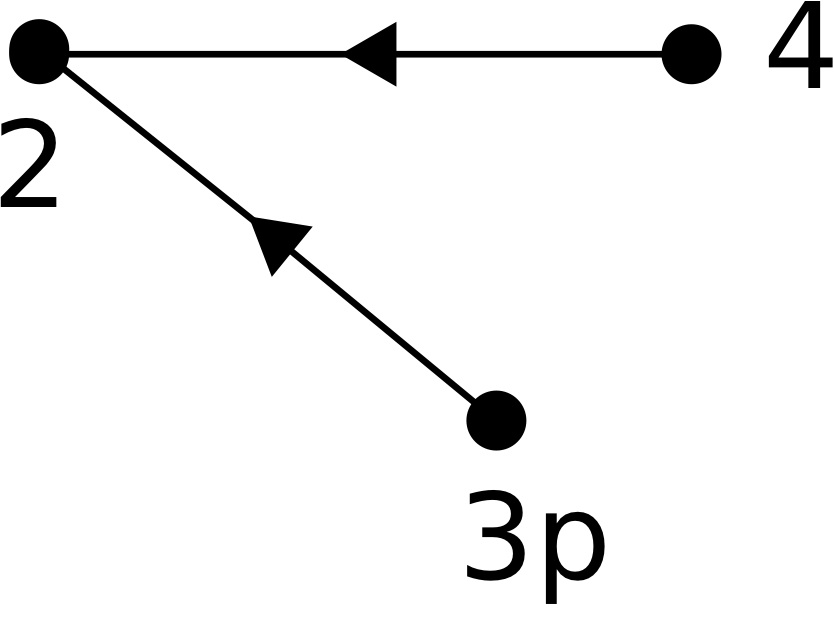
\includegraphics[width=0.15\textwidth]{Hopf.jpg}
\caption{A component of the graph of $f$-homotopy for Hopf surfaces.}
\label{Hopffig}
\end{figure}
\end{example}

\begin{remark}
Using the five classes of Hopf surfaces, one obtains a graph of small deformations which is more precise and complicated than the graph of $f$-homotopy, see \cite[p.\,31]{We}. The graph of $f$-homotopy must be considered as a very rough decomposition of $\cI$.
\end{remark}

\begin{example}[Hirzebruch surfaces]
\label{Hirzebruch}
Consider $X=\mathbb S^2\times\mathbb S^2$. It admits complex structures of even Hirzebruch surfaces $\mathbb F_{2a}$. By \cite{F-Q}, this exhausts the set of complex surfaces diffeomorphic to $X$. Then there is only one connected component of complex structures up to action of the mapping class group. The mapping class group is not known (\cf footnote \ref{Hatcher}) but contains at least four elements generated by
\[
f(x,y)=(a(x),a(y))\quad\text{ and }\quad g(x,y)=(y,x).
\]
where $a$ is the antipodal map of $\mathbb S^2$. Analogously to Lemma \ref{Hopfcc} and Corollary \ref{Hopfcc2}, we have
\begin{lemma}
\label{Hirzebruchcc}
Let $\phi$ be a diffeomorphism of $X$. Assume that $\phi$ leaves a connected component of $\cI$ invariant. Then $\phi$ is $C^\infty$-isotopic either to $g$ or to the identity.
\end{lemma}

\begin{proof}
Let $J_0$ represent $\mathbb P^1\times\mathbb P^1$.
Assume that $J_0\cdot \phi$ belongs to the same connected component as $J_0$. Then there exists a $c$-homotopy of Hirzebruch surfaces \hbox{$\pi : \mathcal X\!\to\![0,1]$} with endpoints $X_0$ and $X_{J_0\cdot \phi}$: just take the tautological family above a smooth path in $\cI$ joining $J_0$ to $J_0\cdot f$. By \cite[Th.\,8.1]{circle}, there exists an analytic space $K$ encoding the complex structures on a neighborhood of the path and obtained by gluing together a finite number of Kuranishi spaces of Hirzebruch surfaces (up to taking the product with some vector space) such that the family $\pi$ maps onto a smooth path into $K$. Using the description of the Kuranishi spaces of Hirzebruch surfaces in \cite[p.\,21]{Cat} (see also Example \ref{Hirzebruchbis}), it is easy to check that
\begin{enumerate}
\item
$K$ is a manifold,
\item
the points of $K$ encoding $\mathbb F_{2a}$ for $a>0$ belongs to a submanifold of complex codimension at least $1$.
\end{enumerate}
Hence, we may replace the initial path defining the $c$-homotopy with a new path and a thus a new $c$-homotopy with same endpoints and such that all surfaces along this path are biholomorphic to $\mathbb P^1\times\mathbb P^1$. By Fischer-Grauert's theorem (see \cite{PS} for the version we use), such a deformation is locally trivial, hence trivial since the base is an interval, \ie there exists a smooth isotopy of biholomorphisms
\begin{equation}
\label{isotopy}
\psi_t\ :\ \mathbb P^1\times\mathbb P^1\to \pi^{-1}(t)\quad (t\in [0,1]).
\end{equation}
In particular, $\psi_1\circ\psi_0^{-1}$
induces a biholomorphism between $X_0$ and $X_{J_0\cdot\phi}$, which is smoothly isotopic to the identity. Composing its inverse with $\phi$, this gives an automorphism of $X_0$, that is, of $\mathbb P^1\times\mathbb P^1$, which corresponds to the same element of the mapping class group as $\phi$. Comparing with the automorphism group of $\mathbb P^1\times\mathbb P^1$ yields the result.
\end{proof}

\begin{corollary}
\label{Hirzebruchcc2}
The map \eqref{mccc} is surjective with kernel $\{[\Id], [g]\}$.
\end{corollary}

\begin{proof}
Since all Hirzebruch surfaces are $c$-homotopic, \eqref{mccc} is surjective. Lemma \ref{Hirzebruchcc} gives the kernel.
\end{proof}

Now, fix a connected component $\cI_0$. We want to describe it more precisely. Observe that $g$ corresponds to an automorphism of $\mathbb P^1\times\mathbb P^1$, but not of the other Hirzebruch surfaces since every automorphism of $\mathbb F_{2a}$ is isotopic to the identity for $a>0$. Recall that the dimension of the group of automorphism of $\mathbb F_{2a}$ is $2a+5$ for $a>0$, \cite[p.\,44]{MK}. This implies
\begin{lemma}
\label{gaction}
We have:
\begin{enumerate}
\item\label{gaction1}
The subset $\cI_0(\mathbb F_0)$ of $\cI_0$ consisting of structures biholomorphic to $\mathbb P^1\times\mathbb P^1$ is open and connected.
\item\label{gaction2}
The closed set $\cI_0\setminus \cI_0(\mathbb F_0)$ has exactly two connected components.
\item\label{gaction3}
The diffeomorphism $g$ acts on $\cI_0$ by fixing globally $\cI_0(\mathbb F_0)$; and by exchanging the two components of $\cI_0\setminus \cI_0(\mathbb F_0)$.
\item\label{gaction4}
Fix a connected component $\cI_1$ of $\cI_0\setminus \cI_0(\mathbb F_0)$. Then the set of points $\cI_2$ encoding $\mathbb F_2$ in $\cI_1$ is open and connected and its complement is connected.
\item\label{gaction5}
By induction, for $a>1$, the set of points $\cI_a$ encoding $\mathbb F_{2a}$ in $\cI_{a-1}$ is open and connected and its complement is connected.
\end{enumerate}
\end{lemma}

\begin{proof}
Observe that $\cI_0(\mathbb F_0)$ is equal to $\cI_0(7)$, recall \eqref{I(k)}. Hence it is open. Also we have already observed in the proof of Lemma \ref{Hirzebruchcc} that two $c$-homotopic structures both encoding $\mathbb P^1\times\mathbb P^1$ are $c$-homotopic through a path all of whose points encode $\mathbb P^1\times\mathbb P^1$. This proves \eqref{gaction1}.

To prove \eqref{gaction2} and \eqref{gaction3}, we need a variation of Lemma \ref{Hirzebruchcc}. Let $J_0$ represent $\mathbb F_2$. Call~$\cI_1$ the connected component of $J_0$ in $\cI_0\setminus \cI_0(\mathbb F_0)$.
Assume that $J_0\cdot\phi$ belongs to~$\cI_1$. Then there exists a smooth family of Hirzebruch surfaces $\pi : \mathcal X\to [0,1]$ with endpoints $X_0$ and $X_{J_0\cdot\phi}$ and all of whose point are distinct from $\mathbb P^1\times\mathbb P^1$. Using \cite[Th.\,8.1]{circle} and the description of the Kuranishi spaces of Hirzebruch surfaces in \cite[p.\,21]{Cat} (see also Example \ref{Hirzebruchbis}), it is easy to check that
we may assume that all surfaces along this path are biholomorphic to $\mathbb F_2$. Arguing as in the proof of Lemma \ref{Hirzebruchcc}, we deduce that $\phi$ must be smoothly isotopic to the identity, since every automorphism of $\mathbb F_2$ has this property. Since we already know that $g$ fixes globally $\cI_0$, this means that $J_0$ and $J_0\cdot g$ belongs to two distinct connected components of $\cI_0\setminus \cI_0(\mathbb F_0)$ in $\cI_0$.\enlargethispage{.5\baselineskip}%

Assume now that $J_1$ is another point of $\cI_0$ encoding $\mathbb F_2$. Then there exists $\phi\in\Diff^+(X)$ such that $J_1$ equals $J_0\cdot\phi$. By Corollary \ref{Hirzebruchcc2}, $\phi$ is either isotopic to the identity or to $g$. In the first case, $J_1$ belongs to also to $\cI_1$. In the second case, it~belongs to $\cI_1\cdot g$. Hence, there are exactly two connected components exchanged by~$g$, and items \eqref{gaction2} and \eqref{gaction3} are proved.

Finally, similar arguments prove\eqref{gaction4} and \eqref{gaction5}.
\end{proof}
\end{example}

In other words, the associated graph of $f$-homotopy has several connected components and each connected component has two branches joined on the vertex corresponding to $\mathbb P^1\times\mathbb P^1$. Finally, each branch has a countable number of vertices, namely one vertex for each value of $a\in\mathbb N$. It has weight $2a+5$, except for $\mathbb F_0$ which has weight $6$. Given any $a>b$, there exists an edge from $a$ to $b$, because it is possible to deform $\mathbb F_{2a}$ onto $\mathbb F_{2b}$, \cf \cite{Cat} or \cite{MK}. In particular, every vertex is attached to a countable number of edges. Similar picture is valid for the odd Hirzebruch surfaces.
\begin{figure}[htb]
\centering
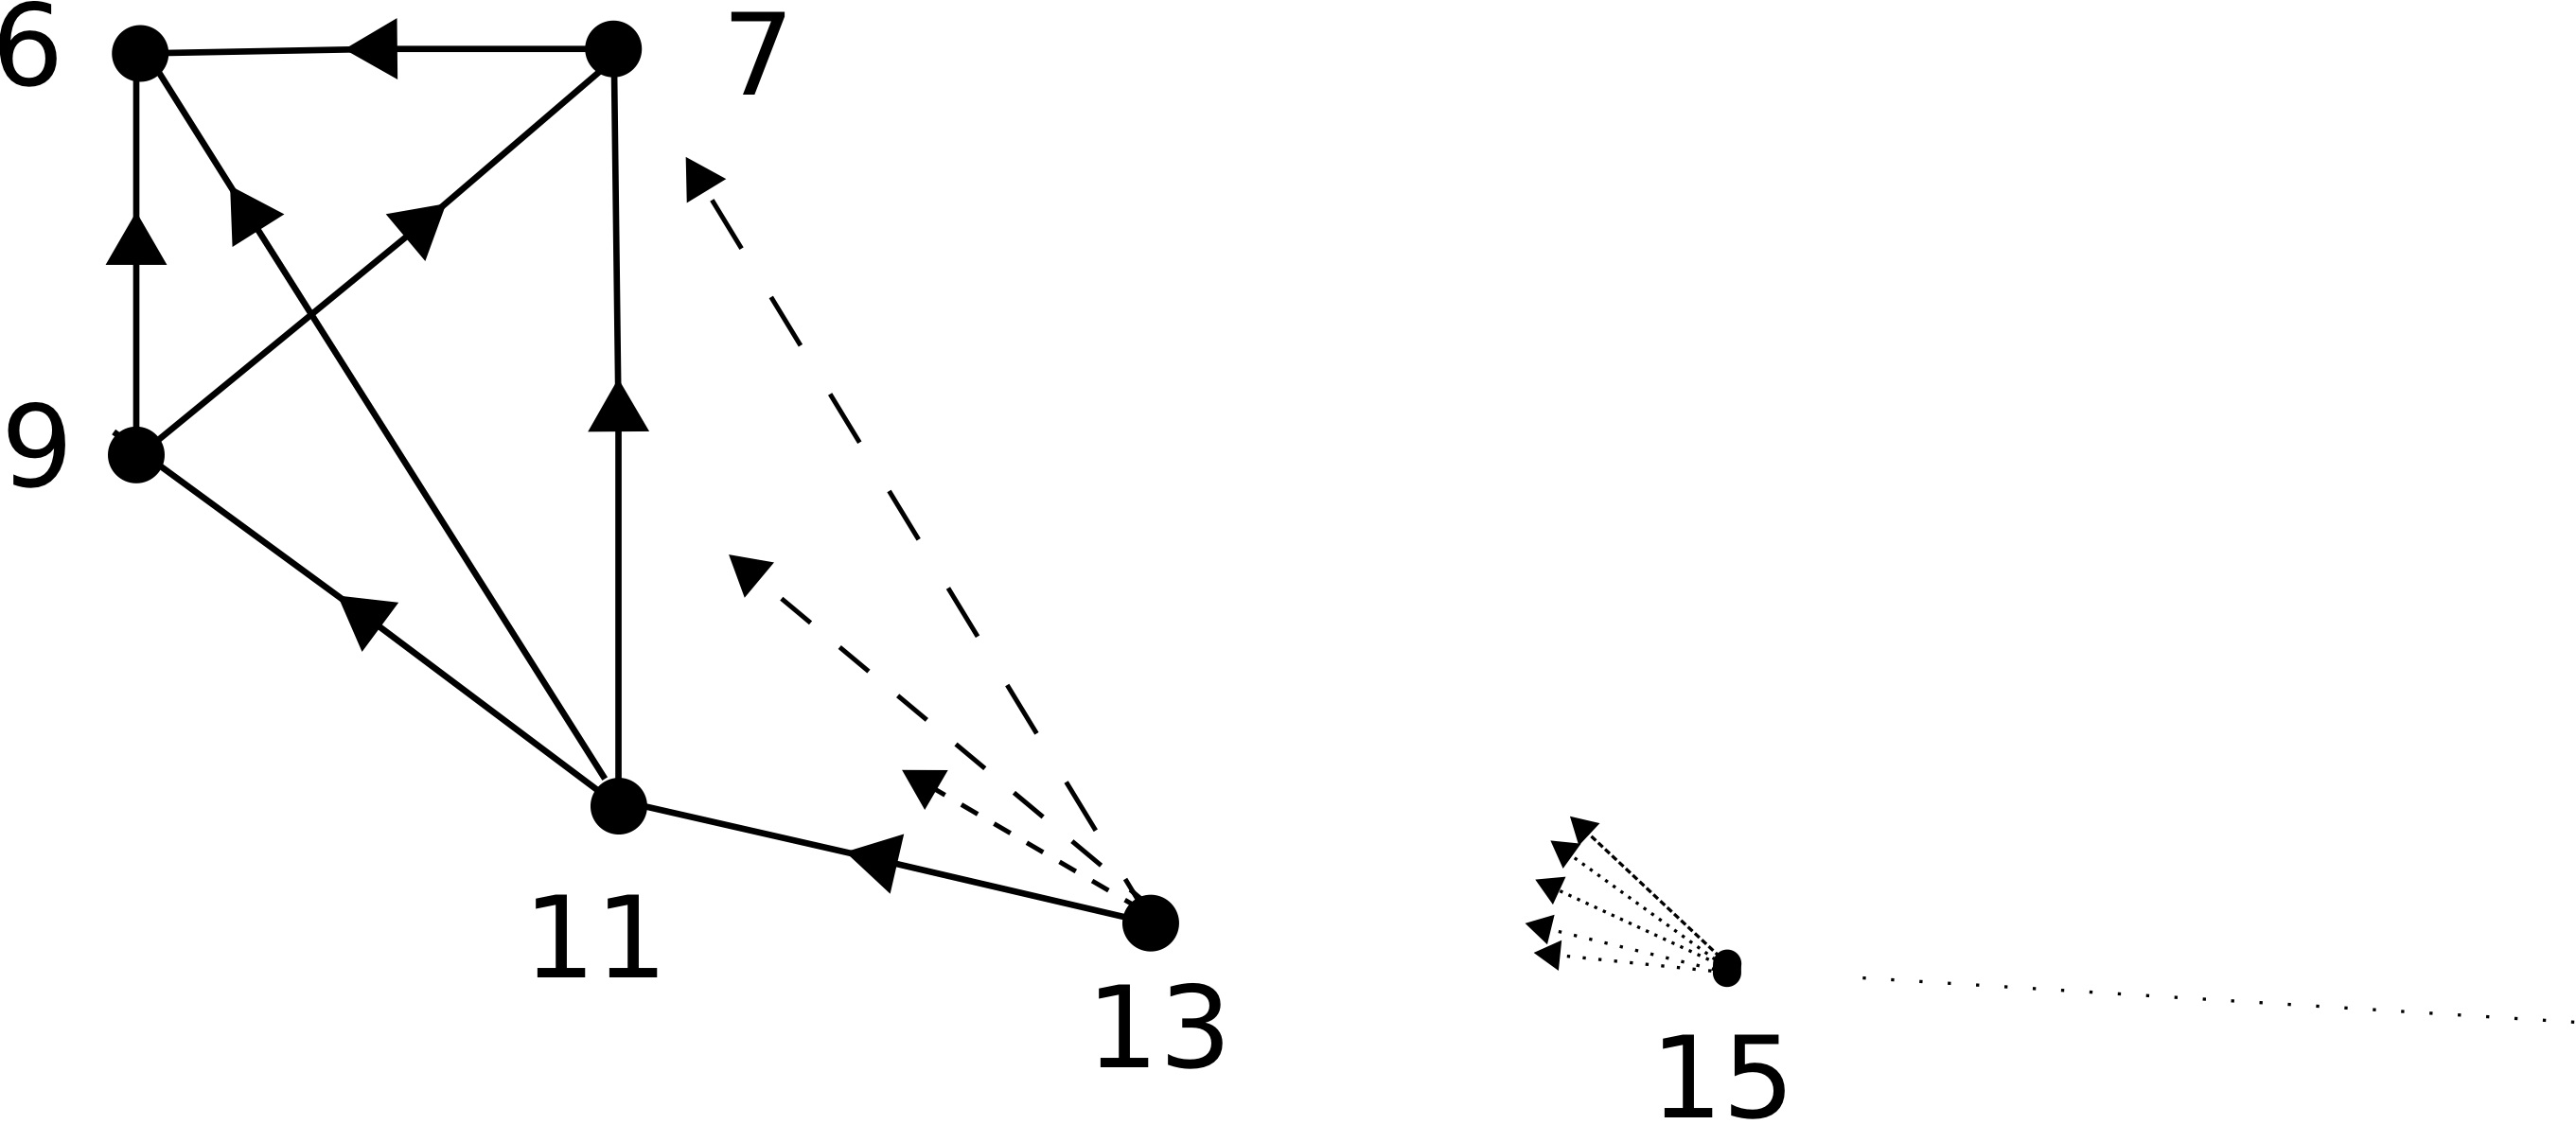
\includegraphics[width=0.45\textwidth]{Hirzebruch}
\caption{One of the two branches of a component of the graph of $f$-homotopy for Hirzebruch surfaces.}
\label{Hirzebruchfig}
\end{figure}

\begin{remark}
\label{ell}
Observe that the action of the mapping class group on $\cI$ may take strongly different forms, depending on the $C^\infty$-manifold $X$. For $\mathbb S^3\times\mathbb S^1$, Lemma~\ref{Hopfcc} shows that it only permutes the connected components of $\cI$. For $\mathbb S^2\times \mathbb S^2$, some of the elements of the mapping class group permute the connected components of~$\cI$ but we also have by Lemma \ref{gaction} an involution which fixes each component of~$\cI$. Note that this involution is isotopic to an automorphism of $\mathbb P^1\times\mathbb P^1$. The case of elliptic curves shows a different phenomenon. There is a single connected component of complex structures which is fixed by every element of the mapping class group $\SL_2(\mathbb Z)$. Some of them are isotopic to an automorphism of an elliptic curve, for example the multiplication by $i$; but most of them are not, \cf Example \ref{tori}.
\end{remark}

\begin{remark}
\label{CC2}
Observe that in Examples \ref{Hopf} and \ref{Hirzebruch}, the Riemann moduli space $\mathcal M^s(X)$ is connected because of Lemmas \ref{Hopfcc} and \ref{Hirzebruchcc} (\cf Remark \ref{countableexamples}). However, we do not know if $\mathcal T^s(X)$ has a finite number of connected components, because it is not known if the mapping class group of $\mathbb S^1\times\mathbb S^3$, respectively $\mathbb S^2\times\mathbb S^2$, is finite or not.\footnote{I owe this information to Daniel Ruberman.} For example, notice that some blow ups of connected sums of $\mathbb P^2$s have infinite mapping class group, see \cite{Ruber}.
\end{remark}

\section{The TG foliated structure of \texorpdfstring{$\cI$}{I} and its holonomy groupoid}
\label{TGfoliationsection}
Let $\cI_0$ be a connected component of $\cI$. The connected group $\D$ fixes $\cI_0$ and we want to show that the action of $\D$ induces a foliated structure on $\cI$.

Let us review a very classical situation when a group action induces a foliation. Assume that a finite-dimensional complex Lie group $G$ acts analytically onto a finite-dimensional complex manifold $M$. Assume that the action is locally free, that is, given any $x\in M$, there exists some neighborhood $U$ of the identity in $G$ such that the following property is true for any $g\in G$\vspace*{-2pt}
\begin{equation*}
x\cdot g=x\quad\Longrightarrow \quad g\not\in U.
\end{equation*}
Then the orbits of the $G$-action foliates holomorphically $M$ \cite[\S 2.1]{CLN}. The proof exhibits a foliated atlas. In fact, let $e$ denote the neutral element of $G$ and $\mathfrak G$ its Lie algebra. Each point $x\in M$ has a neighborhood $W$ homeomorphic to a neighborhood $V$ of $(e,0)$ in the product of $\mathfrak G$ with some $\CC^p$; if we denote this homeomorphism by $\phi$, then $\phi$ sends the intersection of a $G$-orbit with $W$ onto a plaque $V\cap (\mathfrak G\times\{\text{Cst.}\})$; and $\phi^{-1}$ sends $V\cap (\{e\}\times\CC^p)$ onto a local transverse, that is, a submanifold which meets transversally the orbits. Moreover, the changes of charts are holomorphic and foliated, which means that they preserve the plaques. The leaves are the orbits. They acquire a structure of complex manifold and immersed submanifolds of $M$. Observe that the isotropy groups of a locally free action are discrete.

In our situation, the isotropy groups are not discrete, except for the following case.

\begin{proposition}
\label{foliationsimple}
Assume that the function $h^0$ is identically zero on the connected component $\cI_0$. Then,
\begin{enumerate}
\item\label{foliationsimple1}
the action of $\Diff^0(X)$ onto $\cI_0$ is locally free,
\item\label{foliationsimple2}
the orbits of the $\Diff^0(X)$ action onto $\cI_0$ induces a holomorphic foliation of~$\cI_0$.
\end{enumerate}
\end{proposition}

Here, by inducing a foliation of $\cI_0$, we mean: every point $J$ of $\cI_0$ has a neighborhood which is locally isomorphic\footnote{Recall Convention \ref{ConvFrH}.} to the product of a Fréchet manifold with the Kuranishi space of $X_J$ and whose local transverse section at a point $J$ is given by the Kuranishi space of $X_J$; the orbits are Fréchet manifolds and submanifolds of $\cI_0$ in the weak sense that there exists an injective analytic immersion of each leaf in $\cI_0$; they are locally sent to the plaques; the changes of charts are analytic and foliated.

\begin{remark}
\label{foldef}
Be careful that we use the word ``foliation'' in an extended sense. Firstly the leaves are infinite-dimensional and secondly the transverse sections are singular spaces and are not all isomorphic. We should rather talk of ``lamination'' but we prefer to reserve this terminology for foliated spaces transversely modeled onto a continuous space, \eg a Cantor set.
\end{remark}

\begin{proof}
Pass to Sobolev classes. The condition that the function $h^0$ is zero on the whole $\cI$ and thus on $(\cI_l)_0$ by upper semi-continuity implies that, in Theorem \ref{KuranishiTheorem}, we may take $L_0$ to be the full $A^0_{l+1}$. This complex vector space is, as a real vector space, the space of vector fields $\Gamma_{l+1}(TX)$. Its complex structure a priori depends on the base point $J$, but it is easy to check that all $A^0_{l+1}$ are isomorphic as complex vector spaces, \cite[Lem.\,7.1]{circle}. Hence the isomorphisms \eqref{Phi0} form an analytic foliated atlas of $(\cI_l)_0$: the plaques representing the local orbits of $\Diff^0_{l+1}(X)$ are preserved by the changes of charts, \cf \cite[\S 6]{circle}. The plaques are Hilbert manifolds modeled onto $A^0_{l+1}$ and analytically embedded in $(\cI_l)_0$. Since the changes of charts are analytic and foliated, plaques of the same orbit are gluing together to give a Hilbert manifold structure on the corresponding orbit, and an analytic immersion into $(\cI_l)_0$. At a point $J$, any germ of transverse section is isomorphic to the Kuranishi space of $X_J$. Recalling Convention \ref{ConvFrH} and Remark \ref{rkFrechetHilbertchart}, we obtain \eqref{foliationsimple2}. Finally the action is locally free by \eqref{Kuranishiaction}, so \eqref{foliationsimple1} is also proved.
\end{proof}

In the general case, we think of Kuranishi theorem \ref{KuranishiTheorem} as describing a foliated structure on $\cI$ with analytic orbits and which is no more transversally modeled onto an analytic space as in Proposition \ref{foliationsimple} but on the Kuranishi stack of Section \ref{localaction}. In previous versions of this paper, we formalize this structure as a TG foliation, but the definition we gave is not completely satisfactory. There are several technical issues with it and solving them is unrelated to our results, so we prefer replacing it with the notion of TG foliated structure which is a purely transverse notion.\enlargethispage{-\baselineskip}%

\begin{definition}
\label{tgfoldef}
By \emph{TG foliated structure of $\cI$}, we mean a collection of Kuranishi stacks associated to a collection of Kuranishi domains which cover the whole space~$\cI$.
\end{definition}
We think of it as a collection of local transversals to the $\D$-action.

\begin{remark}
\label{rkTG}
TG stands for transversely in groupoids. It highlights the fact that the local transversals are not manifolds or analytic spaces but stacks, and thus encoded in a groupoid.
\end{remark}

We now want to define and encode the holonomy of these local transversals. Let us first review how it works for a classical foliation.

So, let $\mathcal F$ be a foliation of some complex manifold. We may associate to it a holonomy groupoid as follows (\cite[\S 5.2]{Moerdijk} and \cite{Ha}). We choose a set of local transverse sections. Objects of the groupoid are points of the disjoint union of these local sections. Morphisms are generated by holonomy morphisms, obtained by following the leaves from a transverse section to another one, identifying holonomy morphisms having the same germ. It is an étale analytic groupoid, which encodes analytically the leaf space of the foliation: its geometric quotient is homeomorphic to the leaf space and its analytic structure reflects the analyticity of the initial foliation.

Having proved in Proposition \ref{foliationsimple} that the action of $\Diff^0(X)$ induces a foliation of each connected component of $\cI$ when $h^0$ is equal to zero, and considering in the general case the TG foliated structure of $\cI$, we would like to associate to this TG foliated structure a holonomy groupoid. As in the classical case, it should be analytic; and its geometric quotient should be isomorphic to the leaf space. Later on, we will show that is also a presentation of the Teichmüller stack.

However, this is much more involved than in the classical case. The problem is that now the transverse sections are modeled onto groupoids \eqref{tgdef}, so that holonomy morphisms are stacks morphisms between Kuranishi stacks. Hence, if we just follow the same strategy, instead of building a groupoid, we end with a disjoint union of stacks and a set of local stack morphisms. It is certainly possible to turn this collection into a nice categorical structure. However, we will not follow this path since we are interested in obtaining a presentation of the Teichmüller stack. The crucial point is to lift holonomy morphisms between Kuranishi stacks to morphisms between Kuranishi spaces. This lifting process will be done in four steps, in Sections \ref{multifoliate}, \ref{Teichmueller} and \ref{main}.

Firstly in Section \ref{multifoliate}, we construct partial foliations of $\cI_0$. Partial here means that they are not defined on the whole $\cI_0$ but on an open subset. We take a countable collection of such foliations whose domains of definition cover $\cI_0$. Basically, the transverse structure of these foliations at some point $J$ is modeled onto the Kuranishi space of the corresponding complex manifold $X_J$. However, the jumps in the dimension of the automorphism group cause serious problems here, and we start doing the construction in the neighborhood of a $f$-homotopy class, where equidimensionality is fulfilled. Then we extend it to the whole $\cI_0$, but to achieve that, we are forced to fat the smallest Kuranishi spaces to finish with all transversals of the same dimension. This fattening process was already used in \cite{circle}.

Secondly, from this set of partial foliations, we define regular atlases for this multifoliation and simple holonomy germs as the classical holonomy germs of each partial foliation. The main point is that we allow, under certain circumstances, composition of holonomy germs coming from two different foliations. The peculiarities of a regular atlas are useful in this process. We encode all the holonomy data related to a regular atlas in a groupoid. This is however not the good groupoid to consider, especially because changing of regular atlas does not produce a Morita equivalent groupoid. All~this is done in Sections \ref{regatlas}, \ref{simpleholonomy} and \ref{firstapp}. This preliminary work is essentially notational and technical, but is important to achieve the construction.

Thirdly, building on the previous sections, we construct in Section \ref{Teichsub} the holonomy groupoid of the TG foliated structure of $\cI_0$. We call it the \emph{Teichmüller groupoid}. Its objects are points of a disjoint union of transverse sections of partial foliations covering~$\cI_0$. Its morphisms are composition of the simple holonomy germs and of morphisms of type \eqref{Aut0action} on its Kuranishi space, up to an equivalence relation.

Fourthly, and last, we prove that the Teichmüller groupoid is an analytic smooth groupoid and a presentation of the Teichmüller stack in Theorem \ref{maintheorembis}, which implies Theorem \ref{maintheorem}. Basically there are two points to check. From the one hand, it must be shown that composition of simple holonomy germs and local automorphisms describes the full action of $\Diff^0(X)$ onto $\cI_0$. This is done in Lemma \ref{isoteich}. As a consequence, its geometric quotient is homeomorphic to $\mathcal T^s(X,\cI_0)$. From the other hand, it must be shown that the source and target maps are smooth morphisms. This is essentially an adaptation of the arguments involved in the proof of Lemma \ref{analyticKurstack}. Analogously, we prove Theorem \ref{mainRbis}, which implies Theorem \ref{mainR}.

Before developing all this construction, we consider in the next section the rigidified case, in which the TG foliated structure comes from a foliation, and the Teichmüller groupoid an ordinary holonomy groupoid. This can be seen as a toy model for the general construction and will serve to fixing some notations and conventions.

\section{The rigidified case}
\label{rigidified}

Recall \eqref{Aut1} and

\begin{definition}[see {\cite[Def.\,12]{Catsurvey}}]
\label{rig}
A compact complex manifold $X_J$ is \emph{rigidified} if $\Aut^1(X_J)$ is equal to the identity. More generally, we say that a subset $V$ of~$\cI$ is rigidified if $X_J$ is rigidified for all $J\in V$.
\end{definition}

In that case, the map
\begin{equation}
\label{injorbit}
f\in\Diff^0(X)\mto J\cdot f\in\cI
\end{equation}
is injective. Moreover, the following holds.

\begin{proposition}
\label{rigidconsequences}
Assume that all structures of some connected component $\cI_0$ are rigidified. Then, the action of $\Diff^0(X)$ onto $\cI$ is free and defines a foliation of $\cI_0$ whose leaves are Fréchet manifolds modeled onto the vector space of smooth sections of $TX$ and with local transversal $K_0$ at $J_0$.
\end{proposition}

\begin{proof}
Freeness is immediate from \eqref{injorbit}. The foliation is that of Proposition \ref{foliationsimple}.
\end{proof}

In the case of Proposition \ref{rigidconsequences}, the Teichmüller groupoid is just the standard holonomy groupoid of the foliation. We give now a complete treatment of this case, which serves as a toy model for Section \ref{Teichmueller}. We cover $\cI_0$ by a collection $(U_\alpha)_{\alpha\in A}$ of open subsets. We assume that each chart $U_{\alpha}$ is a Kuranishi domain satisfying hypothesis \ref{squarehyp} associated to the following retraction map (the composition is the identity, \cf \eqref{id})%
\begin{equation}
\label{id2rigid}
K_{\alpha}\hto U_{\alpha}\To{\Xi_{\alpha}}K_{\alpha}.
\end{equation}
We denote by $J_\alpha$ the base point of the Kuranishi space $K_\alpha$. Observe that the index set may be assumed to be countable, due to Proposition \ref{countableTeich} and the countability of the involved topologies.

Take two points $x\in K_\alpha$ and $y\in K_\beta$ belonging to the same leaf and choose a path of foliated charts joining $x$ to $y$. A holonomy germ from $x$ to $y$ is a germ of analytic isomorphism between the pointed spaces $(K_\alpha,x)$ and $(K_\beta,y)$, which is obtained by identifying along the path of foliated charts points belonging to the same leaf, see \cite[\S 2.1]{Moerdijk} or \cite{CLN}.

They can be encoded in a holonomy groupoid \cite[\S 5.2]{Moerdijk} or \cite{Ha} as follows. \emph{Objects} are points of the disjoint union of transversals
\begin{equation}
\label{objectshg}
\uniondisjointe_{\alpha\in A} K_\alpha.
\end{equation}
We denote by $(x,\alpha)$ a point of $K_\alpha$. To encode the morphisms, we first notice that on each non-empty intersection $U_{\alpha}\cap U_{\beta}$, there exists a unique isomorphism $\phi_{\alpha,\beta}$ between some open subset $K_{\alpha, \beta}$ of $K_{\alpha}$ and some open subset $K_{\beta, \alpha}$ of $K_{\beta}$. It is obtained by following the leaves of the foliation from $K_{\alpha}$ till meeting $K_{\beta}$ (when this occurs). It satisfies the commutative diagram\vspace*{-3pt}
\begin{equation}
\label{CDhol}
\begin{tikzcd}
U_{\alpha}\cap U_{\beta} \arrow[d,"\Xi_{\alpha}"']\arrow[r,"\Id"] &U_{\alpha}\cap U_{\beta}\arrow[d,"\Xi_{\beta}"]\\
K_{\alpha,\beta}\arrow[r,"\simeq","\phi_{\alpha,\beta}"'] &K_{\beta,\alpha}
\end{tikzcd}
\end{equation}

\begin{remark}
\label{reducedrigidified}
It happens that Kuranishi spaces are everywhere non-reduced. Hence a morphism between Kuranishi spaces is not completely determined by its values, the values of its differential must also be prescribed. The previous definition of $\phi_{\alpha,\beta}$ by following the leaves just determines its values. However, since $\Xi_\alpha$ and $\Xi_\beta$ are smooth morphisms by Kuranishi's theorem \ref{KuranishiTheorem}, hence locally trivializable on the source, \cf \eqref{flatness}, it is also uniquely defined in the non-reduced case.
\end{remark}

We now look at the groupoid of germs generated by the $\phi_{\alpha,\beta}$, \cf \cite[1.2]{Ha}. In other words, we now let $(\alpha_1,\hdots,\alpha_n)$ be a collection of indices such that each $U_{\alpha_i}\cap U_{\alpha_{i+1}}$ is non-empty and define\vspace*{-3pt}
\begin{equation}
\label{phialpha1n}
\phi_{\alpha_1,\hdots,\alpha_n}:=\phi_{\alpha_{n-1},\alpha_n}\circ\cdots\circ \phi_{\alpha_1,\alpha_2}.
\end{equation}
This composition is defined on some open subset of $K_{\alpha_1}$ that we denote by $K_{\alpha_1,\hdots,\alpha_n}$; and it ranges in some open subset of $K_{\alpha_n}$, that we denote by $K_{\alpha_n,\hdots, \alpha_1}$. Then we represent all holonomy maps as
points of
\begin{equation}
\label{morphismholonomyrigidified}
\uniondisjointe_{n\geq 1}\biggl (\uniondisjointe_{(\alpha_1,\hdots,\alpha_n) \in B_{n}} K_{\alpha_1,\hdots,\alpha_n}\biggr ).
\end{equation}
Here $(\alpha_1,\hdots,\alpha_n) \in B_{n}$ if each $U_{\alpha_i}\cap U_{\alpha_{i+1}}$ is non-empty.
A point $x$ in some $K_{\alpha_1,\hdots,\alpha_n}$ represents the germ at $x$ of the map $\phi_{\alpha_1,\hdots,\alpha_n}$, the case $n=1$ encoding the identity
germs. We denote such a point by the $(n+1)$-uple $(x,\alpha_1,\hdots,\alpha_n)$.

Consider the groupoid whose objects are given in \eqref{objectshg}, and morphisms are given in \eqref{morphismholonomyrigidified}. Observe that both sets are $\CC$-analytic spaces. The source map sends $(x,\alpha_1,\hdots, \alpha_n)$ onto $(x,\alpha_1)$ and the target map sends it to $(\phi_{\alpha_1,\hdots,\alpha_n}(x),\alpha_n)$. Both are obviously étale analytic maps, since the source map is just the inclusion $K_{\alpha_1,\hdots,\alpha_n}\subset K_{\alpha_1}$ on the component $K_{\alpha_1,\hdots,\alpha_n}$;\footnote{This component has no reason to be connected.} and the target map on the same component is the composition of the isomorphism $\phi_{\alpha_1,\hdots,\alpha_n}$ from $K_{\alpha_1,\hdots,\alpha_n}$ onto $K_{\alpha_n,\hdots,\alpha_1}$ with the inclusion $K_{\alpha_n,\hdots,\alpha_1}\subset K_{\alpha_n}$. Multiplication is given by composition of holonomy germs.

However, we are not finished yet. The previous groupoid is not the holonomy groupoid of the foliation. We must still identify identical germs. It may happen for example that such a composition $\phi_{\alpha_1,\hdots,\alpha_n}$ is the identity. So we take the quotient of \eqref{morphismholonomyrigidified} by the following equivalence relation
\begin{equation}
\label{equivrigid}
(x,\alpha)\sim (x',\alpha')\iff
\left\{
\begin{aligned}
&x=x',\ \alpha_1=\alpha'_1,\ \alpha_n=\alpha'_{n'}\cr
\text{and }&\big (\phi_{\alpha_1,\hdots,\alpha_n}\big )_{x'}\equiv \big (\phi_{\alpha'_1,\hdots,\alpha'_{n'}}\big )_x,
\end{aligned}
\right .
\end{equation}
that is, if they have same source, same target, and are equal as germs.
Hence, the set of morphisms is
\begin{equation}
\label{morphismholonomyrigid2}
\uniondisjointe_{n\geq 1}\biggl (\uniondisjointe_{(\alpha_1,\hdots,\alpha_n) \in B_{n}} K_{\alpha_1,\hdots,\alpha_n}\biggr )\biggm /\sim.
\end{equation}

\begin{definition}
\label{teichrigid}
Assume that $\cI_0$ is rigidified. We call \emph{Teichmüller groupoid} of $\cI_0$ the groupoid whose objects are given by \eqref{objectshg}, whose morphisms are given in \eqref{morphismholonomyrigid2}, and whose source, target maps and multiplication are defined as above.
\end{definition}
We define in the same way the Teichmüller groupoid of $V$, an open subset of $\cI$. We emphasize that this definition is valid only if $V$ is rigidified. The general definition of Teichmüller groupoid will be given in Section \ref{Teichmueller}.

\begin{proposition}
\label{groupoidrigid}
The Teichmüller groupoid of a rigidified subset $V$ of $\cI$ is an analytic étale groupoid.
\end{proposition}

\begin{proof}
From the above discussion, we just have to prove that \eqref{morphismholonomyrigid2} is still an analytic space and that the projection map from \eqref{morphismholonomyrigidified} onto \eqref{morphismholonomyrigid2} is étale.

Observe that two distinct points of the same component $K_{\alpha_1,\hdots,\alpha_n}$ of \eqref{morphismholonomyrigidified} cannot be equivalent. Therefore, the natural projection
map from \eqref{morphismholonomyrigidified} onto \eqref{morphismholonomyrigid2} is étale and we just have to show that \eqref{morphismholonomyrigid2} is Hausdorff to finish with the proof.

This comes from a standard argument, \cf \cite[Prop.\,3.2]{Brunella}. Consider two equivalent convergent sequences $(x_p,\alpha_p)$ and $(x_p, \alpha'_p)$. We may assume that all $\alpha_p$, \resp $\alpha'_p$, are the same, say $\alpha$, \resp $\alpha'$. Assume that $(x_p)$ converges to $x$. Then this means that $\big (\phi^{-1}_{\alpha_1,\hdots,\alpha_n}\circ \phi_{\alpha'_1,\hdots,\alpha'_n}\big )_{x_p}\equiv \Id_{x_p}$, \ie the germ of this morphism is the identity at every point $x_p$. By analyticity, this implies that it is also the identity at the limit point $x$.
\end{proof}

\begin{remark}
\label{moritaequivrigid}
The construction above depends on a choice of a foliated atlas. However, it is easy to show that it is independent of this choice up to Morita equivalence. This can of course be deduced afterward from general arguments, since we will show in Theorem \ref{maintheorembis} that its stackification is isomorphic to the stack $\mathcal T(X,\cI_0)$, which does not depend on a foliated atlas. It can also be proved directly as follows. Start with a foliated atlas and construct the associated Teichmüller groupoid. Take a finer foliated atlas. Then the associated Teichmüller groupoid is just the localization of the first one over the new atlas, hence both are weakly equivalent \cite{Ha}. Start now with two different foliated atlases and their associated Teichmüller groupoid. Since the union of the atlases is a common refinement of both of them, the two groupoids are Morita equivalent.
\end{remark}

\begin{remark}
\label{Aut10bis}
Assume that for all structures $J$ in $\cI_0$, we have $\Aut^0(X_J)$ equal to the identity. Then Proposition \ref{foliationsimple} still applies and the action of $\Diff^0(X)$ still defines a foliation of $\cI_0$. So we can still define a holonomy groupoid as above. Moreover the geometric quotient of the Teichmüller stack equals the leaf space, that is, the geometric quotient of this holonomy groupoid. Nevertheless, they may be different as \emph{stacks}, because there may exist a non trivial element in $\Aut^1(X_J)$ that fixes $\cI_0$. Such an element is encoded in the Teichmüller groupoid we construct in Section \ref{Teichmueller} but not in the holonomy groupoid constructed in this section, \cf Remark \ref{subtle}. This explains why we assume that $\cI_0$ is rigidified in Definition \ref{teichrigid}.

For many compact complex manifolds $X_0$, there is no difference between $\Aut^0(X_0)$ and $\Aut^1(X_0)$, \cf \cite{Catsurvey}. We gave an example of $X_0$ with $\Azero$ and $\Aun$ distinct in \cite{Aut1paper}. The dimension of $\Azero$ is positive so this leads to the following problem.

\begin{problem}
Find a compact complex manifold $X_0$ with $\Aut^0(X_0)$ being reduced to the identity but which is not rigidified.
\end{problem}

If $X_0$ is Kähler, then a result of Liebermann implies that $\Aut^0(X_0)$ has finite index in $\Aut^1(X_0)$.\footnote{I owe this information to S. Cantat.} In the non-Kähler case, however, there should even exist examples with infinite ``complex mapping class group'' $\Aut^1(X_0)/\Aut^0(X_0)$.
\end{remark}

\section{The set of partial foliated structures of \texorpdfstring{$\cI$}{I}}
\label{multifoliate}

In this section, we associate to the TG foliated structure of a connected component~$\cI_0$ of~$\cI$ a collection of standard foliations of open sets of $\cI_0$ covering it. In Section \ref{simpleholonomy}, we will associate to these partial foliations their holonomy germs. This is a crucial step in defining the morphisms of the Teichmüller groupoid. The main problem here is that the dimension of the Kuranishi spaces may vary inside $\cI_0$. To~overcome this difficulty, we proceed in two steps. It turns out that the dimension we have really to care about in this problem is the dimension of the automorphism group. Hence we first work in the neighborhood of a $f$-homotopy class, so that we may assume equidimension of the automorphism groups involved in the choice of foliated atlases. Then, we treat the general case. We have to fat the Kuranishi spaces with small automorphism group, following a process already used in \cite{circle}. This supposes the function $h^0$ to be bounded on $\cI_0$.

\subsection{The set of partial foliated structures of a neighborhood of a $f$-homotopy class}
\label{multifoliatefclass}
Let $\mathcal F$ be a $f$-homotopy class in $\cI$. Let $V$ be a connected neighborhood of~$\mathcal F$ in $\cI_0$. Let $G(\Sigma(TX))$ be the grassmannian of closed vector subspaces of $\Sigma (TX)$ of codimension $h^0(\mathcal F)$. For each $L\in G(\Sigma (TX))$,
define
\begin{equation}
\label{FL}
\mathcal F_L=\{J\in\mathcal F\mid L\oplus \Re H^0(X_J,\Theta_J)=\Sigma(TX)\}.
\end{equation}

\begin{definition}
\label{Fadmissible}
We say that $L$ is \emph{$\mathcal F$-admissible} if $\mathcal F_L$ is not empty.
\end{definition}

Assume that $L$ is $\mathcal F$-admissible and let $J_0\in\mathcal F_L$. Then, using the isomorphism
\begin{equation}
\label{real}
\xi\in A^0\mto \xi+\bar\xi\in \Sigma (TX)
\end{equation}
(where $A^0$ is the space of $(1,0)$-vectors for the structure $J_0$), we see that the choice of an $\mathcal F$-admissible $L$ is equivalent to the choice of a closed subspace $L_0$ of $A^0$ satisfying~\eqref{A0} and
\begin{equation}
\label{L0L}
\Re L_0=L.
\end{equation}
In the sequel, we will denote by the same symbol $L$ a closed subspace of $A^0$ and its real part in $\Sigma (TX)$. No confusion should arise from this abuse of notation. Observe that all such $L$ are complex isomorphic, \cf \cite[Lem.\,7.1]{circle}.

So, once chosen such an $L$, we may apply Theorem \ref{KuranishiTheorem} at $J_0$ with $L$.
We define~$V_L$ as the maximal open subset of $V$ covered by Kuranishi domains modeled on $L$ and based at points of $\mathcal F_L$. We can interpret it as follows. Theorem \ref{KuranishiTheorem} endows each Kuranishi domain with a trivial local foliation by copies of $L$ and leaf space $K_0$.

Now, let us put this interpretation in a global setting. It tells us that we may cover~$V_L$ by Kuranishi domains modeled on the same $L$.
Hence $L$ defines a foliation of $V_L$ by leaves locally isomorphic to a neighborhood of $0$ in $L$, see \cite[Th.\,7.2]{circle}.\footnote{The assumption of compactness in this theorem is only used to \emph{prove} that there exists a common~$L$ modeling all the Kuranishi domains. Since we assume the existence of such a common $L$, the proof applies.}

\begin{definition}
\label{Lfoliation}
We call this foliation the \emph{$L$-foliation of $V$} (even if it is only defined on $V_L$).
\end{definition}

In the case where $V_L$ is equal to $V$, which is equivalent to saying that $L$ is a common complement to all $H^0(X_J,\Theta_J)$ for $J\in \mathcal F$, then we obtain a global foliation of $V$.

Nevertheless, it is not possible in general to assume this hypothesis. Hence we shall replace this foliated structure by a collection of \emph{partial foliations} encoded in a groupoid.
\begin{definition}
\label{coveringfamily}
A set $\mathcal L$ of $\mathcal F$-admissible elements of $G(\Sigma (TX))$ such that
\begin{equation}
\label{CF}
\bigcup_{L\in\mathcal L} V_L=V
\end{equation}
is called \emph{a covering family} of $V$.
\end{definition}

Choose $\mathcal L$ a covering family of $\mathcal F$. Observe that we may assume $\mathcal L$ to be countable by Proposition \ref{countable1}. To $\mathcal L$ is associated \emph{a covering set of partial foliations} of $V$, defined as the set of all $L$-foliations of $V$ for $L\in\mathcal L$. It is useful to encode it in a groupoid as follows.

For each $L\in\mathcal L$, choose an atlas
\begin{equation}
\label{atlas1}
\mathcal U_L=(U_{\alpha})_{\alpha\in A_L}
\end{equation}
of $V_L$ by $L$-foliated charts satisfying hypothesis \ref{squarehyp}. Define
\begin{equation}
\label{A}
A=\uniondisjointe_{L\in\mathcal L}A_L\quad\text{ and }\quad \mathcal U=(\mathcal U_L)_{L\in\mathcal L}.
\end{equation}

Once again, we may assume that $A$ is countable, due to the countability of the involved topologies. Then define the groupoid $G_{\mathcal U}$ as follows.
\emph{Objects} are points of the disjoint union
\begin{equation}
\label{objects}
\uniondisjointe _{\alpha\in A} U_{\alpha},
\end{equation}
hence are encoded by pairs $(x,\alpha)$.

We insist on seeing each $U_{\alpha}$ as an $L$-foliated Fréchet space. We use the notation
\begin{equation}
\label{Lalpha}
L\in\alpha
\end{equation}
to denote the vector space $L$ associated to $\alpha$. In Section \ref{Teichmueller}, we will enlarge our index set $A$ and the interest of this strange notation should be clarified. Set now
\begin{equation}
\label{B}
B=\uniondisjointe_{L\in\mathcal L} B_L=\uniondisjointe_{L\in\mathcal L}\{(\alpha,\beta)\in A^2\mid \alpha\not = \beta,\ L\in\alpha\text{ and }L\in\beta\}.
\end{equation}
\emph{Morphisms} are
points
\begin{equation}
\label{morphisms}
\uniondisjointe_{\alpha\in A}U_\alpha\uniondisjointe _{(\alpha,\beta)\in B} U_{\alpha}\cap U_{\beta}
\end{equation}
encoded by triples $(x,\alpha,\beta)$.

Once again, we insist on seeing each $U_{\alpha}\cap U_{\beta}$ as an $L$-foliated Fréchet space. Note that there is no morphism between a point in an $L$-foliated chart and the same point in an $L'$-foliated chart.

\subsection{The general case}
\label{multifoliategeneral}
We now deal with the definition of a covering set of partial foliations and its encoding in a groupoid for all points of $\cI_0$ with bounded function~$h^0$.

Let $a\in\mathbb N$. Recall \eqref{I(k)}. Recall that $\cI(a)$ is open. We assume that it is connected, replacing it with a connected component otherwise. Given a closed subspace $L$ of $\Sigma(TX)$ of codimension $a$, define
\begin{equation}
\label{FLbis}
\mathcal F_L=\{J\in\cI_0(a)\mid L\cap\Re H^0(X_J,\Theta_J)=\{0\}\}.
\end{equation}
This is an extension of \eqref{FL}. We may go on with this generalization.

\begin{definition}
We say that $L$ is \emph{$a$-admissible} if $\mathcal F_L$ is not empty.
\end{definition}

Analogously to what happens in Section \ref{multifoliatefclass}, the choice of an $a$-admissible $L$ is equivalent to the choice of a closed subspace $L_0$ of $A^0$ satisfying
\begin{equation}
\label{L0bis}
L_0\cap H^0(X_J,\Theta_J)=\{0\}\quad\text{ and }\quad\Re L_0=L.
\end{equation}
As in Section \ref{multifoliatefclass}, we denote both $L$ and $L_0$ by the same symbol $L$. Although this~$L$ is not a complement of $H^0(X_J,\Theta_J)$, we may run the proof of Kuranishi's theorem after adding some finite-dimensional subspace $H_L$ such that
\begin{equation}
\label{L+H}
L\oplus H_L\oplus H^0(X_J,\Theta_J)=A^0.
\end{equation}
\begin{remark}
\label{Cinfini}
We assume that $H_{L}$ contains only $C^\infty$ elements, so that we may use the same $H_L$ for all Sobolev classes. This is always possible by perturbing a little a basis of $H_L$ since $C^\infty$ diffeomorphisms are dense in $L^2_l$ diffeomorphisms for $l$ big enough.
\end{remark}
We thus obtain an isomorphism between a neighborhood $U$ of $J$ in $\cI$ and a product (\cf \cite[Th.\,7.2]{circle})\vspace*{-3pt}
\begin{equation}
\label{fatiso}
U\To{\Phi:=(\Xi\text{,}\Upsilon)}(K_J\times H_L)\times L.
\end{equation}
whose inverse is given by
\begin{equation}
\label{fatisoinverse}
(J,\xi,\xi')\in \Phi(U)\cap (K_J\times H_L\times L)\mto (J\cdot e(\xi))\cdot e(\xi').
\end{equation}
Setting
\begin{equation}
\label{K}
K:=\Phi(U)\subset K_J\times H_L,
\end{equation}
we obtain a sequence analogous to \eqref{id2rigid}
\begin{equation}
\label{id2bis}
K\hto U\To{\Xi}K.
\end{equation}
This is our new definition of Kuranishi domains and charts. We replace hypothesis \eqref{squarehyp} with the following one.
\begin{hypothesis}
\label{squarehyp2}
The image of $\Phi$ is contained in a product
\[
K\times (W'\cap L)=K_J\times (W'\cap H_L)\times (W'\cap L)
\]
with $W'\subset W$ an open and connected neighborhood of $0$ in $A^0$.
\end{hypothesis}
Let $\mathcal U$ be a covering of $\cI_0(a)$ by Kuranishi domains satisfying hypothesis \ref{squarehyp2}.
Set $V=\cI_0(a)$.
We define $V_L$ as the maximal open subset of $V$ covered by Kuranishi domains satisfying hypothesis \ref{squarehyp2}, modeled on $L$ and based at points of $\cI_0(a)$. We~may then define the sets of objects and morphisms of the groupoid $G_{\mathcal U}$ of partial foliations of $V$ exactly as in Section \ref{multifoliatefclass}. The structure maps are the obvious ones (\cf the proof of Proposition \ref{groupoidI}).

\begin{remark}
\label{newK}
Recall that the local transversal section at some point $J_0$ is not always its Kuranishi space $K_0$. It is if and only if $h^0(J_0)$ is equal to $a$. More generally, it is the product of $K_0$ with an open neighborhood of $0$ in $\CC^{a-h^0(J_0)}$.
\end{remark}

\begin{remark}
\label{CaETI}
Observe that, if the function $h^0$ is bounded on a connected component~$\cI_0$ by some integer $a$, then $\cI_0(a)$ is equal to $\cI_0$.
\end{remark}

\subsection{Properties of the groupoid of partial foliated structures}
\label{groupoidpfs}

The following Proposition shows that the groupoid of partial foliated structures really describes an intrinsic geometric structure.

\skpt
\begin{proposition}
\label{groupoidI}
\begin{enumerate}\renewcommand{\theenumi}{\Roman{enumi}}\renewcommand{\theenumii}{\roman{enumii}}
\item\label{groupoidI1}
The groupoid $G_{\mathcal U}$ is a foliated Fréchet étale groupoid, that is,
\begin{enumerate}
\item\label{groupoidI1i}
Both the set of objects and that of morphisms are foliated Fréchet manifolds.
\item\label{groupoidI1ii}
The source, target, composition, inverse and anchor maps are analytic and respects the foliations.
\item\label{groupoidI1iii}
The source and target maps are local foliated isomorphisms.
\end{enumerate}
\item\label{groupoidI2}
The foliated Fréchet groupoid $G_{\mathcal U}$ is independent of $\mathcal U$ up to foliated analytic Morita equivalence.
\end{enumerate}
\end{proposition}

\begin{proof}
This is completely standard, since this groupoid is very close to the Lie groupoid obtained by localization of a smooth manifold over an atlas, see \cite[\S 7.1.3]{Ernesto}. Starting with \eqref{groupoidI1}, then \eqref{groupoidI1i} is obvious from \eqref{objects} and \eqref{morphisms}; the source map $\sigma$ and the target map $\tau$ are given by the following foliation preserving inclusions
\begin{equation}
\label{folinclusions}
U_{\alpha}\From{\sigma} U_{\alpha}\cap U_{\beta} \To{\tau}U_{\beta}
\end{equation}
proving \eqref{groupoidI1iii} and part of \eqref{groupoidI1ii}. Composition is given by
\begin{equation}
\label{composition}
(x,\alpha,\beta)\times (x,\beta,\gamma)\mto (x,\alpha,\gamma)
\end{equation}
provided that
\[
L\in\alpha\cap\beta\cap\gamma
\]
(the notation should be clear from \eqref{Lalpha}). Assume for simplicity that $\alpha$, $\beta$ and $\gamma$ are pairwise distinct.
This is indeed a foliation preserving analytic map from
\[
\{(\phi,\psi)\text{ morphisms of }G_{\mathcal U}\mid \tau (\phi)=\sigma (\psi)\},
\]
that is,
\begin{equation}
\label{compdomain}
\uniondisjointe_{(\alpha,\beta,\beta,\gamma)\in \sqcup {B_L}^2} U_{\alpha}\cap U_{\beta}\cap U_{\gamma}
\end{equation}
onto \eqref{morphisms}. Other cases are treated similarly. This finishes the proof of \eqref{groupoidI1ii}, hence of~\eqref{groupoidI1}.

As for \eqref{groupoidI2}, start from choosing two coverings $\mathcal U$ and $\mathcal V$ of $V$.
The crucial point is contained in I: these groupoids are étale. From that, it is enough to observe that both the localization of $G_{\mathcal U}$ over $\mathcal V$ and the localization of $G_{\mathcal V}$ over $\mathcal U$ are equal to the groupoid $G_{\mathcal U\cap \mathcal V}$ (see \cite{Ha} for the equivalence with the classical definition of Morita equivalence).
\end{proof}
To finish this section, we note that $G_{\mathcal U}$ encodes all the possible foliations of open sets of $V$ associated to Kuranishi domains. Indeed we have

\begin{proposition}
\label{full}
The full subgroupoid of $G_{\mathcal U}$ obtained by restriction to a fixed $L\in\mathcal L$ is the localization over some atlas $V_L$, hence is Morita equivalent to the largest subdomain of $V$ foliated by $L$.
\end{proposition}

\section{The Teichmüller groupoid}
\label{Teichmueller}

In this section, we construct for the TG foliated structure of $\cI_0$ the analogue for the holonomy groupoid. We call it \emph{the Teichmüller groupoid}. This will be done in several steps. In Section \ref{regatlas}, we first give a sort of foliated atlas of $\cI_0$ with good properties. We call it \emph{a regular atlas}. We then define in Section \ref{simpleholonomy} the holonomy germs associated to the set of partial foliations. In Section \ref{firstapp}, we encode these simple holonomy morphisms in a groupoid $K_\mathcal U$. This is however not the right analogue for the holonomy groupoid, since it does not take into account the isotropy groups of the transverse structure of the TG foliated structure. From the regular atlas, we finally build in Section \ref{Teichsub} the Teichmüller groupoid.

\subsection{Regular atlases}
\label{regatlas}
We need to construct on $V$ an equidimensional atlas from the atlas $\mathcal U$ of $K_\mathcal U$.
Besides, we need this atlas to reflect the partial foliated structure of $\cI_0$ to be able to define properly the holonomy germs.

As in Section \ref{multifoliate}, we fix $\mathcal L$ and we define \eqref{atlas1} and \eqref{A} as well as $G_{\mathcal U}$.

We assume that each chart $U_{\alpha}$ is a Kuranishi domain satisfying hypothesis \ref{squarehyp2}, based at $J_\alpha$ and associated to the following retraction map (the composition is the identity, \cf \eqref{id2bis})\vspace*{-3pt}
\begin{equation}
\label{id2}
K_{\alpha}\hto U_{\alpha} \To{\Xi_{\alpha}}K_{\alpha}.
\end{equation}
Recall Remark \ref{newK}.

The set of holonomy germs of $G_{\mathcal U}$ is constructed from the union of all holonomy groupoids when $L$ varies. But in order to mix these holonomies, we first add some charts with common transversal for different foliations. More precisely, for every pair $(L,L')$ in $\mathcal L^2$ with
\begin{equation}
\label{inter}
V_L\cap V_{L'}\not =\emptyset,
\end{equation}
we enlarge the index set $A$ to include new indices $\alpha$ and new charts
\begin{equation}
\label{atlas2}
K_{\alpha} \From{\Xi_{\alpha, L}}U_{\alpha,L}\quad\text{ and }\quad U_{\alpha,L'} \To{\Xi_{\alpha, L'}} K_{\alpha}
\end{equation}
which cover \eqref{inter}. We emphasize that \emph{the same} analytic set $K_{\alpha}$ is used as leaf space for both the $L$ and the $L'$-foliations. This is possible due to the uniqueness properties in Kuranishi's theorem \ref{KuranishiTheorem}.

In the same way, for any value of $n\geq 3$, we enlarge the index set $A$ to include new indices and charts
\begin{equation}
\label{atlas3}
U_{\alpha, L_i}\To{\Xi_{\alpha, L_i}}K_{\alpha}
\end{equation}
for $i=1,\hdots, n$, covering
\begin{equation}
\label{inter2}
V_{L_1}\cap\hdots\cap V_{L_n}\not =\emptyset.
\end{equation}
Once again, we insist on the fact that $K_{\alpha}$ is a \emph{common leaf space} for every $L_i$-foliation restricted to $U_{\alpha,L_i}$.
We use the notation
\begin{equation}
\label{Lialpha}
L_i\in\alpha\quad\text{ for all } i=1,\hdots, n
\end{equation}
as a natural extension of \eqref{Lalpha}.
\medskip\\
All new charts are supposed to satisfy hypothesis \ref{squarehyp2}.

\begin{definition}
\label{regatlasdef}
We call \emph{regular atlas} of $V$ such a foliated atlas $\mathcal U$.
\end{definition}

\begin{remark}
\label{atlases}
It is important to notice that the new covering $\mathcal U$ is constructed from the covering $\mathcal U$ of $G_{\mathcal U}$ but has strictly more charts because of \eqref{atlas3} and \eqref{atlas2}. Moreover, this (extended) covering cannot be used to construct some $G_{\mathcal U}$, since each chart of $G_{\mathcal U}$ has to be explicitly associated to a unique $L\in\mathcal L$. However, to avoid cumbersome notations, we use the same symbol for both coverings.
\end{remark}

We have now to pay attention to the fact that $K_\alpha$ is no more the Kuranishi space of $J_\alpha$, but its product with some open set in $H_L\simeq\CC^{a-h^0(J_\alpha)}$, \cf \eqref{fatiso}. Hence the groupoid \eqref{tgdef} of Section \ref{localaction} is not the good one to consider. This can be easily fixed by fattening also the group $\Azero$. Recall \eqref{L+H} and Remark \ref{Cinfini}.

The following generalization of Lemmas \ref{Gdecompolemma} and \ref{Gdecompolemmaanalytic} is straightforward to prove.

\skpt\begin{lemma}
\label{newGdecompolemma}
\begin{enumerate}
\item
If $W'\subset W$ is small enough, then there exist an open and connected neighborhood~$T_\alpha$ of the identity in $\Aut^0(X_\alpha)$ and an open and connected neighborhood $D_{\alpha,L}$ of the identity in $\Diff^0(X)$ such that
\begin{equation}
\label{newGdecompo}
(\xi,\xi',g)\in W'\cap H_L\cap W'\cap L\times T_\alpha\mto g\circ e(\xi)\circ e(\xi')\in D_{\alpha,L}
\end{equation}
is an isomorphism.
\item
Set $\mathcal D_{\alpha,L}=\bigcup_{g\in \Aut^0(X_\alpha)}gD_{\alpha,L}$. Then \eqref{newGdecompo} extends as an isomorphism
\begin{equation}
\label{newGdecompoglobal}
(\xi,\xi',g)\in W'\cap H_L\cap W'\cap L\times \Aut^0(X_\alpha)\mto g\circ e(\xi)\circ e(\xi')\in \mathcal D_{\alpha,L}.
\end{equation}
\end{enumerate}
\end{lemma}

Now define
\begin{equation}
\label{newG}
G_\alpha:=\{g\circ e(\xi)\mid (g,\xi)\in\Aut^0(X_\alpha)\times (H_L\cap W')\}.
\end{equation}

\begin{remark}
\label{notagroup}
Be careful that $G_\alpha$ is not a group, just a fattening of $\Aut^0(X_\alpha)$.
\end{remark}
We let $g\in G_\alpha$ act on $K_\alpha$ exactly as in \eqref{Aut0action}, that is
\begin{equation}
\label{newGaction}
xg:=\Xi_{\alpha, L}(x\cdot g)
\end{equation}
and form the corresponding groupoid $\mathcal A_{\alpha,L}\rightrightarrows K_\alpha$ as in Section \ref{localaction}. Notice that \eqref{newGaction} depends on a choice of $L$.

\subsection{Simple holonomy morphisms}
\label{simpleholonomy}

In this subsection, we associate to the partial foliations of $\cI_0$ their holonomy germs. The main point is how to mix the holonomies of the different foliations. We refer to Section \ref{rigidified} for comparison.

We start with a regular atlas $\mathcal U$. On each intersection $U_{\alpha}\cap U_{\beta}$ with
\begin{equation}
\label{inter3}
\alpha\cap\beta\not=\emptyset
\end{equation}
and for every choice of $L_i$ in \eqref{inter3}, we define the holonomy isomorphism $\phi_{\alpha,\beta, L_i}$ between some open subset $K_{\alpha, \beta, L_i}$ of $K_{\alpha}$ and some open subset $K_{\beta, \alpha, L_i}$ of $K_{\beta}$ as in Section \ref{rigidified}. Recall the commutative diagram \eqref{CDhol}.
We then look at the groupoid of germs generated by the germs of $\phi_{\alpha,\beta, L}$. In other words, we now let
\begin{equation}
\label{beta}
\beta=\beta_1,\hdots,\beta_n\quad\text{ and }\quad L=L_1,\hdots, L_n
\end{equation}
be collections of $n$ elements for any value of $n$ and define
\begin{equation}
\label{phialphabetaL}
\phi_{\alpha,\beta, L}:=\phi_{\beta_{n-1},\beta_n, L_n}\circ\cdots\circ \phi_{\alpha,\beta_1, L_1}.
\end{equation}
Here, we assume by convention that both $n$ appearing in \eqref{beta} are the same, allowing repetitions if necessary. This composition is defined on some open subset of $K_{\alpha}$ that we still denote by $K_{\alpha,\beta, L}$; and it ranges in some open subset of $K_{\beta_n}$, that we denote by $K_{\bar\beta, \alpha, \bar L}$ where
\begin{equation}
\label{barbeta}
\bar\beta=(\beta_n,\hdots,\beta_1)\quad\text{ and }\quad \bar L=(L_n,\hdots, L_1).
\end{equation}
Note that
\begin{equation}
\label{compatibility}
\phi_{\beta_n, \gamma, L'}\circ\phi_{\alpha, \beta, L}\equiv \phi_{\alpha, \beta,\gamma, L, L'}
\end{equation}
where this composition is defined, and that
\begin{equation}
\label{compatibility2}
\phi_{\bar\beta,\alpha, \bar L}=(\phi_{\alpha,\beta, L})^{-1}.
\end{equation}

\begin{definition}
\label{simplegerms}
We call \emph{simple holonomy morphisms} of $G_\mathcal U$ the morphisms \eqref{phialphabetaL}.
\end{definition}

\subsection{A first approximation of the Teichmüller groupoid}
\label{firstapp}
We may encode the simple holonomy morphisms in a groupoid $K_\mathcal U$ as follows, compare with the construction of the standard holonomy groupoid in Section \ref{rigidified}. It is a first approximation of the Teichmüller groupoid, but which does not see the automorphism groups. \emph{Objects} are points of the disjoint union
\begin{equation}
\label{objectsholonomy}
\uniondisjointe_{\alpha\in A} K_{\alpha}
\end{equation}
hence encoded by pairs as in \eqref{objects}. \emph{Morphisms} encode germs of holonomy maps. They are defined only between a source object $(x,\alpha)$ and a target object $(y,\gamma)$ such that
\begin{equation}
\label{morphismcompatibility}
y=\phi_{\alpha,\beta, L}(x)
\end{equation}
for some collections $\beta$ (with $\beta_n=\gamma$) and $L$. We have first all identity germs, represented by a copy of \eqref{objectsholonomy} in the set of morphisms. Then, consider the maps \eqref{morphismcompatibility} for which $\beta$---and then $L$---has length one. They are encoded as
\begin{equation}
\label{morphismholonomy1}
\uniondisjointe_{(\alpha,\beta, L) \in B} K_{\alpha,\beta, L}.
\end{equation}
To be precise, a point $x$ in some $K_{\alpha,\beta, L}$ represents the germ at $x$ of the map $\phi_{\alpha,\beta, L}$. Here
\begin{equation}
\label{Bdef}
(\alpha,\beta,L)\in B\iff L\in\alpha\cap\beta\text{ and }U_{\alpha,L}\cap U_{\beta,L}\not=\emptyset.
\end{equation}
Then we represent all holonomy maps as
points of
\begin{equation}
\label{morphismholonomy2}
\uniondisjointe_{n\geq 0}\biggl (\uniondisjointe_{(\alpha,\beta, L) \in C_{n}} K_{\alpha,\beta, L} \biggr )
\end{equation}
for
\begin{equation}
\label{Cn}
C_n:=\left\{
\begin{aligned}
&(\alpha,\beta, L)\in A^{n+1}\times (\mathcal L)^{n}\cr
\text{such that }&(\alpha,\beta_1,L_1)\in B,\hdots, (\beta_{n-1},\beta_n,L_n)\in B
\end{aligned}\hspace*{-10pt}
\right\}.
\end{equation}
As previously, a point $x$ in some $K_{\alpha,\beta, L}$ represents the germ at $x$ of the map $\phi_{\alpha,\beta, L}$, the case $n=0$ encoding the identity
germs.

However, we are not finished. We must still identify identical germs. So we take the quotient of \eqref{morphismholonomy2} by the following equivalence relation
\begin{equation}
\label{equiv}
(x,\alpha,\beta,L)\sim (x',\alpha',\beta',L')\iff
\left\{
\begin{aligned}
&x=x',\ \alpha=\alpha',\ \beta_n=\beta'_{n'}\cr
&\text{and }\big (\phi_{\alpha',\beta',L'}\big )_{x'}\equiv \big (\phi_{\alpha,\beta,L}\big )_x,
\end{aligned}
\right .
\end{equation}
that is, if they have same source, same target, and are equal as germs.
Hence, the set of morphisms is
\begin{equation}
\label{morphismholonomy3}
\uniondisjointe_{n\geq 0}\biggl (\uniondisjointe_{(\alpha,\beta, L) \in C_{n}} K_{\alpha,\beta, L}\biggr )\biggm /\sim.
\end{equation}

We have (\cf Proposition \ref{groupoidrigid}):
\begin{proposition}
\label{groupoidII}
The groupoid $K_{\mathcal U}$ is an analytic étale groupoid.
\end{proposition}
However, and contrary to the case of Section \ref{rigidified} and Remark \ref{moritaequivrigid}, $K_{\mathcal U}$ and $K_{\mathcal V}$ \emph{are not always Morita equivalent}. This is due to the fact that we mix holonomies of different foliations. Indeed, this is not the good holonomy groupoid to consider, because it does not take into account the fattenings $G_\alpha$ of the automorphism groups, although their elements act on the Kuranishi spaces.
\begin{proof}
This is quite standard, because $K_{\mathcal U}$ is basically just a union of holonomy groupoids (\cf \cite{Ha}).
The set of objects is obviously an analytic space by \eqref{objectsholonomy}, as well as the set defined in \eqref{morphismholonomy2}, that is, the set of holonomy morphisms before taking the quotient by the equivalence relation \eqref{equiv}. Observe that two distinct points of the same component $K_{\alpha,\beta, L}$ of \eqref{morphismholonomy3} cannot be equivalent. Therefore, the natural projection
map from \eqref{morphismholonomy2} onto \eqref{morphismholonomy3} is étale. Now \eqref{morphismholonomy3} is Hausdorff using the same argument as in the proof of Proposition \ref{groupoidrigid}.

For $\alpha$, $\beta$ and $L$ fixed, the source map is the inclusion
\begin{equation}
\label{sourceholonomy}
\sigma\ :\ K_{\alpha,\beta,L}\longrightarrow K_{\alpha}
\end{equation}
and the target map is given by $\phi_{\alpha,\beta, L}$, that is
\begin{equation}
\label{targetholonomy}
\tau \ :\ K_{\alpha,\beta, L}\To{\phi_{\alpha,\beta, L}}K_{\beta_n}.
\end{equation}
Composition at the level of \eqref{morphismholonomy2} is given by
\begin{equation}
\label{compholonomy}
(x,\alpha,\beta, L)\times (y=\phi_{\alpha,\beta,L}(x), \beta_n,\gamma, L')\mto (x, \alpha,\beta,\gamma, L, L'),
\end{equation}
thanks to \eqref{compatibility}. And it descends on \eqref{morphismholonomy3} as the composition of germs. This is analytic as a map from
\begin{equation}
\label{companaholonomy}
K_{\alpha,\beta,L}\cap \phi_{\alpha,\beta, L}^{-1} (K_{\beta_n, \gamma, L'})=K_{\alpha,\beta,L}\cap \phi_{\bar\beta, \alpha, \bar L} (K_{\beta_n, \gamma, L'})
\end{equation}
onto $K_{\alpha,\beta,\gamma, L, L'}$ in both cases.
\end{proof}
To finish this section, we want to clarify the relationships between $K_{\mathcal U}$ and the holonomy groupoids of the $L$-foliations. Here it is important to take special care to Remark \ref{atlases}. To avoid confusions, we will index the connected components of the objects of $G_{\mathcal U}$ by $\bigsqcup A_L$; and those of $K_{\mathcal U}$ by $A$. We insist on the fact that these two sets are different since we added extra indices to construct $K_{\mathcal U}$. With that difference on mind, we have immediately

\begin{proposition}
\label{autregroupoid}
Let $L\in\mathcal L$. The holonomy groupoid of the $L$-foliation is given by the full subgroupoid of $K_{\mathcal U}$ over $\sqcup_{\alpha\in A_L}K_\alpha$.
\end{proposition}

In particular, if $\mathcal L$ contains a single element, we have Morita equivalence, \cf Section~\ref{rigidified}.

\begin{corollary}
\label{groupoidIIbis}
Assume that $\mathcal L$ contains a single element $L$, which is equivalent to saying that $L$ is a common complement of all $H^0(X_J,\Theta_J)$ for $J\in \mathcal F$. Then $K_{\mathcal U}$ is the holonomy groupoid of the $L$-foliation and it is independent of the covering up to Morita equivalence.
\end{corollary}

\begin{remark}
\label{applicor}
Especially, Corollary \ref{groupoidIIbis} applies to the case where $h^0(\mathcal F)$ is zero, \ie the automorphism group of all structures of $\mathcal F$ is discrete. But it also applies to the case of complex tori, since the continuous part of their automorphism group is given by translations and since the associated Lie algebra is independent of the complex structure (as subalgebra of the algebra of smooth vector fields). \end{remark}

\subsection{The Teichmüller groupoid}
\label{Teichsub}
As in the previous subsections, we start from a regular atlas $\mathcal U$ of $V$. Here $V$ is $\cI_0(a)$, or more generally any open subset of $\cI$ such that $V\subset \cI_0(a)$. We assume that $V$ is equal to its saturation
\begin{equation}
\label{sat}
V^{\sat}:=\bigcup_{f\in\Diff^0(X)}V\cdot f.
\end{equation}
Hence, given $x$ in $V$, its complete $\Diff^0(X)$-orbit is in $V$.

For simplicity, we build a new regular atlas from the first one by adding new charts as follows. Each time that $U_{\alpha, L}\cap U_{\beta,L}\not = \emptyset$, we add a covering of $U_{\alpha, L}\cap U_{\beta,L}$ by charts satisfying hypothesis \ref{squarehyp2}. As a consequence, this new regular atlas (that we still denote $\mathcal U$) satisfies the following condition.
\begin{hypothesis}
\label{intercondition}
Every simple holonomy germ is a composition of germs of morphisms $\phi_{\alpha, \beta, L}$ with $U_{\alpha,L}\subset U_{\beta,L}$ or $U_{\beta,L}\subset U_{\alpha,L}$.
\end{hypothesis}
We call \emph{adjacent} two charts $U_{\alpha,L}$ and $U_{\beta,L}$ such that $U_{\alpha,L}\subset U_{\beta,L}$ or $U_{\beta,L}\subset U_{\alpha,L}$. And we call \emph{elementary holonomy germ} a holonomy germ $\phi_{\alpha, \beta, L}$ between adjacent charts. So given
\begin{equation}
\label{ic2}
y\in K_{\alpha,\beta,L}\quad\text{ and }\quad y_1:=\phi_{\alpha,\beta, L}(y)\in K_{\beta, \alpha, L}
\end{equation}
with $\phi_{\alpha, \beta, L}$ elementary, \eqref{fatiso} implies that there exists a unique $\xi_1$ in $L$ such that
\begin{equation}
\label{ic3}
y_1=y\cdot e(\xi_1).
\end{equation}

\pagebreak[2]
Hence we have:
\begin{lemma}
\label{diff0encoding}
Let $(\alpha,\beta,L)=(\alpha,\beta_1,\hdots,\beta_n,L_1,\hdots, L_n)$ be a path of adjacent charts.
To any $x$ in $K_{\alpha,\beta, L}$, is associated a canonical element in $\Diff^0(X)$, say $\Phi_{(x,\alpha,\beta, L)}$, such that
\begin{equation}
\label{diff0clave}
x\cdot\Phi_{(x,\alpha,\beta, L)}=\phi_{\alpha,\beta, L}(x).
\end{equation}
\end{lemma}
\begin{remark}
The meaning of ``canonical'' should be clear from the proof.
\end{remark}

\begin{remark}
We emphasize that \eqref{diff0clave} is a \emph{pointwise identity}. Changing $x$ but keeping $(\alpha,\beta,L)$ fixed gives a different element in $\Diff^0(X)$, as suggested by the notations. Hence, from the one hand, \eqref{diff0clave} is far from being verified by a unique element of $\Diff^0(X)$. And from the other hand, a diffeomorphism $\Phi_{(x,\alpha,\beta, L)}$ has no reason to send a neighborhood of $x$ in $K_\alpha$ onto a neighborhood of $\phi_{\alpha,\beta, L}(x)$ in $K_{\beta_n}$.
\end{remark}

\begin{proof}
If $\beta$ has length one, we just define $\Phi_{(x,\alpha,\beta, L)}$ as the map $e(\xi_1)$ given by \eqref{ic2} and \eqref{ic3}. Otherwise $\phi_{\alpha,\beta, L}$ has a canonical decomposition
\eqref{phialphabetaL} into length one elements. Each element $\phi_{\beta_{i-1},\beta_i,L_i}$ of this decomposition (we take $\beta_0=\alpha$ as a convention) gives rise to an element $\Phi_{(x_{i-1},\beta_{i-1},\beta_i, L_i)}$ where $x_0=x$ and $x_i=\phi_{\beta_{i-1},\beta_i,L_i}(x_{i-1})$ since we started from a path of adjacent charts. And we just set
\begin{equation}
\label{Phi}
\Phi_{(x,\alpha,\beta, L)}:=\Phi_{(x,\alpha,\beta_1, L_1)}\circ\cdots\circ
\Phi_{(x_{n-1},\beta_{n-1},\beta_n, L_n)},
\end{equation}
which obviously satisfies \eqref{diff0clave}.
\end{proof}
\begin{remark}
\label{contravsco}
Be careful that composition of holonomy germs is contravariant and composition of elements $\Phi_{(x,\alpha,\beta, L)}$ is covariant.
\end{remark}

Recall the map \eqref{newGaction}. Keep in mind that we need to choose some $L\in\alpha$ to define~it.
For each $\alpha\in A$, and each $L\in\alpha$, we denote by $\mathcal A_{\alpha,L}\rightrightarrows K_\alpha$ the corresponding Kuranishi stack whose geometric quotient is described in Proposition \ref{geometricquotient}.

Let us define the Teichmüller groupoid $T_{\mathcal U}$ as follows. \emph{Objects} are points
\begin{equation}
\label{objectsteich}
(x,\alpha)\in\uniondisjointe_{\alpha\in A}K_{\alpha}
\end{equation}
exactly as for $K_{\mathcal U}$. But we will enlarge the set of morphisms to take into account the automorphism groups. We proceed as in Section \ref{firstapp}.

First, we set $T_{\alpha, L}:=\mathcal A_{\alpha,L}$. Then, we set, for each path $(\alpha,\beta,L)$ of adjacent charts,%
\begin{equation}
\label{morphismsteich1}
T_{\alpha,\beta,L}:=\mathcal A_{\alpha, L_1}\times_{\phi\circ t,s} \mathcal A_{\beta_1,L_2}\times_{\phi\circ t,s}\cdots\times_{\phi\circ t,s} \mathcal A_{\beta_{n-1},L_n}\times_{\phi\circ t,\Id}K_{\beta_n}.
\end{equation}
Here the $\phi$ in the fibered product $\mathcal A_{\beta_i}\times_{\phi\circ t,s}\mathcal A_{\beta_{i+1}}$ stands for $\phi_{\beta_{i},\beta_{i+1}, L_{i+1}}$. An element of $T_{\alpha, \beta, L}$ is of the form
\begin{equation}
\label{elementT}
\Big ((x,g_1),(\phi_{\alpha,\beta_1,L_1}(x\cdot g_1),g_2),(\phi_{\beta_1,\beta_2,L_2}((\phi_{\alpha,\beta_1,L_1}(x\cdot g_1))\cdot g_2,g_3),\hdots \Big ).
\end{equation}
We denote it by $(x,\alpha,\beta,L,g)$ with $g=(g_1,\hdots,g_n)$. We consider thus the space
\begin{equation}
\label{morphismsteich2}
\uniondisjointe_{n\geq 0}\biggl (\uniondisjointe_{(\alpha,\beta, L) \in C^{\adj}_{n}} T_{\alpha,\beta, L}\biggr),
\end{equation}
where $C^{\adj}_n$ is defined as the subset of adjacent elements of \eqref{Cn} for $n\geq 1$ and $C^{\adj}_0$ is just the set of $(\alpha, L)$ with $L\in\alpha$.

However, as in Section \ref{firstapp}, we still have to take the quotient of \eqref{morphismsteich2} by an appropriate equivalence relation to obtain the set of morphisms. The crucial remark to do that is to notice that there is a natural map $\Psi$ from \eqref{morphismsteich2} into $\DK$ which sends an element $(x,\alpha,\beta,L,g)$ onto
\begin{equation}
\label{elementDiff}
g_1\circ \Phi_{(x\cdot g_1,\alpha,\beta_1, L_1)}\circ g_2\circ \Phi_{((\phi_{\alpha,\beta_1,L_1}(x\cdot g_1))\cdot g_2,\beta_1,\beta_2, L_2)}\circ\cdots
\end{equation}
This allows us to identify two such morphisms with same source and target if they correspond to the same element of $\Diff^0(X)$. To be precise, we define
\begin{equation}
\label{morphismsteich3}
\left .
\begin{aligned}
&(x,\alpha,\beta,L,g)\cr
&\quad\sim\cr
&(x',\alpha',\beta',L',g')
\end{aligned}
\right \}\iff\left\{
\begin{aligned}
&x=x',\ \alpha=\alpha',\ \beta_n=\beta'_{n'}\cr
&\quad\text{and}\cr
&\Psi(x,\alpha,\beta,L,g)=\Psi(x,\alpha,\beta',L',g').
\end{aligned}
\right .
\end{equation}
\emph{Morphisms} are now defined as points
\begin{equation}
\label{morphismsteich4}
(x,\alpha,\beta,L,g)\in\uniondisjointe_{n\geq 0}\biggl (\uniondisjointe_{(\alpha,\beta,L)\in C_{n}}T_{\alpha,\beta, L}\biggr )\bigg /\sim.
\end{equation}

\begin{remark}
\label{subtle}
There is a subtle point here we want to emphasize. Equivalence \eqref{morphismsteich3} is an equivalence of elements in $\Diff^0(X)$, whereas equivalence \eqref{equiv} is an equivalence of holonomy maps, the relation between these two type of maps \hbox{being} stated in Lemma \ref{diff0encoding}. In other words, \eqref{equiv} concerns the geometric orbits of $\Diff^0(X)$ in~$\cI_0$, whereas \eqref{morphismsteich3} concerns the parametrization of the geometric orbits by $\Diff^0(X)$. In~particular, if an element
of $\Diff^0(X)$ is an automorphism for an open neighborhood of structures in $\cI_0$, then it appears as a morphism of \eqref{morphismsteich4} but not as a morphism of \eqref{morphismholonomy3}.
\end{remark}

\section{The Riemann moduli groupoid}
\label{Riemann}

In this short section, we adapt the construction of Section \ref{Teichmueller} to obtain a groupoid that describes the action of the full diffeomorphism group $\Diff^+(X)$ onto $\cI_0$. Fix~$V$ as before. Thanks to \eqref{Riem}, we just have to add the action of the mapping class group~\eqref{mcgroup} on the Teichmüller groupoid. To do that, we assume that $V$ is equal to its saturation
\begin{equation}
\label{sat2}
V^{\sat}:=\bigcup_{f\in\Diff^+(X)}V\cdot f.
\end{equation}

To cover $V$ with Kuranishi charts, we proceed as follows. We first choose some regular atlas of $V$ with Kuranishi charts satisfying Hypothesis \ref{intercondition}. Then we choose some $f_i$ in $\Diff^+(X)$ for every class of $\mathcal M\mathcal C(X)$. Call $\mathcal J$ the set of indices and set $f_{\mathcal J}=(f_i)_{i\in\mathcal J}$.
We assume that $(f_i)^{-1}$ belongs to $f_{\mathcal J}$ for all $i$. But we cannot in general assume that $f_{\mathcal J}$ is stable under composition. This would imply
that we realize the mapping class group of $X$ as a subgroup of $\Diff^+(X)$, which is not always possible.

For any $U_{\alpha,L}$, we define $U_{\alpha,L}\cdot f$ and $K_\alpha\cdot f$ (well defined since $K_\alpha$ is included in~$U_{\alpha,L}$), so that the sequence
\begin{equation}
\label{faction}
K_\alpha\cdot f\hto U_{\alpha,L}\cdot f \To{(\cdot f)\circ \Xi_{\alpha,L}\circ (\cdot f^{-1})}K_{\alpha}\cdot f
\end{equation}
is a Kuranishi chart based at $J_\alpha\cdot f$.

Then we may perform the constructions of Section \ref{Teichmueller}. The Riemann moduli groupoid $M_{\mathcal U}$ is now defined
as the translation groupoid of the action of the mapping class group onto $T_{\mathcal U}$. More precisely, it is obtained as follows. We define the set of objects
as in \eqref{objectsteich}. As for the morphisms, we start with
\begin{equation}
\label{morphismsR}
\uniondisjointe_{n\geq 0}\uniondisjointe R_{\alpha,\beta, L, I},
\end{equation}
where
\begin{equation}
\label{R}
R_{\alpha,\beta, L, I}=\{(x,\alpha,\beta,L,g,I)\in T_{\alpha,\beta, L},\times\mathcal J^n\}
\end{equation}
and we follow the same strategy as in Section \ref{Teichmueller}.
The new map $\Psi$, say $X$ sends an element $(x,\alpha,\beta,L,g)$ onto the element $X(x,\alpha,\beta,L,g)$ defined as
\begin{equation}
\label{elementDiff+}
g_1\circ \Phi_{(x\cdot g_1,\alpha,\beta_1, L_1)}\circ f_{i_1}\circ g_2\circ \Phi_{((\phi_{\alpha,\beta_1,L_1}(x\cdot g_1))\cdot g_2,\beta_1,\beta_2, L_2)}\circ f_{i_2}\cdots\end{equation}
of $\DKp$ (compare with \eqref{elementDiff}).

As in Section \ref{Teichmueller}, we take the quotient of \eqref{morphismsR} by the equivalence relation of representing the same diffeomorphism through \eqref{elementDiff+}, \cf \eqref{morphismsteich3}. And we define the set of morphisms as this quotient.

\section{The structure of the Teichmüller and the Riemann moduli stacks}
\label{main}
In this section, building on the previous sections, we prove the main results of this paper.

\subsection{The structure of the Teichmüller stack}
\label{mainTeich}
The aim of this subsection is to prove
Theorem \ref{maintheorem}. In fact, we will prove the following statement, from which Theorem \ref{maintheorem} easily follows.

\begin{theorem}
\label{maintheorembis}
Let $V$ be an open set of $\cI$. Assume that the function $h^0$ is bounded on $V$. Let $\mathcal U$ be a regular atlas of $V$. Then,
the Teichmüller groupoid $T_{\mathcal U}$ is a smooth analytic atlas of the Teichmüller stack $\mathcal T(X,V)$.
\end{theorem}

Following the general properties recalled in Section \ref{groupoidatlas}, we immediately obtain the

\begin{corollary}
\label{TeichMoritaind}
Assume the hypotheses of Theorem \ref{maintheorembis}. Let $\mathcal V$ be another regular atlas of $V$. Then the Teichmüller groupoids $T_\mathcal U$ and $T_\mathcal V$ are Morita equivalent.
\end{corollary}

In the general case, we have

\begin{corollary}
\label{maincorollary}
Let $V$ be an open set of $\cI$. Then, the Teichmüller stack $\mathcal T(X,V)$ is the direct limit of Artin analytic stacks.
\end{corollary}

\begin{proof}[Proof of Corollary \ref{maincorollary}.]
For every nonnegative integer $a$, we define $\cI(a)$ as in \eqref{I(k)}. We consider the Teichmüller stack $\mathcal T(X,V)$ as the direct limit of stacks
\begin{equation}
\label{directlimit}
\mathcal T(X,V\cap \cI(0))\hto \cdots\hto \mathcal T(X,V\cap \cI(a))\hto \cdots
\end{equation}
Applying then Theorem \ref{maintheorem} replacing $V$ with $V\cap \cI(a)$ for every $a$ yields the result.
\end{proof}

The manifold $\mathbb S^2\times \mathbb S^2$ gives such an example, \cf Example \ref{Hirzebruchbis}. We begin with showing that the set of morphisms of $T_{\mathcal{U}}$ completely describes the action of $\Diff^0(X)$.

\skpt
\begin{lemma}
\label{isoteich}
\begin{enumerate}
\item\label{isoteich1}
Let $x\in K_\alpha$ an object. Then the set of $x$-isomorphisms is $\Aut^1(X_x)$.
\item\label{isoteich2}
Let $x\in K_\alpha$ and $y\in K_\beta$. Then the set of morphisms from $x$ to $y$ is the set
\begin{equation}
\label{morphismsxy}
\{f\in\Diff^0(X)\mid x\cdot f=y\}.
\end{equation}
\end{enumerate}
\end{lemma}

\skpt
\begin{proof}
\eqref{isoteich2} Let $x\in K_{\alpha}$ be an object. It is only connected through a morphism to a point $y$ in some $K_{\tilde\alpha}$ which belongs to the same orbit of $\Diff^0(X)$.
Let now $y\in K_{\tilde\alpha}$ such that
\begin{equation}
\label{itii}
y=x\cdot f
\end{equation}
for some $f$ in $\Diff^0(X)$. Choose also an isotopy
\begin{equation}
\label{itisotopy}
y_t=x\cdot f_t
\end{equation}
from $x$ to $y$. To this isotopy is associated a sequence $t_0=0<t_1<...<t_{n-1}<t_n=1$ and a path of adjacent charts $(\alpha=\beta_0,\beta,L)$ (with $\tilde\alpha=\beta_n$) such that $y_t$ belongs to $U_{\beta_i,L_{i+1}}$ for $t_i\leq t\leq t_{i+1}$. Choose $t_{i-1}<T_i<t_{i}$ for all $0<i<n$ such that
\begin{equation}
y_{T_i}\in U_{\beta_{i-1},L_{i}}\cap U_{\beta_{i},L_{i+1}}.
\end{equation}
We may modify locally $f$ around each time $T_i$ in such a way that $y_{T_i}$ belongs to $K_{\beta_i}$ but still $y_t$ belongs to $U_{\beta_i,L_{i+1}}$ for $t_i\leq t\leq t_{i+1}$. Indeed, setting $\xi=\Upsilon_{\beta_i,L_{i+1}}(y_{T_i})$, we~have by definition that $y_{T_i}\cdot e(\xi)$ belongs to $K_{\beta_i}$.
It is thus enough to take a bump function $b_i$ with support around $T_i$ such that $b(T_i)=1$ and $y_t\cdot e(b_i(t)\xi)$ stays in $U_{\beta_i,L_{i+1}}$ for $t_i\leq t\leq t_{i+1}$.

Decompose now $f$ as $f^1\circ\cdots\circ f^n$ with $f^1:=f_{T_1}$, then $f^2=f_{T_1}^{-1}\circ f_{T_2}$ and so on. We claim that $f^1$ belongs to set of morphisms of the Teichmüller groupoid between $y_{T_0}=y_0=x\in K_\alpha$ and $y_{T_1}\in K_{\beta_1}$. Indeed, setting
\begin{equation}
\label{ut}
u_t:=f_t\circ e(\Upsilon_{\beta_0,L_1}(y_t))
\quad 0\leq t\leq T_1,
\end{equation}
we see that
\begin{equation}
\label{zt}
z_{t}=y_{T_0}\cdot u(t)\in K_{\beta_0}
\quad \text{ for all }0\leq t\leq T_1.
\end{equation}
Now, we deduce easily from \eqref{zt} and \eqref{ut} that $u_{T_1}$ belongs to set of morphisms of the Teichmüller groupoid. Indeed, we can write $u_{T_1}$ as a finite composition of elements of $D_{\alpha,L}$ sending a point of $K_\alpha$ to another point of $K_\alpha$, so $u_{T_1}$ is a morphism of $\mathcal A_{\alpha,L}$.

Moreover, $e(\Upsilon_{\beta_0,L_1}(y_{T_1}))$ is also an element of $D_{\alpha,L}$, hence $f_1$ being a composition of elements of $D_{\alpha,L}$ is also a morphism of $\mathcal A_{\alpha,L}$.
The same line of arguments proves that $f_i$ is a morphism of $\mathcal A_{\beta_i,L_{i+1}}$ for all i, hence, by composition, we are done.

\eqref{isoteich1} Just apply \eqref{isoteich2} to the case $x=y$.
\end{proof}

\begin{remark}
\label{Aut10}
Notice from the proof of Lemma \ref{morphismsxy} that an element of $\Aut^1(X)$ which is not in $\Aut^0(X)$ decomposes into a non trivial combination of holonomy maps and automorphisms of $\Aut^0(X)$.
\end{remark}

We obtain as an obvious corollary:

\begin{corollary}
\label{geoquotient}
Assume that the function $h^0$ is bounded on $\cI$. Let $\mathcal U$ be a regular atlas of $\cI$. Then, the geometric quotient of the Teichmüller groupoid $T_{\mathcal U}$ is $\mathcal T^s(X)$.

More generally, let $V$ be an open set of $\cI$. Assume that the function $h^0$ is bounded on $V$. Let $\mathcal U$ be a regular atlas of $V$. Then, the geometric quotient of the Teichmüller groupoid $T_{\mathcal U}$ is homeomorphic to the quotient space of $V^{\textup{sat}}$ by the action \eqref{Jf} of $\D$.
\end{corollary}

We are now in position to prove Theorem \ref{maintheorembis}.

\begin{proof}[Proof of the main theorem \ref{maintheorembis}]
Let us start proving that the Teichmüller groupoid is smooth analytic. First, the set of objects is a countable union of analytic spaces by~\eqref{objectsteich}. To prove that the set of morphisms is an analytic space and the the source map a smooth morphism, we proceed as in the proof of Proposition \ref{analyticKurstack}. Recall that the map $\Psi$ gives a continuous injection from the set of morphisms \eqref{morphismsteich4} to $\DK$. Hence it is Hausdorff. Besides, the map $\Psi$ realizes \eqref{morphismsteich4} as an analytic subspace of $\DK$. Thanks to Lemma \ref{isoteich}, it is the set of elements $(x,f)$ in $\DK$ such that $x\cdot f$ belongs to the disjoint union of the~$K_\alpha$.

Then, if $(x,\Psi(x,\alpha,\beta, L,g))$ is a morphism, every morphism $(x',F')$ close to it can be written as $(x',\Psi(x,\alpha,\beta, L,g)\circ h\circ e(\xi))$, with $h\circ e(\xi)\in \mathcal D_{\beta_n,L_n}$ and
\begin{equation}
\label{xichart}
\xi=\Upsilon_{\beta_n,L_n}(x'\cdot (\Psi(x,\alpha,\beta, L,g)\circ h)),
\end{equation}
so we have local isomorphisms (compare with \eqref{KuranishiStackChart})
\begin{equation}
\label{TeichStackChart}
(x',F')\mto (x',h)\in K_\alpha\times \Aut^0(X_{\beta_n}).
\end{equation}
In charts \eqref{TeichStackChart}, the source map is just the projection $(x',F')\mto x'$
so is analytic and a smooth morphism.

Multiplication, \resp inverse is given by composition, \resp inverse, of diffeomorphisms in $\DK$. The target map is given by action of the diffeomorphisms. Recall that the action is analytic and that composition, \resp inverse, when restricted to finite dimensional analytic subspaces containing only $C^\infty$ elements, are also analytic, \cf Proposition \ref{analyticKurstack} and its proof. The anchor map is obviously analytic.

We prove now that the stackification of the Teichmüller groupoid is $\mathcal T(X,V)$.
Let~$\mathcal U$ be a regular atlas of $V$.
We assume \eqref{intercondition}.
An object over $S$ in the stackification of $T_{\mathcal U}$ is given by an open covering $(S_a)$ of $S$, a collection of maps
\begin{equation}
\label{fa}
f_a \ :\ S_a\longrightarrow K_{\alpha}
\end{equation}
($\alpha$ depends on $a$) and a collection of gluings
\begin{equation}
\label{hab}
h_{ab}=(f_{ab},g_{ab})\ : S_a\cap S_b \longrightarrow \Psi(T_{\alpha, \beta, L})\subset \DK
\end{equation}
satisfying a compatibility condition as well as the usual cocycle condition. More precisely, the compatibility condition is that,
given $x$ in $S_a\cap S_b$, we have
\begin{equation}
\label{sigma}
\sigma (h_{ab}(x))=f_{ab}(x)=f_a(x)
\end{equation}
and
\begin{equation}
\label{tau}
\tau(h_{ab}(x))=( f_{ab}(x))\cdot g_{ab}(x)=f_b(x).
\end{equation}
We will show that this is exactly the data we need to construct a $(X,V)$-family $\mathcal X$. Set
\begin{equation}
\label{XV1}
\mathcal K_{\alpha}:=(K_{\alpha}\times X, \mathcal J_\alpha),
\end{equation}
where the operator $\mathcal J_\alpha$ along the fiber $\{J\}\times X$ is tautologically defined as $J$. We~use the $C^\infty$-marking given by the trivialization $K_\alpha\times X$. This defines a $(X, V)$-family over~$S_a$, \cf \cite{Ku3}.

The main point is that $g_{ab}$ lifts canonically to an isomorphism between the restriction of $\mathcal K_{\alpha}$ over $f_a(S_a\cap S_b)$ and the restriction of $\mathcal K_{\beta}$ over $f_b(S_a\cap S_b)$. Define the canonical lifting of \eqref{tau} as
\begin{equation}
\label{clifting}
X_{ab}(x,y):=\big (( f_{ab}(x))\cdot g_{ab}(x),(g_{ab}(x))(y)\big )
\end{equation}
for
\begin{equation}
\label{liftingcond}
x\in S_a\cap S_b\quad\text{ and }\quad y\in X.
\end{equation}
Observe that the cocycle condition just means that the maps
$(g_{ab}(x))$
verify the cocycle condition in $\Diff^0(X)$. Hence the $C^\infty$-markings coincide on the intersections. Now, define $\mathcal X$ as
\begin{equation}
\label{defX}
\mathcal X=\uniondisjointe_a f_a^*(\mathcal K_{\alpha})/\sim
\end{equation}
where $\sim$ is the equivalence relation
\begin{equation}
\label{XVequiv}
(x,y,a)\sim (x',y',b)\iff (x',y')=X_{ab}(f_a(x),y).
\end{equation}
This defines a $(X,V)$-family thanks to the cocycle condition. Hence, every locally trivial torsor associated to $T_{\mathcal U}$ is a $(X,V)$-family.

Let $S\in(\Ana)$ and $S'\in(\Ana)$. Let $g : S\to S'$ be a morphism. Let $(f_a,S_a, h_{ab})$, respectively $(f'_{a'}, S'_{a'}, h'_{a'b'})$ be an object over $S$, respectively $S'$ (we use \eqref{fa}, \eqref{hab} and so on). A morphism between them and over $g$ is given by a collection of maps~$F_{aa'}$ from $S_a$ to the set of morphisms of $T_{\mathcal U}$ such that
\begin{enumerate}
\item\label{enum:1}
for all $x\in S_a$, we have $\sigma (F_{aa'}(x))=f_a(x)$ and $\tau (F_{aa'}(x))=f'_{a'}\circ g(x)$,
\item\label{enum:2}
$F_{bb'}\circ h_{ab}=h'_{a'b'}\circ F_{aa'}$.
\end{enumerate}
It is straightforward, although awkward, to check that \eqref{enum:1} shows that $F_{aa'}$ induces local Cartesian diagrams
\begin{equation}
\label{XVCD}
\begin{tikzcd}
f_a^*\mathcal K_\alpha \arrow[r]\arrow[d] &(f'_\alpha)^*\mathcal K_{\alpha'}\arrow[d]\\
S_a\arrow[r,"g"] &S'_{a'}
\end{tikzcd}
\end{equation}
that is, local morphisms between the families associated to the descent data; and that~\eqref{enum:2} implies that these local morphisms commute with the gluing \eqref{XVequiv}, hence define a global morphism of $(X,V)$-families.

All this shows the existence of a functor over $(\Ana)$ from the stackification of~$T_{\mathcal U}$ to $\mathcal T(X, V)$. But Kuranishi's theorem shows that any $(X,V)$-family is locally isomorphic to a pull-back family $f_a^*\mathcal K_\alpha$. Hence we may choose a covering of the base and a collection of maps $f_a$ as in \eqref{fa}, with associated gluing maps \eqref{hab} satisfying \eqref{sigma} and \eqref{tau} so that it is isomorphic to some family \eqref{defX}. Moreover, the local isomorphisms are uniquely defined, hence it is isomorphic to some family \eqref{defX} up to unique isomorphism.

Moreover, because of Lemma \ref{morphismsxyR}, morphisms between two objects of the stackification of $T_{\mathcal U}$ coincide with morphisms between them as objects of $\mathcal T(X,V)$. Therefore the functor is fully faithful and the two stacks are indeed isomorphic.
This finishes the proof.
\end{proof}

We notice the following corollary:

\begin{corollary}
\label{etale?}
The Teichmüller groupoid $T_\mathcal U$ is an étale analytic presentation of the Teichmüller stack $\mathcal T(X,V)$ if and only if the function $h^0$ is identically zero on~$V$.

Moreover, if all structures in $V$ are rigidified, then the Teichmüller groupoid $T_\mathcal U$ is Morita equivalent to that of Definition \ref{teichrigid}.
\end{corollary}

\begin{proof}
Use Theorem \ref{maintheorembis} and the fact that the isotropy group of a point $J$ is $\Aut^1(X_J)$ by Lemma \ref{isoteich}.
\end{proof}

\begin{remark}
\label{Catanese}
It is important to compare the local structure of the Teichmüller stack at some point $J$ with its Kuranishi space $K_J$, or better with its Kuranishi stack $\mathcal A_J\rightrightarrows K_J$. The rigidified case is of special interest and amounts to asking if the Teichmüller stack of $X$ is locally isomorphic at $J$ to the analytic space $K_J$, \cf \cite{Catsurvey}.

Catanese shows in \cite[Th.\,45]{Catsurvey}, that, for a minimal surface $S$ of general type, if $\Aut(S)$ is a trivial group, or
if $S$ is rigidified with ample canonical bundle, then the Teichmüller space is locally homeomorphic to the Kuranishi space. He also shows in \cite[Prop.\,15]{Catsurvey} that the same result holds for Kähler manifolds with trivial canonical bundle. This is used by Verbitsky in \cite{Verbitsky}, see Example \ref{HK}.

This question is equivalent to asking if there can be non trivial simple holonomy morphisms. In particular, when \emph{all} the structures of a connected component $\cI_0$ are rigidified, a positive answer means that the holonomy groupoid of the $\Diff^0(X)$-foliation of $\cI_0$ is trivial, hence that the foliation itself is trivial.

This seems however too much to expect in general and suggests the following
\begin{problem}
\label{holonomyproblem}
Find a compact $C^\infty$ manifold $X$ with a connected component $\cI_0$ of rigidified structures and with a non-trivial Teichmüller groupoid.
\end{problem}
To begin with, it would be very interesting to have an example of an oriented smooth manifold $X$ such that $\mathcal T(X)$ is the leaf space of an irrational foliation of a complex torus.
\end{remark}

\subsection{The structure of the Riemann moduli stack}
\label{mainRiemann}
Analogously, we will prove Theorem \ref{mainR}. It is obtained as an easy consequence of the more precise
\begin{theorem}
\label{mainRbis}
Let $V$ be an open subset of $\cI$. Assume that the function $h^0$ is bounded on $V$. Let $\mathcal U$ be a regular atlas of $V$. Then, the Riemann groupoid $M_{\mathcal U}$ is a smooth analytic atlas of the Riemann moduli stack $\mathcal M(X,V)$.
\end{theorem}
Note the
\begin{corollary}
\label{RiemMoritaind}
Assume the hypotheses of Theorem \ref{maintheorembis}. Let $\mathcal V$ be another regular atlas of $V$. Then the Riemann groupoids $M_{\mathcal U}$ and $R_\mathcal V$ are Morita equivalent.
\end{corollary}

In the general case,

\begin{corollary}
\label{maincorollaryR}
Let $V$ be an open subset of $\cI$. Then, the Riemann moduli stack $\mathcal M(X,V)$ is the direct limit of Artin analytic stacks.
\end{corollary}

The proof of Corollary \ref{maincorollaryR} is similar to that of Corollary \ref{maincorollary}. The proof of Theorem \ref{mainRbis} follows that of Theorem \ref{maintheorembis}.
As in the previous section, we first notice that

\begin{lemma}
\label{morphismsxyR}
Pick $x$ and $y$ in the set of objects. Then, the set of morphisms joining $x$ to $y$ is
\begin{equation}
\label{morxyR}
\{f\in\Diff^+(X)\mid y=x\cdot f\}.
\end{equation}
\end{lemma}

\begin{proof}
Let $f$ belong to \eqref{morxyR}. Then, there exists $i\in\mathcal J$ such that $f\circ f_i$ belongs to $\Diff^0(X)$. By Lemma \ref{morphismsxy}, we know that
$f\circ f_i$ belongs to the set of morphisms joining $x$ to $y\cdot f_i$. Hence $f=f\circ f_i\circ f_i^{-1}$ belongs to the set of morphisms joining
$x$ to $y$.
\end{proof}
As an immediate consequence,
\begin{corollary}
\label{geoquotientR}
Assume that the function $h^0$ is bounded on $\cI$. Let $\mathcal U$ be a regular atlas of $\cI$. Then, the geometric quotient of the Riemann groupoid $M_{\mathcal U}$ is $\mathcal M^s(X)$.

More generally, let $V$ be an open set of $\cI$. Assume that the function $h^0$ is bounded on $V$. Let $\mathcal U$ be a regular atlas of $V$. Then, the geometric quotient of the Riemann groupoid $M_{\mathcal U}$ is homeomorphic to the quotient space of $V^{\textup{sat}}$ by the action \eqref{Jf} of $\Diff^+(X)$.
\end{corollary}

Finally, the proof that the stackification of the Riemann groupoid is isomorphic to $\mathcal M(X,V)$ is completely analogous to the corresponding proof for the Teichmüller groupoid. We only have to consider in \eqref{hab} that $g_{ab}$ has two components $(g^1_{ab},g^2_{ab})$, the second one being in $\Gamma$ and to add the right action of $g^2_{ab}$ in \eqref{tau}, \eqref{clifting}.

Notice also the obvious Corollary.

\skpt
\begin{corollary}
\label{Lindep}
\begin{enumerate}
\item
The groupoid $M_{\mathcal U}$ is independent of $\mathcal L$ up to Morita equivalence.
\item
The groupoid $T_{\mathcal U}$ is independent of $\mathcal L$ up to Morita equivalence.
\end{enumerate}
\end{corollary}

\begin{proof}
Since both stackifications are completely independent of $\mathcal L$ by Theorems \ref{mainRbis} and \ref{maintheorembis}, we have directly the results.
\end{proof}

\begin{remark}
\label{RvsT}
In the classical case of Riemann surfaces, the Teichmüller space is nicer than the Riemann moduli space, since the first one is a manifold whereas the second one is an orbifold. There is no such difference between the Teichmüller stack and the Riemann moduli stack. Both have similar structures of Artin analytic stacks. However, the Teichmüller groupoid has a much more natural geometric interpretation as the holonomy groupoid of the TG foliated structure of $\cI$. The Riemann moduli stack is built from this holonomy groupoid and from the action of the mapping class group. Hence, for quite different reasons than for surfaces, the Teichmüller stack is nicer than the Riemann moduli stack.
\end{remark}

\section{Examples}
\label{examples}
\begin{example}[Tori]
\label{tori}
Consider firstly the one-dimensional case. So let $X$ be $\mathbb S^1\times\mathbb S^1$. Then $\cI$ is connected and, as geometric quotients, $\mathcal T^s(X)$ is the upper half plane $\mathbb H$, and $\mathcal M^s(X)$ is the orbifold obtained as the quotient of $\mathbb H$ by the classical action \eqref{sl2action} of $\SL_2(\mathbb Z)$.

However, these are not the Teichmüller and Riemann stacks of $X$, but of $X$ with a fixed point, that is, they are the Teichmüller and Riemann stacks of $X$ for structures of elliptic curves.

To describe the stacks $\mathcal T(X)$ and $\mathcal M(X)$, we must incorporate the action of the translations. This can be done as follows. Consider the quotient $\mathcal X$ of $\CC\times\mathbb H$ by the group generated by
\begin{equation}
\label{vtorigen}
(z,\tau)\mto (z+1,\tau)\quad\text{ and }\quad (z,\tau)\mto (z+\tau,\tau).
\end{equation}
Then
\begin{equation}
\label{vtori}
[z,\tau]\in\mathcal X\mto \pi [z,\tau]:=\tau\in\mathbb H
\end{equation}
is a universal family for all $1$-dimensional tori, \cf \cite[p.\,18--19]{MK}. Then, we may take as Teichmüller groupoid, the groupoid
\begin{equation}
\label{toriTgroupoid}
\mathcal T(X)=\left [\mathcal X\rightrightarrows \mathbb H\right],
\end{equation}
where the source and target maps are both equal to the projection map $\pi$ of \eqref{vtori} and where composition is just addition. This must be understood as follows. The common fibers at a point $\tau$ is the elliptic curve $\mathbb E_\tau$ which must be thought of as the translation group of $\pi^{-1}(\tau)$. Observe that even if we are considering tori, the family~$\mathcal X$ has a natural section, namely the image of $\{0\}\times \mathbb H$ through \eqref{vtorigen}, allowing a natural identification between $\pi^{-1}(\tau)$ and its translation group. The fact that the source and target maps coincide reflects the stability of the translation groups as explained in Remark \ref{applicor}.

To describe the Riemann groupoid, we now just have to add the $\SL_2(\mathbb Z)$ action. Given%
\begin{equation}
\label{matrixA}\arraycolsep3.5pt
A=\begin{pmatrix}
p &q\cr
r &s
\end{pmatrix}
\end{equation}
an element of $\SL_2(\mathbb Z)$, recall that
\begin{equation}
\label{sl2action}
A\cdot \tau=\dfrac{p\tau+q}{r\tau+s}.
\end{equation}
Just set now
\begin{equation}
\label{toriMgroupoid}
\mathcal M(X)=\left[\SL_2(\mathbb Z)\times\mathcal X\rightrightarrows \mathbb H\right ],
\end{equation}
where the source map is $\pi$, the target map is given by the $\SL_2(\mathbb Z)$ action, and composition follows the rule
\begin{equation}
\label{comptori}
(B,[b]_{A\cdot \tau},A\cdot \tau)\circ (A,[a]_\tau,\tau) =(BA,[a+b(r\tau+s)]_\tau, \tau)
\end{equation}
for $A$ defined in \eqref{matrixA} and $[z]_\tau$ meaning the class of $z\in\CC$ modulo $\mathbb Z\oplus\mathbb Z\tau$.

Let us treat now the higher dimensional case. It follows exactly the same pattern. A universal family is described in \cite[\S 5.2]{KodairaBook}. One replaces $\mathbb H$ with
\begin{equation}
\label{hdH}
\mathcal H_n:=\{T\in \text{M}_n(\CC)\mid \det \Im T >0\}
\end{equation}
and one takes the quotient $\mathcal X_n$ of $\mathcal H_n\times \CC^n$ by the action generated by
\begin{equation}
\label{hdtoriTeich}
(T,z)\mto (T, z+e_i)\quad\text{ and }\quad(T,z)\mto (T, z+T_i),
\end{equation}
where $(e_i)$ is the canonical basis of $\CC^n$ and $(T_i)$ the rows of $T$. Then the Teichmüller stack can be presented as
\begin{equation}
\label{hdtoriTgroupoid}
\mathcal T(X)=\left [\mathcal X_n\rightrightarrows \mathcal H_n\right],
\end{equation}
where the source and target maps are both equal to the projection map and where composition is just addition. Finally, given
\begin{equation}
\label{matrixAn}
A=\begin{pmatrix}
P &Q\cr
R &S
\end{pmatrix}
\end{equation}
an element of $\SL_{2n}(\mathbb Z)$ decomposed into blocks of size $n\times n$, recall that
\begin{equation}
\label{sl2naction}
A\cdot T=(PT+Q)(RT+S)^{-1}
\end{equation}
is the action of $\SL_{2n}(\mathbb Z)$ onto $\mathcal H_n$ identifying biholomorphic complex tori.
Just set now\vspace*{-3pt}
\begin{equation}
\label{hdtoriMgroupoid}
\mathcal M(X)=\left[\SL_{2n}(\mathbb Z)\times\mathcal X_n\rightrightarrows \mathcal H_n\right ],
\end{equation}
where the source map is the projection, the target map is \eqref{sl2naction}, and composition follows the rule\vspace*{-3pt}\enlargethispage{.5\baselineskip}%
\begin{equation}
\label{hdcomptori}
(B,[b]_{A\cdot T},A\cdot T)\circ (A,[a]_T, T)=(BA,[a+b(RT+S)]_T, T).
\end{equation}
The geometric quotients are $\mathcal H_n$ as Teichmüller space and the quotient of $\mathcal H_n$ by the action \eqref{sl2naction} as Riemann space. Notice however that this is far from being an orbifold, \cf \cite[\S 5.2]{KodairaBook} and \cite{VerbitskyErgodic}.
\end{example}
\begin{example}[Hyperkähler manifolds]
\label{HK}
We make the connection between our general results and the beautiful description of the Teichmüller space for simple hyperkähler manifolds in \cite{Verbitsky}, to which we refer for further details. Let $X$ be any oriented smooth compact manifold admitting hyperkähler structures. We restrict $\cI$ to the open set of complex structures \emph{of hyperkähler type}. The corresponding Teichmüller space may have an infinite number of connected components see \cite{KS} and \cite{VerbitskyCorrige}. It follows from \cite[Prop.\,15]{Catsurvey} and the injectivity of the local period map that $\mathcal T^s(X)$ is locally homeomorphic to the Kuranishi space, hence acquires local structures of analytic space. By Bogomolov-Tian-Todorov theorem, the Kuranishi space is a manifold, so the leaf space is indeed locally a complex manifold.

This is however not enough to imply Hausdorffness; but it forces the inseparable points to lie on a subset of measure zero. And it finally gives $\mathcal T^s(X)$ the structure of a non-Hausdorff complex manifold.

Moreover, we consider only simple hyperkähler structures, that is, simply connected ones. This implies that the first cohomology group with values in the structure sheaf is zero. So is the group of global $(n-1)$ holomorphic forms by Serre duality. Hence, by pairing, these simple hyperkähler manifolds do not admit any non zero holomorphic vector field.

In our setting, all this means that
$\mathcal T^s(X)$ is the leaf space of a single $L$-foliation, and this foliation has no holonomy, \ie there is no non-trivial holonomy germs. Hence the stack $\mathcal T(X)$ is étale, see Corollary \ref{etale?}, and, taking into account Remark \ref{Aut10bis}, is isomorphic to the stackification of the holonomy groupoid constructed in Section \ref{firstapp} up to a finite morphism.\footnote{We do not know if any simple hyperkähler manifold is rigidified. In case it is, recall that $\mathcal T(X)$ is isomorphic to the stackification of the holonomy groupoid.}

Notice that in this particular case, Verbitsky shows in Theorem 1.15 that the inseparability condition is an equivalence relation and that the quotient of $\mathcal T^s(X)$ by this equivalence relation is a Hausdorff complex manifold that he calls the birational Teichmüller space (taking into account that, following a result by Huybrechts, inseparable points correspond to birational hyperkähler manifolds).

Finally, the action of the mapping class group on $\mathcal T^s(X)$ can be very complicated, see \cite{VerbitskyErgodic}.
\end{example}

\begin{example}[Hopf surfaces]
\label{Hopfbis}
We go back to the Hopf surfaces of Example \ref{Hopf}. We assume the reader to be acquainted with deformation theory of primary Hopf surfaces as detailed in \cite{We}. We consider a connected component $\cI_0$ of $\cI$. Looking at the $f$-homotopy graph of Figure \ref{Hopffig}, we see that it is enough to use Kuranishi spaces of type IV and type III Hopf surfaces. It follows from \cite{We} and Lemma \ref{Hopfcc} that
\begin{enumerate}
\item
we have $\mathcal T(X,\cI_0)=\mathcal M(X)$,
\item
we have $\Aut(X_J)=\Aut^1(X_J)=\Aut^0(X_J)$ for all structures $J$.
\end{enumerate}
All type IV can be described as a single Kuranishi family constructed as follows, \cf \cite{We} and \cite{Dabrowski}. Define\vspace*{-3pt}
\begin{equation}
\label{typeIV}
U:=\left\{
A\in \GL_2(\CC)
\quad\text{such that}\quad\left\{\begin{aligned}&\textup{(i)}\ 0<\vert\lambda_1\vert \leq \vert\lambda_2\vert<1\cr
&\textup{(ii)}\ \lambda_1 =\lambda_2^p\Longrightarrow p=1
\end{aligned}\right.
\right\}
\end{equation}
for $\lambda_1$ and $\lambda_2$ the eigenvalues of $A$.
Set
\begin{equation}
\label{typeIVfamily}
\mathcal X_U:=\big (\CC^2\setminus\{(0,0)\}\times U\big )\big /\big\langle (Z,A)\mto (A\cdot Z, A)\big\rangle
\end{equation}
Then $\mathcal X_U\to U$ is a versal family for every Hopf surface of type IV, which is moreover complete for every surface of type IIb and of type IIc. Let $p>1$ and define
\begin{equation}
\label{typeIIIp}
V_p:=\left\{
(\lambda_1,\lambda_2,\alpha)\in\CC^3
\quad\text{with}\quad\left\{\begin{aligned}&\textup{(i)}\ 0<\vert\lambda_1\vert < \vert\lambda_2\vert<1\cr
&\textup{(ii)}\ \lambda_1 =\lambda_2^q\Longrightarrow q=p
\end{aligned}\right .
\right\}.
\end{equation}
Set
\begin{equation}
\label{typeIIIpfamily}
\mathcal X_{V_p}:=\big (\CC^2\setminus\{(0,0)\}\times V_p\big )\Big /\big\langle (z,w,A)\mto (\lambda_1z+\alpha w^p,\lambda_2w, A)\big\rangle
\end{equation}
for $A=(\lambda_1,\lambda_2,\alpha)$. Then $\mathcal X_{V_p}\to V_p$ is a versal family for every Hopf surface of type~III with weight $p$, which is moreover complete for every surface of type IIa with weight $p$ and of type IIc. Incorporating the automorphism groups, we define
\begin{equation}
\label{TIV}
\mathcal T_\mathrm{IV}:=\big (\GL_2(\CC)\times U\big )\big / \langle (M,A)\mto (MA, A)\rangle
\end{equation}
and consider the groupoid
\begin{equation}
\label{groupoidIV}
\mathcal T_\mathrm{IV}\rightrightarrows U
\end{equation}
where the source map is the projection onto the second factor of \eqref{TIV}; the target map is the conjugation of the second factor by the first one; and the composition follows the rule
\begin{equation}
\label{compIV}
[N,MAM^{-1}]\circ[M,A]=[NM,A].
\end{equation}
Then \eqref{groupoidIV} is a Teichmüller groupoid for a neighborhood of the $f$-homotopy class~IV including all types IV, IIb and IIc Hopf surfaces. In the same way, let
\begin{equation}
\label{Gp}
G_p=\{(z,w)\mto (az+bw^p, dw)\mid ad\not =0\}
\end{equation}
and define
\begin{equation}
\label{TIIIp}
\mathcal T_{\mathrm{III}p}:=\big (G_p\times V_p\big )\big / \langle (M,A)\mto (MA, A)\rangle
\end{equation}
with the convention that, given $A=(\lambda_1,\lambda_2,\alpha)$ and given $M$ with coefficients $(a,b,d)$, then
\begin{equation}
\label{AM}
MA:=\big ((z,w)\mto (a\lambda_1 z+(a\alpha + b\lambda_2^p)w^p,d\lambda_2 w)\big ).
\end{equation}
Consider the groupoid
\begin{equation}
\label{groupoidIIIp}
\mathcal T_{\mathrm{III}p}\rightrightarrows V_p,
\end{equation}
where the source map is the projection onto the second factor of \eqref{TIIIp}; the target map is the conjugation of the second factor by the first one using \eqref{AM}; and the composition is given by composition in $G_p$.
Then \eqref{groupoidIIIp} is a Teichmüller groupoid for a neighborhood of the $f$-homotopy class III of weight $p$ including all type III of weight $p$, IIb of weight $p$ and IIc Hopf surfaces.

To finish with, we consider the disjoint union of groupoid \eqref{groupoidIV} and of groupoids \eqref{groupoidIIIp} for all $p>1$. We need to add the holonomy morphisms between these groupoids.
In this case, it is not even necessary to fat the spaces, since we have natural identifications
\begin{equation}
\label{Hopfiden}
\big ((\lambda_1,\lambda_2,0)\in V_p \text{ such that } \lambda_1\not = \lambda_2^p\big )\sim
\begin{pmatrix}
\lambda_1 &0\cr
0 &\lambda_2
\end{pmatrix}
\in U
\quad (p>1).
\end{equation}
So we take as presentation of $\mathcal T_{\cI_0} (X)$ the groupoid whose objects are
\begin{equation}
\label{Hopfobjects}
U\uniondisjointe_{p>1} V_p
\end{equation}
and whose morphisms are generated by morphisms of \eqref{groupoidIV} and \eqref{groupoidIIIp} for all $p>1$ from the one hand, and by identifications \eqref{Hopfiden} from the other hand. To be more precise, set
\begin{equation}
\label{morphismssuppHopf}
W_p:=\{(\lambda_1,\lambda_2,0)\in V_p \text{ such that } \lambda_1\not = \lambda_2^p\}\quad (p>1)
\end{equation}
and define the supplementary set of morphisms as
\begin{equation}
\label{TIIIpIV}
\mathcal T_{\mathrm{III}p\mathrm{IV}}:=\left (\left\{M=
\begin{smallpmatrix}
a &0\cr
0 &d
\end{smallpmatrix}
\right \}
\times W_p\right )\big / \langle (M,A)\mto (MA, A)\rangle
\end{equation}
with source map being the second projection and target map being conjugation of the second factor by the first one composed with identification \eqref{Hopfiden}.
Hence the set of morphisms is generated from
\begin{equation}
\label{morphismsHopf}
\mathcal T_\mathrm{IV}\uniondisjointe_{p>1}\mathcal T_{\mathrm{III}p}\uniondisjointe_{p>1}\mathcal T_{\mathrm{III}p\mathrm{IV}}
\end{equation}
using the process explained in Section \ref{Teichmueller}.
Recall that $\mathcal T(X,\cI_0)$ is equal to $\mathcal M(X)$, hence this gives also a presentation of $\mathcal M(X)$.

Finally, we give a model for the geometric quotient $\mathcal T^s(X,\cI_0)$. Consider the map
\begin{equation}
\label{dettrace}
A\in\GL_2(\CC)\mto \phi(A):=(\det A,\Tr A)\in\CC^*\times\CC.
\end{equation}
Then $\phi(U)$ coincides with the quotient space of $U$ by the conjugation action of $\GL_2(\CC)$ except for matrices with a single eigenvalue.

From this, it is easy to check that the geometric quotient can be constructed as follows.
\begin{itemize}
\item Start with the domain
\begin{equation}
\label{domain}
D=\phi(\{A\in GL_2(\CC)\mid 0<\vert \lambda_1\vert\leq \vert\lambda_2\vert <1\})\subset\CC^*\times\CC,
\end{equation}
that is, with the image by $\phi$ of the set of invertible matrices with both eigenvalues having absolute value strictly less than one.
\item Double asymmetrically the points of the analytic subspace
\begin{equation}
\label{gluingIV}
\{(1/4t^2,t)\mid 0<\vert t\vert <2\}\subset D
\end{equation}
making $D$ non-Hausdorff along \eqref{gluingIV}. This encodes the fact that above such a point (for $\phi$), there are two distinct $\GL_2(\CC)$-orbits and not a single one. Note that these points correspond to type IV Hopf surfaces.
\item For each value of $p>1$, double asymmetrically the points of the analytic subspace%
\begin{equation}
\label{gluingIIIp}
\{(t^{p+1},t+t^p)\mid 0<\vert t\vert <1\}\subset D
\end{equation}
making $D$ non-Hausdorff along \eqref{gluingIIIp}. This encodes the jumping phenomenon of type III Hopf surfaces of weight $p$.
\end{itemize}

By \emph{doubling asymmetrically the points along some subset} $C$, we mean that we replace the subset $C$ by $C\sqcup C$ with the following topology. The second component is endowed with the topology of $C\subset D$. But given any point $P$ in the first component of $C\sqcup C$, then every neighborhood of $P$ contains also the corresponding point $Q$ in the other component. Hence, $P$ and $Q$ are not separated, however they do not play the same role and the situation is not symmetric.

\begin{remark}
\label{Cstar}
Let $\CC^*$ act by homotheties onto $\CC$. Then the geometric quotient contains exactly two non-separated points and is obtained from a single point by doubling it asymmetrically. Hence, we can obtain the previous geometric quotient as follows. Consider
\begin{equation}
\{(\phi(t,s),w)\in D\times\CC\mid w\not =0\Rightarrow s=t^p \text{ for some }p>0\}
\end{equation}
and take its quotient by $\CC^*$ acting by homotheties on the $\CC$-factor.
\end{remark}

We thus finish with a domain in $\CC^*\times \CC$ non-Hausdorff along a countable set of analytic curves. At each point corresponding to a type IV or a type III Hopf surface, this space is not locally Hausdorff, hence not locally isomorphic to a analytic space.
\begin{remark}
\label{Hausdorfftypes}
Spaces obtained by doubling asymmetrically the points along some subset $C$ are not locally Hausdorff along $C$ since every neighborhood of a point $P$ of $C$ contains also the double $Q$ of this point. In particular, any sequence of points converging onto $P$ also converges onto $Q$. This is completely different from the non-Hausdorff spaces obtained as leaf spaces of a foliation with no holonomy (\cf the Teichmüller space of simple Hyperkähler manifolds, see \cite{Verbitsky} and Example \ref{HK}). In~this last case, given two inseparable points $P$ and $Q$, we can find neighborhoods of~$P$ (respectively $Q$) that do not contain $Q$ (respectively $P$). In particular, we can find sequences of points converging to $P$ and not converging to $Q$ (and vice versa). Such spaces are locally Hausdorff.
\end{remark}
\end{example}

Finally, we refer to \cite{Clement} for description of a more accurate atlas for Hopf surfaces (see also \cite{Cortona}).

\begin{example}[Hirzebruch surfaces]
\label{Hirzebruchbis}
We go back to the Hirzebruch surfaces of Example \ref{Hirzebruch}. Let $a>0$. To describe $\mathcal M(X,\cI (a))$, we see from Figure \ref{Hirzebruchfig} that it is enough to use a single Kuranishi space, that of $\mathbb F_{2a}$. It is equal to $\CC^{2a-1}$ and decomposes as a sequence of algebraic cones (\cf \cite[p.\,21]{Cat}). To be more precise, for any $k\geq 0$, define the algebraic cone
\begin{equation}
\label{Tk}
T_k:=\Biggl\{v\in\CC^{2a-1}\biggm| \text{rank }
\begin{pmatrix}
v_1 &\hdots &v_{k+1}\cr
\vdots &&\vdots\cr
v_{2a-k-1} &\hdots &v_{2a-1}
\end{pmatrix}
\leq k
\Biggr \}
\end{equation}
of dimension $\min (2a-1, 2k)$. For any $b\leq a$, a point $x$ of $\CC^{2a-1}$ encodes the surface~$\mathbb F_{2b}$ if and only if
\begin{equation}
\label{Hirzcond}
x\in T_{a-b}\setminus T_{a-b-1}.
\end{equation}
Let $\mathcal A_a$ be the corresponding Kuranishi stack. Taking into account that
\begin{equation}
\label{hirzconst}
h^0(\mathbb F_{2b})=2b+5\text{ for }b>0\quad\text{and}\quad h^0(\mathbb F_0)=6,
\end{equation}
one may check that $\Aut(\mathbb F_{2a})$ acts transitively on each cone (this follows directly from Proposition \ref{autfol}). However, $\mathcal A_a$ is not a translation groupoid at least for $a=2$ \cite{An}.

Now, we have to take care of the action of the mapping class group, computed in Lemma \ref{Hirzebruchcc} and Corollary \ref{Hirzebruchcc2}. We can focus on a single connected component of structures, since they are all identified. Hence, we only have to encode the action of the switching map $g$ of \eqref{gaction}. This amounts to consider two copies of
\begin{equation}
\label{hirz12}
\mathcal A_a\rightrightarrows \CC^{2a-1}
\end{equation}
and to add the following morphisms: first a holonomy morphism sending a point
\begin{equation}
\label{hirzglu1}
z\in T_a\setminus T_{a-1}=\CC^{2a-1}\setminus T_{a-1}
\end{equation}
belonging to the first copy of $\CC^{2a-1}$ to the same point in the second copy. Notice that, because of \eqref{Hirzcond}, such a point encodes $\mathbb P^1\times\mathbb P^1$. This holonomy morphism is not defined on the points encoding the other Hirzebruch surfaces. This reflects the fact, explained in Lemma \ref{Hirzebruchcc}, that the set of $\mathbb P^1\times\mathbb P^1$ in a connected component of structures is connected whereas that of the other Hirzebruch surfaces has two connected components. Then we add the action of $g$, which switches the two copies of $\CC^{2a-1}$.

Geometrically, we end with a single copy of $\CC^{2a-1}$, but with two (non-separated) copies of the cone $T_{a-1}$. In other words, adapting the vocabulary of Example \ref{Hopfbis}, we double \emph{symmetrically} the points of $\CC^{2a-1}$ along the cone $T_{a-1}$. The automorphism group of $\mathbb F_{2a}$ acts as previously described and the automorphism $g$ of $\mathbb P^1\times\mathbb P^1$ fixes $\CC^{2a-1}$ but exchanges the two copies of the cone.

More formally, the set of objects of an atlas of $\mathcal M(X,\cI(a))$ is
\begin{equation}
\label{Hirzobjects}
\CC^{2a-1}\uniondisjointe \CC^{2a-1}
\end{equation}
and the set of morphisms is generated from
\begin{equation}
\label{Hirzmorphisms}
\begin{aligned}
&\mathcal A_a\uniondisjointe \mathcal A_a\uniondisjointe \mathcal A_a\cr
\uniondisjointe &\{m\in\mathcal A_a\mid s(m)\not\in T_{a-1}\}.
\end{aligned}
\end{equation}
In \eqref{Hirzmorphisms}, we denote by $s$ the source morphism of \eqref{hirz12} and we note that the fourth component is an analytic subspace of $\mathcal A_a$ since $s$ is a smooth morphism. Note also that the condition $s(m)\not\in T_{a-1}$ is equivalent to $t(m)\not\in T_{a-1}$ with $t$ the target map. The fourth component corresponds to the holonomy morphism \eqref{hirzglu1} and the third one to $g$. Source, target and composition can easily be described and we omit the details (\cf the more complicated Example \ref{Hopfbis}).

This describes completely $\mathcal M(X,\cI(a))$ but also $\mathcal T(X,\cI(a)\cap \cI_0)$. In this last case, perform exactly the same construction, but forget about the $g$-identification, that is, drop the fourth component of \eqref{Hirzmorphisms}. The geometric quotients $\mathcal M^s(X)$ (respectively $\mathcal M^s(X,\cI(a))$) and $\mathcal T^s(X,\cI_0)$ (respectively $\mathcal T^s(X,\cI(a)\cap \cI_0)$) are respectively
\begin{itemize}
\item $\mathbb N$ (respectively $\{0,\hdots,a\}$) with $b\in \mathbb N$ encoding $\mathbb F_{2b}$ and with open sets given by $\{0\}$, $\{0,1\}$, $\{0,1,2\}$ and so on and
\item $\mathbb Z$ (respectively $\{-a,\hdots,a\}$) with $\pm b$ encoding $\mathbb F_{2b}$ and with open sets generated by $\{0\}$, $\{0,1\}$, $\{0,1,2\}$ and so on from the one hand, $\{-1,0\}$, $\{-2,-1,0\}$ and so on from the other hand.
\end{itemize}
\end{example}

\section{Final Comments}
\label{secfinalcomments}
\subsubsection*{Representability} It is natural to ask whether the diagonal of an analytic stack in the sense of Definition \ref{Artinstacks} is representable by analytic spaces. This is probably true under some mild additional hypotheses by adapting the proofs of~\cite[Props.\,15.5\,\&\,15.18]{BCEFFGK} to the analytic context. Nevertheless, representability is a quite subtle notion and one has to check this carefully. To the best of our knowledge, this has not been done explicitly. We hope to clarify this point in the future.

\subsubsection*{Changing site} We can rephrase the end of Section \ref{FrHilb} near equation \eqref{J rond}, by saying that the translation groupoid $\Diff^0_{l+1} (X,\mathcal X)\rightrightarrows \cI_l$ has the following properties. Both the set of objects and the set of morphisms are Hilbert analytic spaces and the source and target maps (which are the projection map from the one hand and action~\eqref{analyticaction} from the other hand) are smooth analytic maps. One can show that the other structure maps (multiplication, inversion and anchor map) are analytic. So we finally obtain a groupoid which have all the properties of a smooth analytic groupoid as defined in Section \ref{groupoidatlas}, except that both the set of objects and the set of morphisms are infinite dimensional.

We could of course change our analytic site $(\Ana)$ for a site $(\Han)$ of Hilbert analytic spaces and at the same time modify Definition \ref{defanalyticgroupoid} of analytic groupoid asking for both the set of objects and the set of morphisms to belong to $(\Han)$; and define $(X,V)$ families and marked $(X,V)$ families over Hilbert analytic bases to extend the functors $\mathcal T(X,V)$ and $\mathcal M(X,V)$ over the site $(\Han)$. Probably this is possible and would lead to the result that $\mathcal T(X)\to (\Han)$, \resp $\mathcal M(X)\to (\Han)$, are stackification over the infinite-dimensional analytic site $(\Han)$ of the groupoid $\Diff^0_{l+1} (X,\mathcal X)\rightrightarrows \cI_l$, \resp $\Diff^+_{l+1} (X,\mathcal X)\rightrightarrows \cI_l$. However, there are at least two good reasons for not doing that. On the one hand, the aim of this paper is introduce new tools for understanding moduli problems in analytic geometry. So we want to make use of these tools. A theory of analytic stacks over finite-dimensional analytic spaces has still to be developed, but, due to the proximity of the definitions as discussed in Section~\ref{stacksgroupoids}, we can rely on the theory of algebraic stacks to do it; whereas analytic stacks over infinite-dimensional analytic spaces seem far from any known land. On the other hand, we already argue in Section \ref{strategy} (\cf note \ref{noteinfdim}) that both stacks are locally of finite dimension. So such an Hilbert atlas would not reflect at all the properties of our stacks. In conclusion, we have to work over $(\Ana)$.

\subsubsection*{Changing site II} In Examples \ref{Hirzebruchbis} and \ref{Hopfbis}, the obtained groupoid is a complex Lie groupoid since both the set of objects and of morphisms are complex manifolds and not (singular) analytic spaces. When considering the construction of the Teichmüller groupoid, one easily sees that this will happen each time that all Kuranishi spaces covering $\cI$ are complex manifolds. In this special case, it is natural to change the site $(\Ana)$ for the site $(\Man)$ of complex manifolds with Euclidean coverings. The whole construction works and will give that the stacks $\mathcal T(X)\to (\Man)$ and $\mathcal M(X)\to (\Man)$ are analytic in the sense that the stackification of the Teichmüller/Riemann groupoid
over $(\Man)$ is isomorphic to it. In this special case, $\mathcal T(X)\to (\Man)$ and $\mathcal T(X)\to (\Ana)$ have probably exactly the same properties and changing site should have no effect, since any family over a singular basis is locally the pull-back of a family over a non-singular basis, and thus is contained as an object of $\mathcal T(X)\to (\Man)$. But once again, changing site is a subtle phenomenon and this point has to be clarified. Of course, if one of the Kuranishi spaces is singular, changing $(\Ana)$ for $(\Man)$ means losing information, since $\mathcal T(X)\to (\Man)$ will not contain all families with singular basis.

\Changelback

\bibliographystyle{jepplain+eid}
\bibliography{meersseman}
\end{document}
